\documentclass[12pt]{report}
%%%%%%%%%%%%%%%%%%%%%%%%%%%%%%%%%%%%%%%%%%%%%%%%%%%%%%%%%%%%%%%%%%%%%%%%%%%%%%%%%%%%%%%%%%%%%%%%%%%%%%%%%%%%%%%%%%%%%%%%%%%%
%\usepackage[none,dcucite,abbr]{harvard}

% Dylan's commands
\newcommand{\vartables}{p{1.5cm} p{.5cm} p{1.25cm} p{7.5cm}} %% The format used in the input description tables
\newcommand{\newaddition}[1]{\textcolor{green}{#1}} %% Makes text green to indicate new additions 
\newcommand{\notetodylan}[1]{\textcolor{red}{#1}} %% Makes text red to indicate notes to myself
\newcommand{\citethis}{\textsuperscript{\textcolor{blue}{citation needed}}} %% Indicates a citation is needed
\newcommand{\kernel}[1]{\textit{\textbf{#1}}}
\newcommand{\comm}[1]{\textbf{#1}}

\usepackage{graphicx,epsfig}
\usepackage{amsmath}
\usepackage{uathesis}
\usepackage{lscape}
\usepackage{longtable}
\usepackage[numbers,compress]{natbib}
\usepackage{booktabs}
%\usepackage{cite}
%\usepackage[natbib=true,uniquename=init,firstinits,bibstyle=chicago]{biblatex}
\usepackage{multirow}
%\usepackage{url}
%\usepackage{gensymb}
%\usepackage{pdfpages}
%\usepackage{datatool}
%\usepackage[acronym,nonumberlist]{glossaries}
%\makeglossaries
%\usepackage{hyperref}
%\usepackage{textgreek}
\usepackage[font=normal,format=plain,labelfont=bf,textfont=it]{caption}
% caption must be AFTER \usepackage{float,rotating,subfigure}

%Dylan's packages
\usepackage{amssymb}
\usepackage{listings}
\usepackage{longtable}
\usepackage{xcolor}
\usepackage{algorithm}
\usepackage{algorithmic}
\usepackage{amsmath}
\usepackage{listings}
\usepackage{subcaption}


% options for listings
\definecolor{mygreen}{rgb}{0,0.6,0}
\definecolor{mygray}{rgb}{0.5,0.5,0.5}
\definecolor{mymauve}{rgb}{0.58,0,0.82}
\definecolor{myblue}{rgb}{0.00,0.5,1.00}
\definecolor{mycyan}{rgb}{0.00,0.70,1.00}
\definecolor{mygray}{gray}{0.6}
\definecolor{myyellow}{rgb}{0.80, 0.50,0.20}


\lstset{ 
  backgroundcolor=\color{white},   % choose the background color; you must add \usepackage{color} or \usepackage{xcolor}; should come as last argument
  basicstyle=\ttfamily\small\color{black},        % the size of the fonts that are used for the code
  breakatwhitespace=true,         % sets if automatic breaks should only happen at whitespace
  breaklines=true,                 % sets automatic line breaking
  captionpos=b,                    % sets the caption-position to bottom
  commentstyle=\color{mycyan},    % comment style
  escapeinside={\%*}{*)},          % if you want to add LaTeX within your code
  extendedchars=true,              % lets you use non-ASCII characters; for 8-bits encodings only, does not work with UTF-8
  frame=single,	                   % adds a frame around the code
  keepspaces=true, columns=flexible,                % keeps spaces in text, useful for keeping indentation of code (possibly needs columns=flexible)
  morecomment=[l]{!},
  classoffset=0,
  morekeywords={do, enddo, if, else, endif, and, allocate, deallocate, random_number, call, random_seed},
  keywordstyle=\color{myyellow},       % keyword style
%  language=[90]Fortran,		 % the language of the code
  otherkeywords={-, +, *, /,  =, <, >, <=, >=},                % include math symbols as keywords
%  deletekeywords={MODULE, IMPLICIT, NONE, CONTAINS, INTEGER, PARAMETER, KIND, SUBROUTINE, REAL, DIMENSION,
 % 				CALL, END, PROGRAM, USE, ALLOCATABLE, TYPE},            % if you want to delete keywords from the given language
  classoffset=1,
  morekeywords={module, contains, subroutine, end, attributes, program, use},keywordstyle=\color{myblue},		% function and subroutine stuff
   classoffset=2,
  morekeywords={integer, real, implicit, none, dimension, allocatable, device, type, kind, parameter, shared},keywordstyle=\color{mygreen},		% variable declarations
  classoffset=0,         
  numbers=left,                    % where to put the line-numbers; possible values are (none, left, right)
  numbersep=5pt,                   % how far the line-numbers are from the code
  numberstyle=\tiny\color{mygray}, % the style that is used for the line-numbers
  rulecolor=\color{black},         % if not set, the frame-color may be changed on line-breaks within not-black text (e.g. comments (green here))
  showspaces=false,                % show spaces everywhere adding particular underscores; it overrides 'showstringspaces'
  showstringspaces=false,          % underline spaces within strings only
  showtabs=false,                  % show tabs within strings adding particular underscores
  stepnumber=1,                    % the step between two line-numbers. If it's 1, each line will be numbered
  stringstyle=\color{mymauve},     % string literal style
  tabsize=2,	                   % sets default tabsize to 2 spaces
  title=\lstname                   % show the filename of files included with \lstinputlisting; also try caption instead of title
}

%\newcommand{\specialcell}[2][c]{%
%  \begin{tabular}[#1]{@{}c@{}}#2\end{tabular}}
  
  

\setcounter{secnumdepth}{3}  


%TCIDATA{OutputFilter=Latex.dll}
%TCIDATA{LastRevised=Sat Jul 17 17:16:09 1999}
%TCIDATA{<META NAME="GraphicsSave" CONTENT="32">}
%TCIDATA{CSTFile=report.cst}

\newtheorem{theorem}{Theorem}
\newtheorem{acknowledgement}[theorem]{Acknowledgement}
\newtheorem{algorithm}[theorem]{Algorithm}
\newtheorem{axiom}[theorem]{Axiom}
\newtheorem{case}[theorem]{Case}
\newtheorem{claim}[theorem]{Claim}
\newtheorem{conclusion}[theorem]{Conclusion}
\newtheorem{condition}[theorem]{Condition}
\newtheorem{conjecture}[theorem]{Conjecture}
\newtheorem{corollary}[theorem]{Corollary}
\newtheorem{criterion}[theorem]{Criterion}
\newtheorem{definition}[theorem]{Definition}
\newtheorem{example}[theorem]{Example}
\newtheorem{exercise}[theorem]{Exercise}
\newtheorem{lemma}[theorem]{Lemma}
\newtheorem{notation}[theorem]{Notation}
\newtheorem{problem}[theorem]{Problem}
\newtheorem{proposition}[theorem]{Proposition}
\newtheorem{remark}[theorem]{Remark}
\newtheorem{solution}[theorem]{Solution}
\newtheorem{summary}[theorem]{Summary}
\newenvironment{proof}[1][Proof]{\textbf{#1.} }{\ \rule{0.5em}{0.5em}}
% Macros for Scientific Word 2.5 documents saved with the LaTeX filter.
%Copyright (C) 1994-95 TCI Software Research, Inc.
\typeout{TCILATEX Macros for Scientific Word 2.5 <22 Dec 95>.}
\typeout{NOTICE:  This macro file is NOT proprietary and may be 
freely copied and distributed.}
%
\makeatletter
%
%%%%%%%%%%%%%%%%%%%%%%
% macros for time
\newcount\@hour\newcount\@minute\chardef\@x10\chardef\@xv60
\def\tcitime{
\def\@time{%
  \@minute\time\@hour\@minute\divide\@hour\@xv
  \ifnum\@hour<\@x 0\fi\the\@hour:%
  \multiply\@hour\@xv\advance\@minute-\@hour
  \ifnum\@minute<\@x 0\fi\the\@minute
  }}%

%%%%%%%%%%%%%%%%%%%%%%
% macro for hyperref
\@ifundefined{hyperref}{\def\hyperref#1#2#3#4{#2\ref{#4}#3}}{}

% macro for external program call
\@ifundefined{qExtProgCall}{\def\qExtProgCall#1#2#3#4#5#6{\relax}}{}
%%%%%%%%%%%%%%%%%%%%%%
%
% macros for graphics
%
\def\FILENAME#1{#1}%
%
\def\QCTOpt[#1]#2{%
  \def\QCTOptB{#1}
  \def\QCTOptA{#2}
}
\def\QCTNOpt#1{%
  \def\QCTOptA{#1}
  \let\QCTOptB\empty
}
\def\Qct{%
  \@ifnextchar[{%
    \QCTOpt}{\QCTNOpt}
}
\def\QCBOpt[#1]#2{%
  \def\QCBOptB{#1}
  \def\QCBOptA{#2}
}
\def\QCBNOpt#1{%
  \def\QCBOptA{#1}
  \let\QCBOptB\empty
}
\def\Qcb{%
  \@ifnextchar[{%
    \QCBOpt}{\QCBNOpt}
}
\def\PrepCapArgs{%
  \ifx\QCBOptA\empty
    \ifx\QCTOptA\empty
      {}%
    \else
      \ifx\QCTOptB\empty
        {\QCTOptA}%
      \else
        [\QCTOptB]{\QCTOptA}%
      \fi
    \fi
  \else
    \ifx\QCBOptA\empty
      {}%
    \else
      \ifx\QCBOptB\empty
        {\QCBOptA}%
      \else
        [\QCBOptB]{\QCBOptA}%
      \fi
    \fi
  \fi
}
\newcount\GRAPHICSTYPE
%\GRAPHICSTYPE 0 is for TurboTeX
%\GRAPHICSTYPE 1 is for DVIWindo (PostScript)
%%%(removed)%\GRAPHICSTYPE 2 is for psfig (PostScript)
\GRAPHICSTYPE=\z@
\def\GRAPHICSPS#1{%
 \ifcase\GRAPHICSTYPE%\GRAPHICSTYPE=0
   \special{ps: #1}%
 \or%\GRAPHICSTYPE=1
   \special{language "PS", include "#1"}%
%%%\or%\GRAPHICSTYPE=2
%%%  #1%
 \fi
}%
%
\def\GRAPHICSHP#1{\special{include #1}}%
%
% \graffile{ body }                                  %#1
%          { contentswidth (scalar)  }               %#2
%          { contentsheight (scalar) }               %#3
%          { vertical shift when in-line (scalar) }  %#4
\def\graffile#1#2#3#4{%
%%% \ifnum\GRAPHICSTYPE=\tw@
%%%  %Following if using psfig
%%%  \@ifundefined{psfig}{\input psfig.tex}{}%
%%%  \psfig{file=#1, height=#3, width=#2}%
%%% \else
  %Following for all others
  % JCS - added BOXTHEFRAME, see below
    \leavevmode
    \raise -#4 \BOXTHEFRAME{%
        \hbox to #2{\raise #3\hbox to #2{\null #1\hfil}}}%
}%
%
% A box for drafts
\def\draftbox#1#2#3#4{%
 \leavevmode\raise -#4 \hbox{%
  \frame{\rlap{\protect\tiny #1}\hbox to #2%
   {\vrule height#3 width\z@ depth\z@\hfil}%
  }%
 }%
}%
%
\newcount\draft
\draft=\z@
\let\nographics=\draft
\newif\ifwasdraft
\wasdraftfalse

%  \GRAPHIC{ body }                                  %#1
%          { draft name }                            %#2
%          { contentswidth (scalar)  }               %#3
%          { contentsheight (scalar) }               %#4
%          { vertical shift when in-line (scalar) }  %#5
\def\GRAPHIC#1#2#3#4#5{%
 \ifnum\draft=\@ne\draftbox{#2}{#3}{#4}{#5}%
  \else\graffile{#1}{#3}{#4}{#5}%
  \fi
 }%
%
\def\addtoLaTeXparams#1{%
    \edef\LaTeXparams{\LaTeXparams #1}}%
%
% JCS -  added a switch BoxFrame that can 
% be set by including X in the frame params.
% If set a box is drawn around the frame.

\newif\ifBoxFrame \BoxFramefalse
\newif\ifOverFrame \OverFramefalse
\newif\ifUnderFrame \UnderFramefalse

\def\BOXTHEFRAME#1{%
   \hbox{%
      \ifBoxFrame
         \frame{#1}%
      \else
         {#1}%
      \fi
   }%
}


\def\doFRAMEparams#1{\BoxFramefalse\OverFramefalse\UnderFramefalse\readFRAMEparams#1\end}%
\def\readFRAMEparams#1{%
 \ifx#1\end%
  \let\next=\relax
  \else
  \ifx#1i\dispkind=\z@\fi
  \ifx#1d\dispkind=\@ne\fi
  \ifx#1f\dispkind=\tw@\fi
  \ifx#1t\addtoLaTeXparams{t}\fi
  \ifx#1b\addtoLaTeXparams{b}\fi
  \ifx#1p\addtoLaTeXparams{p}\fi
  \ifx#1h\addtoLaTeXparams{h}\fi
  \ifx#1X\BoxFrametrue\fi
  \ifx#1O\OverFrametrue\fi
  \ifx#1U\UnderFrametrue\fi
  \ifx#1w
    \ifnum\draft=1\wasdrafttrue\else\wasdraftfalse\fi
    \draft=\@ne
  \fi
  \let\next=\readFRAMEparams
  \fi
 \next
 }%
%
%Macro for In-line graphics object
%   \IFRAME{ contentswidth (scalar)  }               %#1
%          { contentsheight (scalar) }               %#2
%          { vertical shift when in-line (scalar) }  %#3
%          { draft name }                            %#4
%          { body }                                  %#5
%          { caption}                                %#6


\def\IFRAME#1#2#3#4#5#6{%
      \bgroup
      \let\QCTOptA\empty
      \let\QCTOptB\empty
      \let\QCBOptA\empty
      \let\QCBOptB\empty
      #6%
      \parindent=0pt%
      \leftskip=0pt
      \rightskip=0pt
      \setbox0 = \hbox{\QCBOptA}%
      \@tempdima = #1\relax
      \ifOverFrame
          % Do this later
          \typeout{This is not implemented yet}%
          \show\HELP
      \else
         \ifdim\wd0>\@tempdima
            \advance\@tempdima by \@tempdima
            \ifdim\wd0 >\@tempdima
               \textwidth=\@tempdima
               \setbox1 =\vbox{%
                  \noindent\hbox to \@tempdima{\hfill\GRAPHIC{#5}{#4}{#1}{#2}{#3}\hfill}\\%
                  \noindent\hbox to \@tempdima{\parbox[b]{\@tempdima}{\QCBOptA}}%
               }%
               \wd1=\@tempdima
            \else
               \textwidth=\wd0
               \setbox1 =\vbox{%
                 \noindent\hbox to \wd0{\hfill\GRAPHIC{#5}{#4}{#1}{#2}{#3}\hfill}\\%
                 \noindent\hbox{\QCBOptA}%
               }%
               \wd1=\wd0
            \fi
         \else
            %\show\BBB
            \ifdim\wd0>0pt
              \hsize=\@tempdima
              \setbox1 =\vbox{%
                \unskip\GRAPHIC{#5}{#4}{#1}{#2}{0pt}%
                \break
                \unskip\hbox to \@tempdima{\hfill \QCBOptA\hfill}%
              }%
              \wd1=\@tempdima
           \else
              \hsize=\@tempdima
              \setbox1 =\vbox{%
                \unskip\GRAPHIC{#5}{#4}{#1}{#2}{0pt}%
              }%
              \wd1=\@tempdima
           \fi
         \fi
         \@tempdimb=\ht1
         \advance\@tempdimb by \dp1
         \advance\@tempdimb by -#2%
         \advance\@tempdimb by #3%
         \leavevmode
         \raise -\@tempdimb \hbox{\box1}%
      \fi
      \egroup%
}%
%
%Macro for Display graphics object
%   \DFRAME{ contentswidth (scalar)  }               %#1
%          { contentsheight (scalar) }               %#2
%          { draft label }                           %#3
%          { name }                                  %#4
%          { caption}                                %#5
\def\DFRAME#1#2#3#4#5{%
 \begin{center}
     \let\QCTOptA\empty
     \let\QCTOptB\empty
     \let\QCBOptA\empty
     \let\QCBOptB\empty
     \ifOverFrame 
        #5\QCTOptA\par
     \fi
     \GRAPHIC{#4}{#3}{#1}{#2}{\z@}
     \ifUnderFrame 
        \nobreak\par #5\QCBOptA
     \fi
 \end{center}%
 }%
%
%Macro for Floating graphic object
%   \FFRAME{ framedata f|i tbph x F|T }              %#1
%          { contentswidth (scalar)  }               %#2
%          { contentsheight (scalar) }               %#3
%          { caption }                               %#4
%          { label }                                 %#5
%          { draft name }                            %#6
%          { body }                                  %#7
\def\FFRAME#1#2#3#4#5#6#7{%
 \begin{figure}[#1]%
  \let\QCTOptA\empty
  \let\QCTOptB\empty
  \let\QCBOptA\empty
  \let\QCBOptB\empty
  \ifOverFrame
    #4
    \ifx\QCTOptA\empty
    \else
      \ifx\QCTOptB\empty
        \caption{\QCTOptA}%
      \else
        \caption[\QCTOptB]{\QCTOptA}%
      \fi
    \fi
    \ifUnderFrame\else
      \label{#5}%
    \fi
  \else
    \UnderFrametrue%
  \fi
  \begin{center}\GRAPHIC{#7}{#6}{#2}{#3}{\z@}\end{center}%
  \ifUnderFrame
    #4
    \ifx\QCBOptA\empty
      \caption{}%
    \else
      \ifx\QCBOptB\empty
        \caption{\QCBOptA}%
      \else
        \caption[\QCBOptB]{\QCBOptA}%
      \fi
    \fi
    \label{#5}%
  \fi
  \end{figure}%
 }%
%
%
%    \FRAME{ framedata f|i tbph x F|T }              %#1
%          { contentswidth (scalar)  }               %#2
%          { contentsheight (scalar) }               %#3
%          { vertical shift when in-line (scalar) }  %#4
%          { caption }                               %#5
%          { label }                                 %#6
%          { name }                                  %#7
%          { body }                                  %#8
%
%    framedata is a string which can contain the following
%    characters: idftbphxFT
%    Their meaning is as follows:
%             i, d or f : in-line, display, or floating
%             t,b,p,h   : LaTeX floating placement options
%             x         : fit contents box to contents
%             F or T    : Figure or Table. 
%                         Later this can expand
%                         to a more general float class.
%
%
\newcount\dispkind%

\def\makeactives{
  \catcode`\"=\active
  \catcode`\;=\active
  \catcode`\:=\active
  \catcode`\'=\active
  \catcode`\~=\active
}
\bgroup
   \makeactives
   \gdef\activesoff{%
      \def"{\string"}
      \def;{\string;}
      \def:{\string:}
      \def'{\string'}
      \def~{\string~}
      %\bbl@deactivate{"}%
      %\bbl@deactivate{;}%
      %\bbl@deactivate{:}%
      %\bbl@deactivate{'}%
    }
\egroup

\def\FRAME#1#2#3#4#5#6#7#8{%
 \bgroup
 \@ifundefined{bbl@deactivate}{}{\activesoff}
 \ifnum\draft=\@ne
   \wasdrafttrue
 \else
   \wasdraftfalse%
 \fi
 \def\LaTeXparams{}%
 \dispkind=\z@
 \def\LaTeXparams{}%
 \doFRAMEparams{#1}%
 \ifnum\dispkind=\z@\IFRAME{#2}{#3}{#4}{#7}{#8}{#5}\else
  \ifnum\dispkind=\@ne\DFRAME{#2}{#3}{#7}{#8}{#5}\else
   \ifnum\dispkind=\tw@
    \edef\@tempa{\noexpand\FFRAME{\LaTeXparams}}%
    \@tempa{#2}{#3}{#5}{#6}{#7}{#8}%
    \fi
   \fi
  \fi
  \ifwasdraft\draft=1\else\draft=0\fi{}%
  \egroup
 }%
%
% This macro added to let SW gobble a parameter that
% should not be passed on and expanded. 

\def\TEXUX#1{"texux"}

%
% Macros for text attributes:
%
\def\BF#1{{\bf {#1}}}%
\def\NEG#1{\leavevmode\hbox{\rlap{\thinspace/}{$#1$}}}%
%
%%%%%%%%%%%%%%%%%%%%%%%%%%%%%%%%%%%%%%%%%%%%%%%%%%%%%%%%%%%%%%%%%%%%%%%%
%
%
% macros for user - defined functions
\def\func#1{\mathop{\rm #1}}%
\def\limfunc#1{\mathop{\rm #1}}%

%
% miscellaneous 
%\long\def\QQQ#1#2{}%
\long\def\QQQ#1#2{%
     \long\expandafter\def\csname#1\endcsname{#2}}%
%\def\QTP#1{}% JCS - this was changed becuase style editor will define QTP
\@ifundefined{QTP}{\def\QTP#1{}}{}
\@ifundefined{QEXCLUDE}{\def\QEXCLUDE#1{}}{}
%\@ifundefined{Qcb}{\def\Qcb#1{#1}}{}
%\@ifundefined{Qct}{\def\Qct#1{#1}}{}
\@ifundefined{Qlb}{\def\Qlb#1{#1}}{}
\@ifundefined{Qlt}{\def\Qlt#1{#1}}{}
\def\QWE{}%
\long\def\QQA#1#2{}%
%\def\QTR#1#2{{\em #2}}% Always \em!!!
%\def\QTR#1#2{\mbox{\begin{#1}#2\end{#1}}}%cb%%%
\def\QTR#1#2{{\csname#1\endcsname #2}}%(gp) Is this the best?
\long\def\TeXButton#1#2{#2}%
\long\def\QSubDoc#1#2{#2}%
\def\EXPAND#1[#2]#3{}%
\def\NOEXPAND#1[#2]#3{}%
\def\PROTECTED{}%
\def\LaTeXparent#1{}%
\def\ChildStyles#1{}%
\def\ChildDefaults#1{}%
\def\QTagDef#1#2#3{}%
%
% Macros for style editor docs
\@ifundefined{StyleEditBeginDoc}{\def\StyleEditBeginDoc{\relax}}{}
%
% Macros for footnotes
\def\QQfnmark#1{\footnotemark}
\def\QQfntext#1#2{\addtocounter{footnote}{#1}\footnotetext{#2}}
%
% Macros for indexing.
\def\MAKEINDEX{\makeatletter\input gnuindex.sty\makeatother\makeindex}%	
\@ifundefined{INDEX}{\def\INDEX#1#2{}{}}{}%
\@ifundefined{SUBINDEX}{\def\SUBINDEX#1#2#3{}{}{}}{}%
\@ifundefined{initial}%  
   {\def\initial#1{\bigbreak{\raggedright\large\bf #1}\kern 2\p@\penalty3000}}%
   {}%
\@ifundefined{entry}{\def\entry#1#2{\item {#1}, #2}}{}%
\@ifundefined{primary}{\def\primary#1{\item {#1}}}{}%
\@ifundefined{secondary}{\def\secondary#1#2{\subitem {#1}, #2}}{}%
%
%
\@ifundefined{ZZZ}{}{\MAKEINDEX\makeatletter}%
%
% Attempts to avoid problems with other styles
\@ifundefined{abstract}{%
 \def\abstract{%
  \if@twocolumn
   \section*{Abstract (Not appropriate in this style!)}%
   \else \small 
   \begin{center}{\bf Abstract\vspace{-.5em}\vspace{\z@}}\end{center}%
   \quotation 
   \fi
  }%
 }{%
 }%
\@ifundefined{endabstract}{\def\endabstract
  {\if@twocolumn\else\endquotation\fi}}{}%
\@ifundefined{maketitle}{\def\maketitle#1{}}{}%
\@ifundefined{affiliation}{\def\affiliation#1{}}{}%
\@ifundefined{proof}{\def\proof{\noindent{\bfseries Proof. }}}{}%
\@ifundefined{endproof}{\def\endproof{\mbox{\ \rule{.1in}{.1in}}}}{}%
\@ifundefined{newfield}{\def\newfield#1#2{}}{}%
\@ifundefined{chapter}{\def\chapter#1{\par(Chapter head:)#1\par }%
 \newcount\c@chapter}{}%
\@ifundefined{part}{\def\part#1{\par(Part head:)#1\par }}{}%
\@ifundefined{section}{\def\section#1{\par(Section head:)#1\par }}{}%
\@ifundefined{subsection}{\def\subsection#1%
 {\par(Subsection head:)#1\par }}{}%
\@ifundefined{subsubsection}{\def\subsubsection#1%
 {\par(Subsubsection head:)#1\par }}{}%
\@ifundefined{paragraph}{\def\paragraph#1%
 {\par(Subsubsubsection head:)#1\par }}{}%
\@ifundefined{subparagraph}{\def\subparagraph#1%
 {\par(Subsubsubsubsection head:)#1\par }}{}%
%%%%%%%%%%%%%%%%%%%%%%%%%%%%%%%%%%%%%%%%%%%%%%%%%%%%%%%%%%%%%%%%%%%%%%%%
% These symbols are not recognized by LaTeX
\@ifundefined{therefore}{\def\therefore{}}{}%
\@ifundefined{backepsilon}{\def\backepsilon{}}{}%
\@ifundefined{yen}{\def\yen{\hbox{\rm\rlap=Y}}}{}%
\@ifundefined{registered}{%
   \def\registered{\relax\ifmmode{}\r@gistered
                    \else$\m@th\r@gistered$\fi}%
 \def\r@gistered{^{\ooalign
  {\hfil\raise.07ex\hbox{$\scriptstyle\rm\text{R}$}\hfil\crcr
  \mathhexbox20D}}}}{}%
\@ifundefined{Eth}{\def\Eth{}}{}%
\@ifundefined{eth}{\def\eth{}}{}%
\@ifundefined{Thorn}{\def\Thorn{}}{}%
\@ifundefined{thorn}{\def\thorn{}}{}%
% A macro to allow any symbol that requires math to appear in text
\def\TEXTsymbol#1{\mbox{$#1$}}%
\@ifundefined{degree}{\def\degree{{}^{\circ}}}{}%
%
% macros for T3TeX files
\newdimen\theight
\def\Column{%
 \vadjust{\setbox\z@=\hbox{\scriptsize\quad\quad tcol}%
  \theight=\ht\z@\advance\theight by \dp\z@\advance\theight by \lineskip
  \kern -\theight \vbox to \theight{%
   \rightline{\rlap{\box\z@}}%
   \vss
   }%
  }%
 }%
%
\def\qed{%
 \ifhmode\unskip\nobreak\fi\ifmmode\ifinner\else\hskip5\p@\fi\fi
 \hbox{\hskip5\p@\vrule width4\p@ height6\p@ depth1.5\p@\hskip\p@}%
 }%
%
\def\cents{\hbox{\rm\rlap/c}}%
\def\miss{\hbox{\vrule height2\p@ width 2\p@ depth\z@}}%
%\def\miss{\hbox{.}}%        %another possibility 
%
\def\vvert{\Vert}%           %always translated to \left| or \right|
%
\def\tcol#1{{\baselineskip=6\p@ \vcenter{#1}} \Column}  %
%
\def\dB{\hbox{{}}}%                 %dummy entry in column 
\def\mB#1{\hbox{$#1$}}%             %column entry
\def\nB#1{\hbox{#1}}%               %column entry (not math)
%
%\newcount\notenumber
%\def\clearnotenumber{\notenumber=0}
%\def\note{\global\advance\notenumber by 1
% \footnote{$^{\the\notenumber}$}}
%\def\note{\global\advance\notenumber by 1
\def\note{$^{\dag}}%
%
%

\def\newfmtname{LaTeX2e}
\def\chkcompat{%
   \if@compatibility
   \else
     \usepackage{latexsym}
   \fi
}

\ifx\fmtname\newfmtname
  \DeclareOldFontCommand{\rm}{\normalfont\rmfamily}{\mathrm}
  \DeclareOldFontCommand{\sf}{\normalfont\sffamily}{\mathsf}
  \DeclareOldFontCommand{\tt}{\normalfont\ttfamily}{\mathtt}
  \DeclareOldFontCommand{\bf}{\normalfont\bfseries}{\mathbf}
  \DeclareOldFontCommand{\it}{\normalfont\itshape}{\mathit}
  \DeclareOldFontCommand{\sl}{\normalfont\slshape}{\@nomath\sl}
  \DeclareOldFontCommand{\sc}{\normalfont\scshape}{\@nomath\sc}
  \chkcompat
\fi

%
% Greek bold macros
% Redefine all of the math symbols 
% which might be bolded	 - there are 
% probably others to add to this list

\def\alpha{\Greekmath 010B }%
\def\beta{\Greekmath 010C }%
\def\gamma{\Greekmath 010D }%
\def\delta{\Greekmath 010E }%
\def\epsilon{\Greekmath 010F }%
\def\zeta{\Greekmath 0110 }%
\def\eta{\Greekmath 0111 }%
\def\theta{\Greekmath 0112 }%
\def\iota{\Greekmath 0113 }%
\def\kappa{\Greekmath 0114 }%
\def\lambda{\Greekmath 0115 }%
\def\mu{\Greekmath 0116 }%
\def\nu{\Greekmath 0117 }%
\def\xi{\Greekmath 0118 }%
\def\pi{\Greekmath 0119 }%
\def\rho{\Greekmath 011A }%
\def\sigma{\Greekmath 011B }%
\def\tau{\Greekmath 011C }%
\def\upsilon{\Greekmath 011D }%
\def\phi{\Greekmath 011E }%
\def\chi{\Greekmath 011F }%
\def\psi{\Greekmath 0120 }%
\def\omega{\Greekmath 0121 }%
\def\varepsilon{\Greekmath 0122 }%
\def\vartheta{\Greekmath 0123 }%
\def\varpi{\Greekmath 0124 }%
\def\varrho{\Greekmath 0125 }%
\def\varsigma{\Greekmath 0126 }%
\def\varphi{\Greekmath 0127 }%

\def\nabla{\Greekmath 0272 }
\def\FindBoldGroup{%
   {\setbox0=\hbox{$\mathbf{x\global\edef\theboldgroup{\the\mathgroup}}$}}%
}

\def\Greekmath#1#2#3#4{%
    \if@compatibility
        \ifnum\mathgroup=\symbold
           \mathchoice{\mbox{\boldmath$\displaystyle\mathchar"#1#2#3#4$}}%
                      {\mbox{\boldmath$\textstyle\mathchar"#1#2#3#4$}}%
                      {\mbox{\boldmath$\scriptstyle\mathchar"#1#2#3#4$}}%
                      {\mbox{\boldmath$\scriptscriptstyle\mathchar"#1#2#3#4$}}%
        \else
           \mathchar"#1#2#3#4% 
        \fi 
    \else 
        \FindBoldGroup
        \ifnum\mathgroup=\theboldgroup % For 2e
           \mathchoice{\mbox{\boldmath$\displaystyle\mathchar"#1#2#3#4$}}%
                      {\mbox{\boldmath$\textstyle\mathchar"#1#2#3#4$}}%
                      {\mbox{\boldmath$\scriptstyle\mathchar"#1#2#3#4$}}%
                      {\mbox{\boldmath$\scriptscriptstyle\mathchar"#1#2#3#4$}}%
        \else
           \mathchar"#1#2#3#4% 
        \fi     	    
	  \fi}

\newif\ifGreekBold  \GreekBoldfalse
\let\SAVEPBF=\pbf
\def\pbf{\GreekBoldtrue\SAVEPBF}%
%

\@ifundefined{theorem}{\newtheorem{theorem}{Theorem}}{}
\@ifundefined{lemma}{\newtheorem{lemma}[theorem]{Lemma}}{}
\@ifundefined{corollary}{\newtheorem{corollary}[theorem]{Corollary}}{}
\@ifundefined{conjecture}{\newtheorem{conjecture}[theorem]{Conjecture}}{}
\@ifundefined{proposition}{\newtheorem{proposition}[theorem]{Proposition}}{}
\@ifundefined{axiom}{\newtheorem{axiom}{Axiom}}{}
\@ifundefined{remark}{\newtheorem{remark}{Remark}}{}
\@ifundefined{example}{\newtheorem{example}{Example}}{}
\@ifundefined{exercise}{\newtheorem{exercise}{Exercise}}{}
\@ifundefined{definition}{\newtheorem{definition}{Definition}}{}


\@ifundefined{mathletters}{%
  %\def\theequation{\arabic{equation}}
  \newcounter{equationnumber}  
  \def\mathletters{%
     \addtocounter{equation}{1}
     \edef\@currentlabel{\theequation}%
     \setcounter{equationnumber}{\c@equation}
     \setcounter{equation}{0}%
     \edef\theequation{\@currentlabel\noexpand\alph{equation}}%
  }
  \def\endmathletters{%
     \setcounter{equation}{\value{equationnumber}}%
  }
}{}

%Logos
\@ifundefined{BibTeX}{%
    \def\BibTeX{{\rm B\kern-.05em{\sc i\kern-.025em b}\kern-.08em
                 T\kern-.1667em\lower.7ex\hbox{E}\kern-.125emX}}}{}%
\@ifundefined{AmS}%
    {\def\AmS{{\protect\usefont{OMS}{cmsy}{m}{n}%
                A\kern-.1667em\lower.5ex\hbox{M}\kern-.125emS}}}{}%
\@ifundefined{AmSTeX}{\def\AmSTeX{\protect\AmS-\protect\TeX\@}}{}%
%

%%%%%%%%%%%%%%%%%%%%%%%%%%%%%%%%%%%%%%%%%%%%%%%%%%%%%%%%%%%%%%%%%%%%%%%
% NOTE: The rest of this file is read only if amstex has not been
% loaded.  This section is used to define amstex constructs in the
% event they have not been defined.
%
%
\ifx\ds@amstex\relax
   \message{amstex already loaded}\makeatother\endinput% 2.09 compatability
\else
   \@ifpackageloaded{amstex}%
      {\message{amstex already loaded}\makeatother\endinput}
      {}
   \@ifpackageloaded{amsgen}%
      {\message{amsgen already loaded}\makeatother\endinput}
      {}
\fi
%%%%%%%%%%%%%%%%%%%%%%%%%%%%%%%%%%%%%%%%%%%%%%%%%%%%%%%%%%%%%%%%%%%%%%%%
%%
%
%
%  Macros to define some AMS LaTeX constructs when 
%  AMS LaTeX has not been loaded
% 
% These macros are copied from the AMS-TeX package for doing
% multiple integrals.
%
\let\DOTSI\relax
\def\RIfM@{\relax\ifmmode}%
\def\FN@{\futurelet\next}%
\newcount\intno@
\def\iint{\DOTSI\intno@\tw@\FN@\ints@}%
\def\iiint{\DOTSI\intno@\thr@@\FN@\ints@}%
\def\iiiint{\DOTSI\intno@4 \FN@\ints@}%
\def\idotsint{\DOTSI\intno@\z@\FN@\ints@}%
\def\ints@{\findlimits@\ints@@}%
\newif\iflimtoken@
\newif\iflimits@
\def\findlimits@{\limtoken@true\ifx\next\limits\limits@true
 \else\ifx\next\nolimits\limits@false\else
 \limtoken@false\ifx\ilimits@\nolimits\limits@false\else
 \ifinner\limits@false\else\limits@true\fi\fi\fi\fi}%
\def\multint@{\int\ifnum\intno@=\z@\intdots@                          %1
 \else\intkern@\fi                                                    %2
 \ifnum\intno@>\tw@\int\intkern@\fi                                   %3
 \ifnum\intno@>\thr@@\int\intkern@\fi                                 %4
 \int}%                                                               %5
\def\multintlimits@{\intop\ifnum\intno@=\z@\intdots@\else\intkern@\fi
 \ifnum\intno@>\tw@\intop\intkern@\fi
 \ifnum\intno@>\thr@@\intop\intkern@\fi\intop}%
\def\intic@{%
    \mathchoice{\hskip.5em}{\hskip.4em}{\hskip.4em}{\hskip.4em}}%
\def\negintic@{\mathchoice
 {\hskip-.5em}{\hskip-.4em}{\hskip-.4em}{\hskip-.4em}}%
\def\ints@@{\iflimtoken@                                              %1
 \def\ints@@@{\iflimits@\negintic@
   \mathop{\intic@\multintlimits@}\limits                             %2
  \else\multint@\nolimits\fi                                          %3
  \eat@}%                                                             %4
 \else                                                                %5
 \def\ints@@@{\iflimits@\negintic@
  \mathop{\intic@\multintlimits@}\limits\else
  \multint@\nolimits\fi}\fi\ints@@@}%
\def\intkern@{\mathchoice{\!\!\!}{\!\!}{\!\!}{\!\!}}%
\def\plaincdots@{\mathinner{\cdotp\cdotp\cdotp}}%
\def\intdots@{\mathchoice{\plaincdots@}%
 {{\cdotp}\mkern1.5mu{\cdotp}\mkern1.5mu{\cdotp}}%
 {{\cdotp}\mkern1mu{\cdotp}\mkern1mu{\cdotp}}%
 {{\cdotp}\mkern1mu{\cdotp}\mkern1mu{\cdotp}}}%
%
%
%  These macros are for doing the AMS \text{} construct
%
\def\RIfM@{\relax\protect\ifmmode}
\def\text{\RIfM@\expandafter\text@\else\expandafter\mbox\fi}
\let\nfss@text\text
\def\text@#1{\mathchoice
   {\textdef@\displaystyle\f@size{#1}}%
   {\textdef@\textstyle\tf@size{\firstchoice@false #1}}%
   {\textdef@\textstyle\sf@size{\firstchoice@false #1}}%
   {\textdef@\textstyle \ssf@size{\firstchoice@false #1}}%
   \glb@settings}

\def\textdef@#1#2#3{\hbox{{%
                    \everymath{#1}%
                    \let\f@size#2\selectfont
                    #3}}}
\newif\iffirstchoice@
\firstchoice@true
%
%    Old Scheme for \text
%
%\def\rmfam{\z@}%
%\newif\iffirstchoice@
%\firstchoice@true
%\def\textfonti{\the\textfont\@ne}%
%\def\textfontii{\the\textfont\tw@}%
%\def\text{\RIfM@\expandafter\text@\else\expandafter\text@@\fi}%
%\def\text@@#1{\leavevmode\hbox{#1}}%
%\def\text@#1{\mathchoice
% {\hbox{\everymath{\displaystyle}\def\textfonti{\the\textfont\@ne}%
%  \def\textfontii{\the\textfont\tw@}\textdef@@ T#1}}%
% {\hbox{\firstchoice@false
%  \everymath{\textstyle}\def\textfonti{\the\textfont\@ne}%
%  \def\textfontii{\the\textfont\tw@}\textdef@@ T#1}}%
% {\hbox{\firstchoice@false
%  \everymath{\scriptstyle}\def\textfonti{\the\scriptfont\@ne}%
%  \def\textfontii{\the\scriptfont\tw@}\textdef@@ S\rm#1}}%
% {\hbox{\firstchoice@false
%  \everymath{\scriptscriptstyle}\def\textfonti
%  {\the\scriptscriptfont\@ne}%
%  \def\textfontii{\the\scriptscriptfont\tw@}\textdef@@ s\rm#1}}}%
%\def\textdef@@#1{\textdef@#1\rm\textdef@#1\bf\textdef@#1\sl
%    \textdef@#1\it}%
%\def\DN@{\def\next@}%
%\def\eat@#1{}%
%\def\textdef@#1#2{%
% \DN@{\csname\expandafter\eat@\string#2fam\endcsname}%
% \if S#1\edef#2{\the\scriptfont\next@\relax}%
% \else\if s#1\edef#2{\the\scriptscriptfont\next@\relax}%
% \else\edef#2{\the\textfont\next@\relax}\fi\fi}%
%
%
%These are the AMS constructs for multiline limits.
%
\def\Let@{\relax\iffalse{\fi\let\\=\cr\iffalse}\fi}%
\def\vspace@{\def\vspace##1{\crcr\noalign{\vskip##1\relax}}}%
\def\multilimits@{\bgroup\vspace@\Let@
 \baselineskip\fontdimen10 \scriptfont\tw@
 \advance\baselineskip\fontdimen12 \scriptfont\tw@
 \lineskip\thr@@\fontdimen8 \scriptfont\thr@@
 \lineskiplimit\lineskip
 \vbox\bgroup\ialign\bgroup\hfil$\m@th\scriptstyle{##}$\hfil\crcr}%
\def\Sb{_\multilimits@}%
\def\endSb{\crcr\egroup\egroup\egroup}%
\def\Sp{^\multilimits@}%
\let\endSp\endSb
%
%
%These are AMS constructs for horizontal arrows
%
\newdimen\ex@
\ex@.2326ex
\def\rightarrowfill@#1{$#1\m@th\mathord-\mkern-6mu\cleaders
 \hbox{$#1\mkern-2mu\mathord-\mkern-2mu$}\hfill
 \mkern-6mu\mathord\rightarrow$}%
\def\leftarrowfill@#1{$#1\m@th\mathord\leftarrow\mkern-6mu\cleaders
 \hbox{$#1\mkern-2mu\mathord-\mkern-2mu$}\hfill\mkern-6mu\mathord-$}%
\def\leftrightarrowfill@#1{$#1\m@th\mathord\leftarrow
\mkern-6mu\cleaders
 \hbox{$#1\mkern-2mu\mathord-\mkern-2mu$}\hfill
 \mkern-6mu\mathord\rightarrow$}%
\def\overrightarrow{\mathpalette\overrightarrow@}%
\def\overrightarrow@#1#2{\vbox{\ialign{##\crcr\rightarrowfill@#1\crcr
 \noalign{\kern-\ex@\nointerlineskip}$\m@th\hfil#1#2\hfil$\crcr}}}%
\let\overarrow\overrightarrow
\def\overleftarrow{\mathpalette\overleftarrow@}%
\def\overleftarrow@#1#2{\vbox{\ialign{##\crcr\leftarrowfill@#1\crcr
 \noalign{\kern-\ex@\nointerlineskip}$\m@th\hfil#1#2\hfil$\crcr}}}%
\def\overleftrightarrow{\mathpalette\overleftrightarrow@}%
\def\overleftrightarrow@#1#2{\vbox{\ialign{##\crcr
   \leftrightarrowfill@#1\crcr
 \noalign{\kern-\ex@\nointerlineskip}$\m@th\hfil#1#2\hfil$\crcr}}}%
\def\underrightarrow{\mathpalette\underrightarrow@}%
\def\underrightarrow@#1#2{\vtop{\ialign{##\crcr$\m@th\hfil#1#2\hfil
  $\crcr\noalign{\nointerlineskip}\rightarrowfill@#1\crcr}}}%
\let\underarrow\underrightarrow
\def\underleftarrow{\mathpalette\underleftarrow@}%
\def\underleftarrow@#1#2{\vtop{\ialign{##\crcr$\m@th\hfil#1#2\hfil
  $\crcr\noalign{\nointerlineskip}\leftarrowfill@#1\crcr}}}%
\def\underleftrightarrow{\mathpalette\underleftrightarrow@}%
\def\underleftrightarrow@#1#2{\vtop{\ialign{##\crcr$\m@th
  \hfil#1#2\hfil$\crcr
 \noalign{\nointerlineskip}\leftrightarrowfill@#1\crcr}}}%
%%%%%%%%%%%%%%%%%%%%%

% 94.0815 by Jon:

\def\qopnamewl@#1{\mathop{\operator@font#1}\nlimits@}
\let\nlimits@\displaylimits
\def\setboxz@h{\setbox\z@\hbox}


\def\varlim@#1#2{\mathop{\vtop{\ialign{##\crcr
 \hfil$#1\m@th\operator@font lim$\hfil\crcr
 \noalign{\nointerlineskip}#2#1\crcr
 \noalign{\nointerlineskip\kern-\ex@}\crcr}}}}

 \def\rightarrowfill@#1{\m@th\setboxz@h{$#1-$}\ht\z@\z@
  $#1\copy\z@\mkern-6mu\cleaders
  \hbox{$#1\mkern-2mu\box\z@\mkern-2mu$}\hfill
  \mkern-6mu\mathord\rightarrow$}
\def\leftarrowfill@#1{\m@th\setboxz@h{$#1-$}\ht\z@\z@
  $#1\mathord\leftarrow\mkern-6mu\cleaders
  \hbox{$#1\mkern-2mu\copy\z@\mkern-2mu$}\hfill
  \mkern-6mu\box\z@$}


\def\projlim{\qopnamewl@{proj\,lim}}
\def\injlim{\qopnamewl@{inj\,lim}}
\def\varinjlim{\mathpalette\varlim@\rightarrowfill@}
\def\varprojlim{\mathpalette\varlim@\leftarrowfill@}
\def\varliminf{\mathpalette\varliminf@{}}
\def\varliminf@#1{\mathop{\underline{\vrule\@depth.2\ex@\@width\z@
   \hbox{$#1\m@th\operator@font lim$}}}}
\def\varlimsup{\mathpalette\varlimsup@{}}
\def\varlimsup@#1{\mathop{\overline
  {\hbox{$#1\m@th\operator@font lim$}}}}

%
%%%%%%%%%%%%%%%%%%%%%%%%%%%%%%%%%%%%%%%%%%%%%%%%%%%%%%%%%%%%%%%%%%%%%
%
\def\tfrac#1#2{{\textstyle {#1 \over #2}}}%
\def\dfrac#1#2{{\displaystyle {#1 \over #2}}}%
\def\binom#1#2{{#1 \choose #2}}%
\def\tbinom#1#2{{\textstyle {#1 \choose #2}}}%
\def\dbinom#1#2{{\displaystyle {#1 \choose #2}}}%
\def\QATOP#1#2{{#1 \atop #2}}%
\def\QTATOP#1#2{{\textstyle {#1 \atop #2}}}%
\def\QDATOP#1#2{{\displaystyle {#1 \atop #2}}}%
\def\QABOVE#1#2#3{{#2 \above#1 #3}}%
\def\QTABOVE#1#2#3{{\textstyle {#2 \above#1 #3}}}%
\def\QDABOVE#1#2#3{{\displaystyle {#2 \above#1 #3}}}%
\def\QOVERD#1#2#3#4{{#3 \overwithdelims#1#2 #4}}%
\def\QTOVERD#1#2#3#4{{\textstyle {#3 \overwithdelims#1#2 #4}}}%
\def\QDOVERD#1#2#3#4{{\displaystyle {#3 \overwithdelims#1#2 #4}}}%
\def\QATOPD#1#2#3#4{{#3 \atopwithdelims#1#2 #4}}%
\def\QTATOPD#1#2#3#4{{\textstyle {#3 \atopwithdelims#1#2 #4}}}%
\def\QDATOPD#1#2#3#4{{\displaystyle {#3 \atopwithdelims#1#2 #4}}}%
\def\QABOVED#1#2#3#4#5{{#4 \abovewithdelims#1#2#3 #5}}%
\def\QTABOVED#1#2#3#4#5{{\textstyle 
   {#4 \abovewithdelims#1#2#3 #5}}}%
\def\QDABOVED#1#2#3#4#5{{\displaystyle 
   {#4 \abovewithdelims#1#2#3 #5}}}%
%
% Macros for text size operators:

%JCS - added braces and \mathop around \displaystyle\int, etc.
%
\def\tint{\mathop{\textstyle \int}}%
\def\tiint{\mathop{\textstyle \iint }}%
\def\tiiint{\mathop{\textstyle \iiint }}%
\def\tiiiint{\mathop{\textstyle \iiiint }}%
\def\tidotsint{\mathop{\textstyle \idotsint }}%
\def\toint{\mathop{\textstyle \oint}}%
\def\tsum{\mathop{\textstyle \sum }}%
\def\tprod{\mathop{\textstyle \prod }}%
\def\tbigcap{\mathop{\textstyle \bigcap }}%
\def\tbigwedge{\mathop{\textstyle \bigwedge }}%
\def\tbigoplus{\mathop{\textstyle \bigoplus }}%
\def\tbigodot{\mathop{\textstyle \bigodot }}%
\def\tbigsqcup{\mathop{\textstyle \bigsqcup }}%
\def\tcoprod{\mathop{\textstyle \coprod }}%
\def\tbigcup{\mathop{\textstyle \bigcup }}%
\def\tbigvee{\mathop{\textstyle \bigvee }}%
\def\tbigotimes{\mathop{\textstyle \bigotimes }}%
\def\tbiguplus{\mathop{\textstyle \biguplus }}%
%
%
%Macros for display size operators:
%

\def\dint{\mathop{\displaystyle \int}}%
\def\diint{\mathop{\displaystyle \iint }}%
\def\diiint{\mathop{\displaystyle \iiint }}%
\def\diiiint{\mathop{\displaystyle \iiiint }}%
\def\didotsint{\mathop{\displaystyle \idotsint }}%
\def\doint{\mathop{\displaystyle \oint}}%
\def\dsum{\mathop{\displaystyle \sum }}%
\def\dprod{\mathop{\displaystyle \prod }}%
\def\dbigcap{\mathop{\displaystyle \bigcap }}%
\def\dbigwedge{\mathop{\displaystyle \bigwedge }}%
\def\dbigoplus{\mathop{\displaystyle \bigoplus }}%
\def\dbigodot{\mathop{\displaystyle \bigodot }}%
\def\dbigsqcup{\mathop{\displaystyle \bigsqcup }}%
\def\dcoprod{\mathop{\displaystyle \coprod }}%
\def\dbigcup{\mathop{\displaystyle \bigcup }}%
\def\dbigvee{\mathop{\displaystyle \bigvee }}%
\def\dbigotimes{\mathop{\displaystyle \bigotimes }}%
\def\dbiguplus{\mathop{\displaystyle \biguplus }}%
%
%Companion to stackrel
\def\stackunder#1#2{\mathrel{\mathop{#2}\limits_{#1}}}%
%
%
% These are AMS environments that will be defined to
% be verbatims if amstex has not actually been 
% loaded
%
%
\begingroup \catcode `|=0 \catcode `[= 1
\catcode`]=2 \catcode `\{=12 \catcode `\}=12
\catcode`\\=12 
|gdef|@alignverbatim#1\end{align}[#1|end[align]]
|gdef|@salignverbatim#1\end{align*}[#1|end[align*]]

|gdef|@alignatverbatim#1\end{alignat}[#1|end[alignat]]
|gdef|@salignatverbatim#1\end{alignat*}[#1|end[alignat*]]

|gdef|@xalignatverbatim#1\end{xalignat}[#1|end[xalignat]]
|gdef|@sxalignatverbatim#1\end{xalignat*}[#1|end[xalignat*]]

|gdef|@gatherverbatim#1\end{gather}[#1|end[gather]]
|gdef|@sgatherverbatim#1\end{gather*}[#1|end[gather*]]

|gdef|@gatherverbatim#1\end{gather}[#1|end[gather]]
|gdef|@sgatherverbatim#1\end{gather*}[#1|end[gather*]]


|gdef|@multilineverbatim#1\end{multiline}[#1|end[multiline]]
|gdef|@smultilineverbatim#1\end{multiline*}[#1|end[multiline*]]

|gdef|@arraxverbatim#1\end{arrax}[#1|end[arrax]]
|gdef|@sarraxverbatim#1\end{arrax*}[#1|end[arrax*]]

|gdef|@tabulaxverbatim#1\end{tabulax}[#1|end[tabulax]]
|gdef|@stabulaxverbatim#1\end{tabulax*}[#1|end[tabulax*]]


|endgroup
  

  
\def\align{\@verbatim \frenchspacing\@vobeyspaces \@alignverbatim
You are using the "align" environment in a style in which it is not defined.}
\let\endalign=\endtrivlist
 
\@namedef{align*}{\@verbatim\@salignverbatim
You are using the "align*" environment in a style in which it is not defined.}
\expandafter\let\csname endalign*\endcsname =\endtrivlist




\def\alignat{\@verbatim \frenchspacing\@vobeyspaces \@alignatverbatim
You are using the "alignat" environment in a style in which it is not defined.}
\let\endalignat=\endtrivlist
 
\@namedef{alignat*}{\@verbatim\@salignatverbatim
You are using the "alignat*" environment in a style in which it is not defined.}
\expandafter\let\csname endalignat*\endcsname =\endtrivlist




\def\xalignat{\@verbatim \frenchspacing\@vobeyspaces \@xalignatverbatim
You are using the "xalignat" environment in a style in which it is not defined.}
\let\endxalignat=\endtrivlist
 
\@namedef{xalignat*}{\@verbatim\@sxalignatverbatim
You are using the "xalignat*" environment in a style in which it is not defined.}
\expandafter\let\csname endxalignat*\endcsname =\endtrivlist




\def\gather{\@verbatim \frenchspacing\@vobeyspaces \@gatherverbatim
You are using the "gather" environment in a style in which it is not defined.}
\let\endgather=\endtrivlist
 
\@namedef{gather*}{\@verbatim\@sgatherverbatim
You are using the "gather*" environment in a style in which it is not defined.}
\expandafter\let\csname endgather*\endcsname =\endtrivlist


\def\multiline{\@verbatim \frenchspacing\@vobeyspaces \@multilineverbatim
You are using the "multiline" environment in a style in which it is not defined.}
\let\endmultiline=\endtrivlist
 
\@namedef{multiline*}{\@verbatim\@smultilineverbatim
You are using the "multiline*" environment in a style in which it is not defined.}
\expandafter\let\csname endmultiline*\endcsname =\endtrivlist


\def\arrax{\@verbatim \frenchspacing\@vobeyspaces \@arraxverbatim
You are using a type of "array" construct that is only allowed in AmS-LaTeX.}
\let\endarrax=\endtrivlist

\def\tabulax{\@verbatim \frenchspacing\@vobeyspaces \@tabulaxverbatim
You are using a type of "tabular" construct that is only allowed in AmS-LaTeX.}
\let\endtabulax=\endtrivlist

 
\@namedef{arrax*}{\@verbatim\@sarraxverbatim
You are using a type of "array*" construct that is only allowed in AmS-LaTeX.}
\expandafter\let\csname endarrax*\endcsname =\endtrivlist

\@namedef{tabulax*}{\@verbatim\@stabulaxverbatim
You are using a type of "tabular*" construct that is only allowed in AmS-LaTeX.}
\expandafter\let\csname endtabulax*\endcsname =\endtrivlist

% macro to simulate ams tag construct


% This macro is a fix to eqnarray
\def\@@eqncr{\let\@tempa\relax
    \ifcase\@eqcnt \def\@tempa{& & &}\or \def\@tempa{& &}%
      \else \def\@tempa{&}\fi
     \@tempa
     \if@eqnsw
        \iftag@
           \@taggnum
        \else
           \@eqnnum\stepcounter{equation}%
        \fi
     \fi
     \global\tag@false
     \global\@eqnswtrue
     \global\@eqcnt\z@\cr}


% This macro is a fix to the equation environment
 \def\endequation{%
     \ifmmode\ifinner % FLEQN hack
      \iftag@
        \addtocounter{equation}{-1} % undo the increment made in the begin part
        $\hfil
           \displaywidth\linewidth\@taggnum\egroup \endtrivlist
        \global\tag@false
        \global\@ignoretrue   
      \else
        $\hfil
           \displaywidth\linewidth\@eqnnum\egroup \endtrivlist
        \global\tag@false
        \global\@ignoretrue 
      \fi
     \else   
      \iftag@
        \addtocounter{equation}{-1} % undo the increment made in the begin part
        \eqno \hbox{\@taggnum}
        \global\tag@false%
        $$\global\@ignoretrue
      \else
        \eqno \hbox{\@eqnnum}% $$ BRACE MATCHING HACK
        $$\global\@ignoretrue
      \fi
     \fi\fi
 } 

 \newif\iftag@ \tag@false
 
 \def\tag{\@ifnextchar*{\@tagstar}{\@tag}}
 \def\@tag#1{%
     \global\tag@true
     \global\def\@taggnum{(#1)}}
 \def\@tagstar*#1{%
     \global\tag@true
     \global\def\@taggnum{#1}%  
}

% Do not add anything to the end of this file.  
% The last section of the file is loaded only if 
% amstex has not been.



\makeatother
\endinput


\usepackage{xr}
\externaldocument{supp}

\begin{document}

%TCIMACRO{
%\TeXButton{degree}{\udegree{\MSc}%
%}}%
%BeginExpansion
\udegree{\MSc}%
%
%EndExpansion
%
%
%
%
%
%
%
%
%
%
%
%
%
%
%
%
%
%
%
%
%
%
%
%
%
%
%
%
%
%
%
%The degree completed.  \PhD or \MSc

%TCIMACRO{
%\TeXButton{dept}{\dept{Department of Chemical and Materials Engineering}%
%}}%
%BeginExpansion
\dept{Chemistry}%
%
%EndExpansion
%
%
%
%
%
%
%
%
%
%
%
%
%
%
%
%
%
%
%
%
%
%
%
%
%
%
%
%
%
%
%
%
%
%
%
%
%
%
%The Department in which degree completed

%TCIMACRO{
%\TeXButton{field}{\field{Process Control}%
%}}%
%BeginExpansion
%\field{}%
%
%EndExpansion
%
%
%
%
%
%
%
%
%
%
%
%
%
%
%
%
%
%
%
%
%
%
%
%
%
%
%
%
%
%
%
%
%
%
%
%
%
%
%Field of specialization

%TCIMACRO{
%\TeXButton{address}{\permanentaddress{CME 536 \\
%University of Alberta \\
%Edmonton, AB \\
%Canada, T6G 2G6}%
%}}%
%BeginExpansion
\permanentaddress{W4-54 Gunning/Lemieux Chemistry Centre\\
University of Alberta \\
Edmonton, AB T6G 2G2 \\
Canada}%
%
%EndExpansion
%
%
%
%
%
%
%
%
%
%
%
%
%
%
%
%
%
%
%
%
%
%
%
%
%
%
%
%
%
%
%
%Your address

%TCIMACRO{
%\TeXButton{examiners}{\examiners{J. Fraser Forbes, Martin Guay, G. Galileo }%
%}}%
%BeginExpansion
\examiners{Alexander Brown, Robert Campbell}%
%
%EndExpansion
%
%
%
%
%
%
%
%
%
%
%
%
%
%
%
%
%
%
%
%
%
%
%
%
%
%
%
%
%
%
%
%
%Examiners on your committee

%TCIMACRO{
%\TeXButton{convocationseason}{\convocationseason{Fall}%
%}}%
%BeginExpansion
\convocationseason{Fall}%
%
%EndExpansion
%
%
%
%
%
%
%
%
%
%
%
%
%
%
%
%
%
%
%
%
%
%
%
%
%
%
%
%
%
%
%
%
%
%
%
%
%
%
%
%
%When you graduate. (finally...)

%TCIMACRO{
%\TeXButton{quotes}{\frontpiece{
%{\large ```The stars are made of the same atoms as the earth.'
%I usually pick one small topic like this to give a lecture on. 
%Poets say science takes away from the beauty of the stars -- mere gobs of gas atoms. 
%Nothing is ``mere." I too can see the stars on a desert night, and feel them. 
%But do I see less or more? The vastness of the heavens stretches my imagination -- 
%stuck on this carousel my little eye can catch one-million-year-old light. 
%A vast pattern -- of which I am a part --  perhaps my stuff was belched from some forgotten star, 
%as one is belching there. Or see them with the greater eye of Palomar, 
%rushing all apart from some common starting point when they were perhaps all together. 
%What is the pattern, or the meaning, or the *why?* It does not do harm to the mystery to know 
%a little about it. For far more marvelous is the truth than any artists of the past imagined! 
%Why do the poets of the present not speak of it? 
%What men are poets who can speak of Jupiter if he were like a man, 
%but if he is an immense spinning sphere of methane and ammonia must be silent?" \\
%Richard P. Feynman\\
%\vspace{1.0in}
%``The most exciting phrase to hear in science,
%the one that heralds the most discoveries, is not `Eureka!' (I found it!) but `That's funny...'"\\
%Isaac Asimov
%}
%}%
%}}%
%BeginExpansion

%
%EndExpansion
%
%
%
%
%
%
%
%
%
%
%
%
%
%
%
%
%
%
%
%
%
%
%
%
%
%
%
%
%
%
%
%
%
%
%
%
%
%
%Frontpage with some quote  by some (in)famous person(s)
%TCIMACRO{
%\TeXButton{author,title}{\title{Constrained Optimization of Nonlinear Chemical Dynamical Systems}
%\author{Sachin Kansal}%
%}}%
%BeginExpansion
\title{Computational Chemistry in Parallel}
\author{Dylan Hennessey}%
%
%EndExpansion
%
%
%
%
%
%
%
%
%
%
%
%
%
%
%
%
%
%
%
%
%
%
%
%
%
%
%
%
%
%
%
%
%
%
%
%
%
%
%author and title fields. replace with your own, or not...

%TCIMACRO{
%\TeXButton{Front Pages}{\admin  	%
%}}%
%BeginExpansion
\admin  	%
%
%EndExpansion
%
%
%
%
%
%
%
%
%
%
%
%
%
%
%
%
%
%
%
%
%
%
%
%
%
%
%
%
%
%
%
%
%
%
%
%
%
%
%
%generates all the prefatory pages
\dedicationpage
%\dedication{\large To Love, Peace, and the Brotherhood of Man}
\doublespacing		%abstract has to be double-spaced

%TCIMACRO{
%\TeXButton{abstract}{\begin{abstract}
%......
%\end{abstract}%
%}}%
%BeginExpansion
\begin{abstract}

\notetodylan{put abstract here}

\end{abstract}%
%
%EndExpansion
%
%
%
%
%
%
%
%
%
%
%
%
%
%
%
%
%
%
%
%
%
%
%
%
%
%
%
%
%
%
%
%
%
%
%
%
%
%
%
%
%
%
%
%
%
%the abstract goes into the preceding field between the begin{abstract} and end{abstract}

\onehalfspacing	%everything from here on will be 1.5 spaced

\begin{preface}

\notetodylan{put preface here}

\end{preface}
%TCIMACRO{
%\TeXButton{dedication}{\dedication{\large To Love, Peace, and the Brotherhood of Man}%
%}}%
%BeginExpansion

\vskip0pt plus.3fil
\begin{center}
\notetodylan{put dedication here}
\end{center}
\vskip0pt plus.6fil


%\begin{center}
%\large To my Mum, Dad, wife, kids and my beloved country Egypt%
%\end{center}
%
%EndExpansion
%
%
%
%
%
%
%
%
%
%
%
%
%
%
%
%
%
%
%
%
%
%
%
%
%
%
%
%
%
%
%
%
%
%
%
%
%
%
%I dedicate this thesis to ...


%TCIMACRO{
%\TeXButton{acknowledgements}{\begin{acknowledgements}
%...
%\end{acknowledgements}
%}}%
%BeginExpansion
\begin{acknowledgements}
\notetodylan{Put acknowledgements here} 
\end{acknowledgements}
%
%EndExpansion
%
%
%
%
%
%
%
%
%
%
%
%
%
%
%
%
%
%
%
%
%
%
%
%
%
%
%
%
%
%
%
%
%
%
%
%
%
%
%
%Acknowledge everyone, whether they are even aware you exist is inconsequential.

%TCIMACRO{
%\TeXButton{contents and lists}{\tableofcontents
%\listoffigures
%\listoftables
%}}%
%BeginExpansion
\tableofcontents
\listoftables
\listoffigures


%\newacronym{gtp}{GTP}{Guanosine Triphosphate}
%\newacronym{gdp}{GDP}{Guanosine Diphosphate}
%\newacronym{mt}{MT}{Microtubule}
%\newacronym{mmpbsa}{MM/PBSA}{Molecular Mechanics/Poisson-Boltzmann Surface Area Method}
%\newacronym{mmgbsa}{MM/GBSA}{Molecular Mechanics/Generalizedd-Born Surface Area Method}
%\newacronym{gmpcpp}{GMPCPP}{Guanylyl-(alpha, beta)-Methylene-Diphosphonate}
%\newacronym{pdb}{PDB}{Protein Data Bank}
%\newacronym{rmsd}{RMSD}{Root-Mean-Square Deviation}
%\newacronym{md}{MD}{Molecular Dynamics}
%\newacronym{qtaim}{QTAIM}{Quantum Theory of Atoms in Molecules}
%\newacronym{aim}{AIM}{Atoms in Molecules}
%\newacronym{sd}{SD}{Standard Deviation}
%\newacronym{bcp}{BCP}{Bond Critical Point}
%\newacronym{ha}{HA}{Hydrogen bond Acceptor}
%\newacronym{hd}{HD}{Hydrogen bond Donor}
%\newacronym{latb}{LatB}{Lateral interface between
%two tubulin dimers in B-configuration}
%\newacronym{lata}{LatA}{Lateral interface between
%two tubulin dimers in A-configuration}
%\newacronym{longab}{LongAB}{Longitudinal interface between
%two tubulin dimers}
%\newacronym{MOC}{MOC}{Mulliken Overlap Charge}
%\newacronym{WBI}{WBI}{Wiberg Bond Index}
%\newacronym{OWBO}{OWBO}{Overlap-Weighted Bond Order}
%\newacronym{vdW}{vdW}{van der Waals}
%\newacronym{Peff}{Peff}{Effective Human Jejunal Permeability}
%\newacronym{FaSSIF}{FaSSIF}{Fasted-state Solubility in Simulated Intestinal Fluid}
%\newacronym{MSA}{MSA}{Microtubule Stabilizing Agent}
%\printglossary[type=\acronymtype]
%\printglossary
%%EndExpansion
%%
%
%
%
%
%
%
%
%
%
%
%
%
%
%
%
%
%
%
%
%
%
%
%
%
%
%
%
%
%
%
%
%
%
%
%
%
%
%
%
%generates lists of tables, figures and the table of contents

\bodyoftext

\chapter{Introduction}

Graphics Processing Units (GPUs) have allowed quantum chemists to overcome to problem of two-electron integral scaling\cite{terachem_1,terachem_2,terachem_3,terachem_4}. This has allowed for very large systems to be studied at a very accurate level of chemical theory \cite{terachem_5}. There has been little advancement in the relativistic levels of chemical theory however. Therefore, this thesis presents a program called cudaDFRATOM which allows for the optimization of basis sets at the Dirac-Fock-Roothaan level of theory. In this chapter, the background of relativistic theory is discussed. In Chapter 2, the details of the code used in cudaDFRATOM are given. Chapter 3 discusses the basis sets cudaDFRATOM produces.

\section{Solving the Schr\"{o}dinger Equation}
The Schr\"{o}dinger equation\cite{1926PhRv...28.1049S} in its time-independent, non-relativistic form is given in Equation \ref{eq:schro} 

\begin{equation}
\label{eq:schro}
\hat{H}\Psi = E\Psi
\end{equation} 

where $\hat{H}$ is the Hamiltonian operator, $\Psi$ is referred to as the wavefunction, and $E$ is the energy of the system described by the wavefunction. For a molecular system, the Hamiltonian operator in atomic units (a.u.) is given by Equation \ref{eq:ham}

\begin{equation}
\label{eq:ham}
\hat{H} = -\frac{1}{2}\sum^{n}_{i}\nabla^{2}_{i} - \sum^{N}_{A}\frac{1}{2M_{A}}\nabla^{2}_{A} - \sum^{n}_{i}\sum^{N}_{A}\frac{Z_{A}}{r_{iA}}
+ \sum^{n}_{i}\sum^{n}_{j>i}\frac{1}{r_{ij}} + \sum^{N}_{A}\sum^{N}_{B>A}\frac{Z_{A}Z_{B}}{r_{AB}}
\end{equation} 

where $i$ and $j$ refer to electrons, $A$ and $B$ refer to nuclei, and $n$ and $N$ refer to the maximum number of electrons and nuclei, respectively. $M_{A}$ and $Z_{A}$ are the mass and charge of nucleus $A$. $r_{xy}$ is the distance between particles $x$ and $y$, and $\nabla^{2}_{n}=\frac{\partial^{2}}{\partial x^{2}}+\frac{\partial^{2}}{\partial y^{2}}+\frac{\partial^{2}}{\partial z^{2}}$ where $x$, $y$, and $z$ are the Cartesian coordinates of particle $n$. Each term accounts for a different kind of energy: $-\frac{1}{2}\sum^{n}_{i}\nabla^{2}_{i}$ is the kinetic energy of the electrons, $\sum^{N}_{A}\frac{1}{2M_{A}}\nabla^{2}_{A}$ is the kinetic energy of the nuclei, $\sum^{n}_{i}\sum^{N}_{A}\frac{Z_{A}}{r_{iA}}$ is the potential energy of attraction between nuclei and electrons, $\sum^{n}_{i}\sum^{N}_{j>i}\frac{1}{r_{ij}} $ is the potential energy of repulsion between electrons, and $\sum^{N}_{A}\sum^{N}_{B>A}\frac{Z_{A}Z_{B}}{r_{AB}}$ is the potential energy of repulsion between nuclei. Together, this accounts for all of the energy of a molecular system. As this operator is quite complex, it would be helpful to simplify it if possible. Fortunately, Born and Oppenheimer\cite{1927AnP...389..457B} realized that an approximation could be made that would substantially reduce the amount of work we have to do.

Much like a satellite in orbit around the Earth, the proton and neutron vastly outweigh the electron. If we look at the second term in Equation \ref{eq:ham}, we notice that it is inversely proportional to the mass of the nuclei. We can therefore assume, to a decent approximation, that the kinetic energy of the nuclei is very close to zero compared to the other terms. This allows us to treat them as stationary classical particles. As a bonus, this turns the potential energy of repulsion between nuclei into a constant. This approxximation reduces the Hamiltonian operator to the \textit{electronic} Hamiltonian given in Equation \ref{eq:elham}

\begin{equation}
\label{eq:elham}
\hat{H_{el}} = -\frac{1}{2}\sum^{n}_{i}\nabla^{2}_{i}  - \sum^{n}_{i}\sum^{N}_{A}\frac{Z_{A}}{r_{iA}} + \sum^{n}_{i}\sum^{N}_{j>i}\frac{1}{r_{ij}} + \sum^{N}_{B>A}\frac{Z_{A}Z_{B}}{r_{AB}}
\end{equation} 

$\hat{H}$ can be assumed to be $\hat{H_{el}}$ for the remainder of this thesis, and with the Hamiltonian out of the way, we can now turn our attention to the wavefunction. While we were able to get away with turning nuclei into classical particles, the electrons unfortunately remain fully quantum. Therefore, we need to deal with all the complicated mathematical baggage this comes with.

Consider the hydrogen atom which, like all other one-electron atomic systems, is one of the few exactly solvable problems in quantum mechanics. The solution for its wavefunction in spherical coordinates is given in Equation \ref{eq:wavehydro}\cite{Griffiths2}

\begin{equation}
\label{eq:wavehydro}
\Psi_{nlm}(r, \theta, \varphi) = R_{nl}(r)Y^{m}_{l}(\theta,\varphi)
\end{equation} 

where $R_{nl}$ is called the radial function and $Y^{m}_{l}(\theta,\varphi)$ is called the angular function. The radial function has the form 

\begin{equation}
\label{eq:wavehydro_R}
R_{nl}(r) = \frac{1}{r}\left(\frac{r}{a_{o}n}\right)^{l+1}e^{-\frac{r}{a_{o}n}}L^{2l+1}_{n-l-1}\left(\frac{r}{a_{o}n}\right)
\end{equation} 

where $a_{o}$ is the Bohr radius and $L^{2l+1}_{n-l-1}\left(\frac{r}{a_{o}n}\right)$ is a Laguerre polynomial of $\left(\frac{r}{a_{o}n}\right)$ and order $j_{\text{max}}=n-l-1$ of $\left(\frac{r}{a_{o}n}\right)$. Its coefficients are given by

\begin{equation}
\label{eq:wavehydro_R_coef}
c_{j+1} = \frac{2(j+l+1-n)}{(j+1)(j+2l+2)}c_{j}
\end{equation} 

where $c_{0}$ is a constant determined by normalization. The polynomial itself given by

\begin{equation}
\label{eq:wavehydro_L1}
L^{p}_{q-p}(x) = (-1)^{p}\left(\frac{d}{dx}\right)^{q}L_{q}(x)
\end{equation}

\begin{equation}
\label{eq:wavehydro_L2}
L_{q}(x) = e^{x}\left(\frac{d}{dx}\right)^{q}\left[x^{q}e^{-x}\right]
\end{equation}

The angular function has the form 

\begin{equation}
\label{eq:wavehydro_Y1}
Y^{m}_{l}(\theta,\varphi) = \epsilon\sqrt{\frac{(2l + 1)}{4\pi}\frac{(l-|m|)!}{(l+|m|)!}}P^{m}_{l}(\cos\theta)e^{im\varphi}
\end{equation}

where $i=\sqrt{-1}$ and $\epsilon = (-1)^{m}$ for $m \geq 0$ or 1 if  $m < 0$. $P^{m}_{l}(\cos\theta)$ is a polynomial of $\cos\theta$ and has the form of

\begin{equation}
\label{eq:wavehydro_Y2}
P^{m}_{l}(x) = (1 - x^{2})^{\frac{|m|}{2}}\frac{d^{|m|}}{dx^{|m|}}P_{l}(x)
\end{equation}

\begin{equation}
\label{eq:wavehydro_Y3}
P_{l}(x) = \frac{1}{2^{l}l!}\frac{d^{j}}{dx^{j}}(x^{2}-1)^{l}
\end{equation} 

Inspection of these equations reveals that $n$ must be a positive integer greater than 0, $l$ must be a positive integer between 0 and $n-1$, and $|m|$ can be no larger than $l$. The integers $n$, $l$, and $m$ are called quantum numbers, specifically $n$ is the principal quantum number, $l$ is the azimuthal quantum number, and $m$ is the magnetic quantum number. Notice that there is no limit to how large $n$ can get, which suggests that there is not just one solution to this equation, but an infinite number of them. The hydrogen-like atom wavefunctions are given the special name of orbitals. Also, orbitals with the same value of $l$ are referred to be of the same symmetry. Table \ref{tab:hsol} shows the reduced form of $\Psi$ for a few different orbitals. For atoms with more than one electron, if we make a further assumption that electrons can be modelled like ideal springs, it has been shown that an atomic system with two electrons can also be solved\cite{harmonium}, but we can go no further than this. At least, not exactly. In the next section we will see how solutions for atoms, and indeed molecules, can begin to be approached.

\begin{table}[h!]
\caption{The first few exact solutions for the hydrogen atom wavefunction.}
\label{tab:hsol}
\centering
\begin{tabular}{cccc}
\toprule
$n$	&	\multicolumn{3}{c}{$l$}	\\
\cmidrule(lr){1-1} \cmidrule(lr){2-4}
				&	0		&	\multicolumn{2}{c}{1}	\\ 
					\cmidrule(lr){2-2} \cmidrule(lr){3-4}
				&	$m=0$	&	$m=0$	&	$m=\pm1$	\\
\midrule
1	&	$\displaystyle\left(\frac{1}{\pi a_{o}^{3}}\right)^{\frac{1}{2}}e^{\left(-\frac{r}{a_{o}}\right)}$			&	$-$	&	$-$	\\
\\
2	&	$\displaystyle\frac{1}{\sqrt{8\pi a_{o}^{3}}}\left(1-\frac{r}{2a_{o}}\right)e^{\left(-\frac{r}{2a_{o}}\right)}$	&	$\displaystyle\frac{1}{\sqrt{32\pi a_{o}^{3}}}\frac{r}{a_{o}}e^{\left(-\frac{r}{2a_{o}}\right)}\cos\theta $	&	
$\displaystyle\mp\frac{1}{\sqrt{64\pi a_{o}^{3}}}\frac{r}{a_{o}}e^{\left(-\frac{r}{2a_{o}}\right)}\sin\theta e^{\pm i \varphi}$	\\
\bottomrule
\end{tabular}
\end{table}

\section{Hartree-Fock Method}
\label{sec:hartree_fock}
While the wavefunction might appear complex, it is important to remember that it is still just a wave, and one of the fundamental properties of waves is that they can be added together to produce a separate, more complex wave. Likewise, any wave, no matter how complex, can be broken down as a summation of many simpler waves\cite{fourier1822thorie}. Thus, any linear combination of solutions to the Schr\"{o}dinger equation must therefore be a solution of a different equation. It is this property that will be exploited to solve our many electron problem. But first we must define some ground rules.

The first rule is that the overall wavefunction must describe a system of fermions. This means that the wavefunction must be antisymmetric with respect to the exchanging of electronic coordinates, i.e. $\Psi(1, 2,\ldots, n,\ldots,m) = -\Psi(1, 2,\ldots, m,\ldots,n)$ \textit{and} the probability density of the wavefunction must be indistinguishable with respect to the exchanging of electronic coordinates, i.e. $|\Psi(1, 2,\ldots, n,\ldots,m)|^{2} = |\Psi(1, 2,\ldots, m,\ldots,n)|^{2}$. The easiest way to meet this requirement is by using a Slater determinant\cite{PhysRev.34.1293}, and by introducing the concept of spin. Spin is a fourth quantum number, which we have neglected to talk about so far. Spin is a confusing property that some quantum particles have. No one really knows what it is, other than to say it has something to do with the angular momentum of the particle, and oddly enough that it in no way refers to the direction that the particle is spinning. It has been shown to have binary values\cite{Gerlach1922}, which will be refered to as up spin ($\uparrow$) and down spin ($\downarrow$). A Slater determinant that obeys antisymmetry is shown in Equation \ref{eq:slate_det}

\begin{equation}
\label{eq:slate_det}
\Psi(1, 2, 3, \ldots, n) =
\frac{1}{\sqrt{n!}}
\begin{vmatrix}
\psi_{1}(1)		&	\psi_{2}(1)		&	\psi_{3}(1)		&	\ldots	&	\psi_{n}(1)		\\
\psi_{1}(2)		&	\psi_{2}(2)		&	\psi_{3}(2)		&	\ldots	&	\psi_{n}(2)		\\
\psi_{1}(3)		&	\psi_{2}(3)		&	\psi_{3}(3)		&	\ldots	&	\psi_{n}(3)		\\
\ldots		&	\ldots		&	\ldots		&	\ldots	&	\ldots		\\
\psi_{1}(n)		&	\psi_{2}(n)		&	\psi_{3}(n)		&	\ldots	&	\psi_{n}(n)		\\

\end{vmatrix}
\end{equation} 

Here, $n$ refers to the number of electrons in the system, and the numbers in parentheses refer to specific electrons. $\psi_{i}$ refers to the $i^{th}$ \textit{spin} orbital which is equal to $\phi_{\frac{i+1}{2}}(r, \theta, \varphi)\alpha(\omega)$ if $i$ is odd, or $\phi_{\frac{i}{2}}(r, \theta, \varphi)\beta(\omega)$ if $i$ is even ($\phi$ is an orbital and $\omega$ is the spin coordinate). $\alpha$ and $\beta$ are called spin functions. What they actually are doesn't matter, but they do have to be orthonormal to each other. 

\begin{equation}
\label{eq:a_b_def}
\begin{split}
\left<\alpha(\omega_{i})|\alpha(\omega_{i})\right> = \left<\beta(\omega_{i})|\beta(\omega_{i})\right> = 1	\\
\left<\alpha(\omega_{i})|\beta(\omega_{i})\right> = \left<\beta(\omega_{i})|\alpha(\omega_{i})\right> = 0	\\
\end{split}
\end{equation}

Using Slater determinants has some interesting consequences. If we had a system where two electrons of the same spin were in the same spin orbital, that would mean that two of the columns would be equal to one another. Such a determinant would be equal to zero, which means that the wavefunction for such a system would not exist. This is the famous Pauli antisymmetry principle\cite{Pauli1925}. The math showing that is satisfies antisymmetry is shown below\cite{Ostlund}.

\begin{equation}
\label{eq:pauli_2t_1}
\Psi(1,2) =
\frac{1}{\sqrt{2}}
\begin{vmatrix}
\phi_{1}(1)\alpha(\omega_{1})		&	\phi_{1}(1)\beta(\omega_{1})		\\
\phi_{1}(2)\alpha(\omega_{2})		&	\phi_{1}(2)\beta(\omega_{2})		\\
\end{vmatrix}
\end{equation}

\begin{equation}
\label{eq:pauli_2t_2}
\Psi(1,2) =
\frac{1}{\sqrt{2}}
\left[
\phi_{1}(1)\alpha(\omega_{1})\phi_{1}(2)\beta(\omega_{2}) -
\phi_{1}(1)\beta(\omega_{1})\phi_{1}(2)\alpha(\omega_{2})
\right]
\end{equation}

\begin{equation}
\label{eq:pauli_2t_3}
-\Psi(1,2) =
\frac{1}{\sqrt{2}}
\left[
\phi_{1}(1)\beta(\omega_{1})\phi_{1}(2)\alpha(\omega_{2}) -
\phi_{1}(1)\alpha(\omega_{1})\phi_{1}(2)\beta(\omega_{2})
\right]
\end{equation}

\begin{equation}
\label{eq:pauli_2t_4}
-\Psi(1,2) =
\frac{1}{\sqrt{2}}
\begin{vmatrix}
\phi_{1}(2)\alpha(\omega_{2})	&	\phi_{1}(2)\beta(\omega_{2})	\\
\phi_{1}(1)\alpha(\omega_{1})	&	\phi_{1}(1)\beta(\omega_{1})	\\
\end{vmatrix}
=\Psi(2,1)
\end{equation}

As can be seen, changing the indexing of the electrons is equivalent to swapping the rows for those electrons, which changes the sign of the determinant. It is important to note that because observable quantities depend not the wavefunction, but the \textit{absolute square} of the wavefunction, altering the indexing of the electrons does not change the calculation of these observables. Consider the example of the electron density probability distribution shown below (note that $\phi$, $\alpha$, and $\beta$ are real in this example, but even if they weren't the results would not change).

\begin{equation}
\label{eq:el_prob_dist_1}
|\Psi(1,2)|^{2} =
\frac{1}{2}\left[
\begin{vmatrix}
\phi_{1}(1)\alpha(\omega_{1})		&	\phi_{1}(1)\beta(\omega_{1})		\\
\phi_{1}(2)\alpha(\omega_{2})		&	\phi_{1}(2)\beta(\omega_{2})		\\
\end{vmatrix}^2
\right]
\end{equation}

\begin{equation}
\label{eq:el_prob_dist_2}
\begin{split}
|\Psi(1,2)|^{2}	&	=
\frac{1}{2}
[
\left(
\phi_{1}(1)\alpha(\omega_{1})\phi_{1}(2)\beta(\omega_{2}) -
\phi_{1}(1)\beta(\omega_{1})\phi_{1}(2)\alpha(\omega_{2})
\right)	\\
	&	\times\left(
\phi_{1}(1)\alpha(\omega_{1})\phi_{1}(2)\beta(\omega_{2}) -
\phi_{1}(1)\beta(\omega_{1})\phi_{1}(2)\alpha(\omega_{2})
\right)
]
\end{split}
\end{equation}

\begin{equation}
\label{eq:el_prob_dist_3}
\begin{split}
|\Psi(1,2)|^{2}	&	=
\frac{1}{2}\int\int\int\int
[
\phi_{1}(1)^{2}\alpha(\omega_{1})^{2}\phi_{1}(2)^{2}\beta(\omega_{2})^{2} +
\phi_{1}(1)^{2}\beta(\omega_{1})^{2}\phi_{1}(2)^{2}\alpha(\omega_{2})^{2}
	\\
	&	-2
\phi_{1}(1)^{2}\alpha(\omega_{1})\beta(\omega_{1})\phi_{1}(2)^{2}\beta(\omega_{2})\alpha(\omega_{2})
]d1d2d\omega_{1}d\omega_{2}
\end{split}
\end{equation}

\begin{equation}
\label{eq:el_prob_dist_4}
|\Psi(1,2)|^{2} =
\frac{1}{2}
\left[
|\phi_{1}(1)|^{2}|\phi_{1}(2)|^{2} + |\phi_{1}(1)|^{2}|\phi_{1}(2)|^{2}
\right]
\end{equation}

\subsection{Two-Electron Integrals}
As stated before, the main difficulty of performing calculations on many electron systems is figuring out how to deal with the interactions between the electrons. We can get around this by making the assumption that these interactions can be approximated by figuring out how a single electron interacts with the \textit{average} field generated by all the other electrons. This is called the mean-field method\cite{RHF}. With this, we can replace the Hamiltonian operator with the one-electron Fock operator which is given below\cite{Ostlund}

\begin{equation}
\label{eq:fock_op}
\hat{f}(i) = -\frac{1}{2}\nabla^{2}_{i}  - \sum_{A}\frac{Z_{A}}{r_{iA}} + v^{HF}(i)
\end{equation} 

The first two terms are combined into an operator called the $H^{\text{core}}$ operator ($\hat{h}(i)$) and $v^{HF}(i)$ is the potential generated by all the electrons except the $i^{th}$ one. $v^{HF}(i)$ is composed of two different operators: the Coulomb operator and the exchange operator. The Coulomb operator is intuitive, it is simply the interaction electron 1 experiences when in a Coulomb potential generated by electron 2

\begin{equation}
\label{eq:Coulomb_op}
\hat{J}_{b}(1)\psi_{a}(1)=\left[\int\psi^{*}_{b}(2)\frac{1}{r_{12}}\psi_{b}(2)d\textbf{x}_{2}\right]\psi_{a}(1)
\end{equation} 

where $J_{b}(1)$ is the Coulomb operator for electron 1 when interacting with an electron in spin orbital $b$ and \textbf{x}$_{i}$ is the spatial coordinates of electron $i$. The exchange operator is slightly more complicated than the Coulomb operator. While the Coulomb operator can be defined without a function to operate on (simply remove $\psi_{a}(1)$ from both sides of Equation \ref{eq:Coulomb_op} and it is still a valid operator), the exchange operator only is defined when operating on a function. Its form is given below.

\begin{equation}
\label{eq:exchange_op}
\hat{K}_{b}(1)\psi_{a}(1)=\left[\int\psi^{*}_{b}(2)\frac{1}{r_{12}}\psi_{a}(2)d\textbf{x}_{2}\right]\psi_{b}(1)
\end{equation} 

where $K_{b}(1)$ is the exchange operator for electron 1 operating on spin orbital $a$. At first glance, it might appear to be almost the same as Equation \ref{eq:Coulomb_op}, but notice that $\psi_{a}$ has been swapped (or exchanged) with $\psi_{b}$ \textit{inside} the integral. The term itself does not really have a classical interpretation, but its need arises due to the use of an antisymmetric wavefunction.

Now it would be helpful to introduce some new notation. The expectation values for these operators are defined as follows

\begin{equation}
\label{eq:Coulomb_op_ex}
\left<\psi_{a}(1)|\hat{J}_{b}(1)|\psi_{a}(1)\right>=\int\int\psi^{*}_{a}(1)\psi_{a}(1)\frac{1}{r_{12}}\psi^{*}_{b}(2)\psi_{b}(2)d\textbf{x}_{1}d\textbf{x}_{2}
=\left(aa|bb\right)
\end{equation} 

\begin{equation}
\label{eq:exchange_op_ex}
\left<\psi_{a}(1)|\hat{K}_{b}(1)|\psi_{a}(1)\right>=\int\int\psi^{*}_{a}(1)\psi_{b}(1)\frac{1}{r_{12}}\psi^{*}_{b}(2)\psi_{a}(2)d\textbf{x}_{1}d\textbf{x}_{2}
=\left(ab|ba\right)
\end{equation}

These are called the two-electron integrals. The Hartree-Fock equation can be written as 

 \begin{equation}
\label{eq:hartree-fock_eq}
\left[\hat{h}(1) + \sum^{n}_{b\neq a}\left(J_{b}(1)- K_{b}(1)\right)\right]\psi_{a}(1) = \epsilon_{a}\psi_{a}(1)
\end{equation}

 \begin{equation}
\label{eq:hartree-fock_eq}
\left<\psi_{a}(1)|\hat{h}(1)|\psi_{a}(1)\right> + \sum^{n}_{b\neq a}\left[\left(aa|bb\right) - \left(ab|ba\right)\right] = \epsilon_{a}
\end{equation}

where $n$ is the number of spin orbitals in the system and $\epsilon_{a}$ is the energy of an electron in spin orbital $a$. If instead we are interested in the energy of an entire atom or molecule, the equation becomes

 \begin{equation}
\label{eq:hartree-fock_eq}
\sum_{a}^{n}\left<\psi_{a}(1)|\hat{h}(1)|\psi_{a}(1)\right> + \frac{1}{2}\sum^{n}_{a}\sum^{n}_{b}\left[\left(aa|bb\right) - \left(ab|ba\right)\right] = \epsilon
\end{equation}

where the factor of one half is multiplied to the two electron terms as a result of the interactions being doubly counted by the summations.

\subsection{Basis Sets}
\label{subsec:basis_sets}
Back in section \ref{sec:hartree_fock}, it was said that there were some ground rules for our wavefunction. The second of these ground rules is that our trial wavefunction ($\Phi$) must meet the boundary conditions for the original problem. Up until now, we have used only spin orbitals ($\psi$) to describe the wavefunction, which as you'll recall is composed of a spin function, which we have already talked about at length, and a spatial orbital ($\phi$) which we have almost completely ignored. I'll discuss the spatial orbitals next. 

As mentioned, the overall wavefunction of a system ($\Psi$) cannot be known exactly unless we are looking only at hydrogen-like atoms. So instead we write the wavefunction as a Slater determinant composed of spin orbitals. What exactly is the mathematical form of these spin orbitals? As it turns out, unless we are talking only about atoms, we have no idea what these are either, even from a numerical stand point. However, we can make a fairly educated guess about what they \textit{should} resemble. The general idea is this: by pre-calculating a set of functions with adjustable parameters ($\zeta$), we can represent a wavefunction with a linear combination of $\Phi(\zeta)$ that adequately reproduces results of numerical calculations of $\phi$. Mathematically, this is expressed as\cite{Ostlund}

\begin{equation}
\label{eq:linear_comb_bs}
\phi_{u} \approx \sum^{K}_{i=1}C_{u,i}\Phi(\zeta_{u,i})
\end{equation}

where $\zeta_{u,i}$ is the $i^{th}$ adjustable parameters of the basis function $\Phi$ which is approximating the $u^{th}$ orbital, $C_{u,i}$ is the $i^{th}$ coefficient of $i^{th}$ basis function of the $u^{th}$ $\phi$, and $K$ is the total number of basis functions that make up the basis set. $C^{2}_{u,i}$ can be thought of as the ``weight" of $\phi$ that $\Phi(\zeta_{u,i})$ makes up.

When choosing the $\Phi$s, our ground rule comes into play. We must choose a function that meets the boundary conditions of the problem, which means that is must go to zero at infinity. Because an atom (or molecule) consists of electrons in the potential generated by one (or many) nuclei, it is reasonable to conclude that the wavefunction would be similar to that of the hydrogen atom. We might initially think to use the exact hydrogen atom solution, but it quickly requires lots of floating point operations to compute which makes it impractical to use for large scale calculations. A more reasonable function is the Slater-type orbital (STO)\cite{PhysRev.36.57}. These use a different radial function, but still use the same spherical harmonics as the hydrogen-atom like wavefunctions. The radial part of the 1s orbital centered at $R_{A}$ is shown below

\begin{equation}
\label{eq:sto_1s}
\Phi^{STO}_{1s}(r - R_{A}) = \sqrt{\frac{\zeta^{3}}{\pi}}e^{-\zeta|r- R_{A}|}
\end{equation}

The radial equation for any value of $n$ is

\begin{equation}
\label{eq:sto_1s_gen}
\Phi^{STO}(r - R_{A}) = Nr^{n-1}e^{-\zeta|r- R_{A}|}
\end{equation}

where $N$ is a normalization constant. This is a simpler equation to work with than the exact hydrogen atom solution because it does not need to use the Laguerre polynomials. But even with these, problems arise when we try to use them in the two-electron integrals. Because we may be trying to do a two-electron integral over functions which could be located at up to four different centers, we end up with something that is very hard to compute. Therefore, Gaussian-type orbitals (GTOs) have become the preferred functions for producing basis sets. The radial part of a 1s GTO centered at $R_{A}$ is shown below\cite{Boys542}

\begin{equation}
\label{eq:gto_1s}
\Phi^{GTO}_{1s}(r - R_{A}) = \left(\frac{2\zeta}{\pi}\right)^{\frac{3}{4}}e^{-\zeta|r- R_{A}|^{2}}
\end{equation}

Because the product of two different Gaussians centered at two different locations is a third Gaussian centered at a third location, this makes the two-electron integrals much easier to deal with. The trade off is that GTOs do not as accurately match the hydrogen atom solution as STOs, but this can be fixed somewhat by just using more of them.

All of this reduces our wavefunction issue to a simple optimization problem, which will be discussed more in-depth in Chapter \ref{chap:basis_sets}.

\subsection{Hartree-Fock SCF}
In the previous sections, we discussed the calculation of the two-electron integrals and introduced the concept of using basis sets to approximate a wavefunction. Now we will discuss how they are actually used. Inspection of the Hartree-Fock operators, Equations \ref{eq:Coulomb_op} and \ref{eq:exchange_op}, shows that they depend on the solutions of the Hartree-Fock equations. Consequently, these equations are solved using a technique called the self-consistent field (SCF) method.

SCF method begins with the formation of the density matrices. If we are looking at a single atom, we can exploit the symmetry of the problem by having a smaller density matrix for each orbital symmetry ($\lambda$), instead of one large one for the whole system. There are also two types of density matrices, one for contributions from closed shell spinors (\textbf{D$_\textbf{C}$}) and one for contributions from open shelled spinors (\textbf{D$_\textbf{O}$}).

Using a procedure developed independently by Roothaan and Hall\cite{RHF, Hall541}, we first need to find the matrix \textbf{C} which satisfies 

\begin{equation}
\label{RHE}
\textbf{FC} = \epsilon{}\textbf{SC}
\end{equation}

where \textbf{F} is the Fock matrix, $\epsilon$ is the vector of eigenvalues, and \textbf{S} is the overlap matrix. The matrix elements of \textbf{S} are

\begin{equation}
\label{eq:smat}
\textbf{S}_{p_{\lambda}, q_{\lambda}} = \left<p_{\lambda}|q_{\lambda}\right>
\end{equation}

and the non-relativistic \textbf{F} for closed shells of symmetry $\lambda$ is given by

\begin{equation}
\label{FOCKM}
\textbf{F}_{p_{\lambda},q_{\lambda}} = \langle p_{\lambda}|\hat{h}(1)|q_{\lambda}\rangle + \sum^{nsym}_{\mu=1}\sum^{K}_{r=1}\sum^{K}_{s=1}\left( 2\sum^{occ}_{a=1}\textbf{C}_{r_{\mu},a}\textbf{C}^{*}_{s_{\mu}, a}\right)
				\left[\left( p_{\lambda}q_{\lambda}|r_{\mu}s_{\mu}\right) - \frac{1}{2}\left( p_{\lambda}q_{\lambda}|s_{\lambda}r_{\lambda}\right)\right]
\end{equation}

where $p$, $q$, $r$, and $s$ are basis functions, $K$ is the total number of basis functions for symmetry $\mu$, and $occ$ is the number of occupied closed shells in symmetry $\mu$. Because $p$ and $q$ will always be of the same symmetry, and likewise with $r$ and $s$, the $\lambda$ and $\mu$ subscripts will be dropped from these indices and instead will be obtained from context. As we can see, \textbf{F} is itself a function of \textbf{C} and we are left with a rather disappointing outcome, that in order to find \textbf{C}, we first must know what it is. And so it would seem that all is lost and all of this hard work was for nothing. And yet, there is a glimmer of hope. \textbf{F} is made up of two terms, and as only the term corresponding to contributions from the two-electron integrals depends on \textbf{C}, the term from one-electron integrals can be used independently of \textbf{C}. Thus, we begin by assuming that \textbf{F} depends solely on the one-electron term, effectively assuming that $\textbf{C}=\textbf{0}$. Solving Equation \ref{RHE} with the $H^{\text{core}}$ hamiltonian matrix only will give us the initial guess of \textbf{C}. With this, we can then resolve \textbf{F} with the guess of \textbf{C} and diagonalize the new \textbf{F} matrix to get another set of values for \textbf{C}. We can then repeat this process over and over until \textbf{C} is no longer changing outside an acceptable tolerance at which point we say the calculation has converged. We have now just completed a Hartree-Fock calculation.

\section{Special Relativity}
Another field of physics that was being developed at the same time as quantum mechanics was special relativity (general relativity which involves gravity's effect on spacetime is far, \textit{far} outside the scope of this thesis. I will therefore be referring to special relativity as just relativity from now on). Relativity traces its roots to Michelson and Morley\cite{Michelson} who made the startling observation that all observers, regardless of their frame of reference, will always agree on the speed of light. But it would not be until everyone's favourite Swiss patent clerk decided to examine this issue that the truly profound implications of this observation would be known. 

This is perhaps a bit of an aside, but it is simply too interesting to pass up. Consider this thought experiment: you and I are in two different spaceships in space. We will define your frame of reference such that you are stationary at the origin, and that I am flying past you at a constant speed that is arbitrarily close to the speed of light, we will call this speed $v$. In my spaceship, there is a laser that I have pointed perfectly perpendicular to the direction I am traveling. From my frame of reference, where I am stationary, I turn the laser on and observe photons that move from the laser to the side of my spaceship, a distance equal to $d_{1}$, in time equal to $t$ at the speed of light $c$. Back in your frame of reference, you are also watching my experiment, but you make some different observations. In the time it take for the photons to move across my spaceship, I move a small distance $d_{2}$. So the total distance you see the photons move is not $d_{1}$, but $d_{3}$ which is the hypotenuse of the right angle triangle formed by $d_{1}$, $d_{2}$, and $d_{3}$. \textit{But}, we both agree that the photons were moving at speed $c$! So we can not agree on the time it took to do so because $d_{3} > d_{1}$. So you will observe the time it takes for the photons to move to be a time equal to $t'$. We can derive the relationship between $t$ and $t'$ in the following way.

\begin{align}
\label{eq:rel_proof}
d_{1} &	= ct	&	d_{2} &	= vt'	&	d_{3} &	=ct'	\\
&&	d_{3}^{2}	&	=d_{1}^{2}+d_{2}^{2}		\\
&&	(ct')^{2}	&	=(vt')^{2} + (ct)^{2}	\\
&&	(ct)^{2}	&	=(ct')^{2} - (vt')^{2}	\\
&&	t	&	=t'\sqrt{1 - \frac{v^{2}}{c^{2}}}
\label{eq:rel_proof_2}
\end{align} 

Not does this give the absolutely remarkable result that time is relative, Equation \ref{eq:rel_proof_2} also implies that an object can have a maximum speed. But how could this be possible, if I turned on the engine on my spaceship, what's to stop me from just getting faster and faster? The answer is that the mass of an object increases the closer to the speed of light it is. This can be described by\cite{Piela}
 
\begin{equation}
\label{eq:rel_mass}
m(v) = \frac{m_{0}}{\sqrt{1 - \frac{v^{2}}{c^{2}}}}
\end{equation}

where $m(v)$ is the mass of an object moving at speed $v$ and $m_{0}$ is the rest mass of the object. With this we can see how it would be impossible for an object with mass to move at the speed of light. Its mass would go to infinity and would therefore need an infinite amount of energy to get there.

If we expand Equation \ref{eq:rel_mass} as a Taylor series centered at zero, we obtain the following equation

\begin{equation}
\label{eq:rel_mass_taylor}
m(v) = m_{0}\left[1 + \frac{1}{2}\frac{v^{2}}{c^{2}} + \frac{3}{8}\frac{v^{4}}{c^{4}} + \frac{5}{16}\frac{v^{6}}{c^{6}} + \frac{35}{128}\frac{v^{8}}{c^{8}} + \ldots\right]
\end{equation}

which after rearranging, and multiplying both sides by $c^{2}$ gives

\begin{equation}
\label{eq:rel_mass_taylor_rea}
(m(v) -  m_{0})c^{2}= \frac{m_{0}v^{2}}{2} + m_{0}\left[\frac{3}{8}\frac{v^{4}}{c^{2}} + \frac{5}{16}\frac{v^{6}}{c^{4}} + \frac{35}{128}\frac{v^{8}}{c^{6}} + \ldots\right]
\end{equation}

So if we take the mass of an object at speed $v$ and subtract the mass of the object and then multiply the result by $c^{2}$, we get the kinetic energy of the object (plus some terms that very quickly go to zero). This is what led Einstein to believe that the total kinetic energy of an object was stored in its mass. He would use this to produce the world's most famous equation

\begin{equation}
\label{eq:emc2}
E_{kin} = m(v)c^{2}
\end{equation}

\subsection{Relativistic Quantum Mechanics}
It would seem that relativity concerns the physics of the very large and fast, while quantum mechanics is concerned with the very small. To merge the two, let us start from the beginning with the time-dependent one-dimensional Schr\"{o}dinger equation which we will rewrite here in a more general and explicit form\cite{1926PhRv...28.1049S}

\begin{equation}
\label{eq:schr_full}
i\hbar\frac{\partial\Psi(x, t)}{\partial t} = -\frac{\hbar^{2}}{2m}\frac{\partial^{2}\Psi(x, t)}{\partial x^{2}} + \hat{V}(x)\Psi(x, t)
\end{equation}

where $i\hbar\frac{\partial}{\partial t}$ is the energy operator, $-\hbar^{2}\frac{\partial^{2}}{\partial x^{2}}$ is the momentum squared operator ($\hat{p} = -i\hbar\frac{\partial}{\partial x}$), $\hbar$ is the reduced Planck's constant ($\hbar = \frac{h}{2\pi}$) and $\hat{V}(x)$ is the potential energy operator that the particle described by $\Psi(x, t)$ experiences. The reason we can not use the Schr\"{o}dinger equation directly in relativistic quantum mechanics is because it treats time and space differently (it depends on only the first derivative of time, but the second derivative of space). In order to fix this, we may express Equation \ref{eq:emc2} in terms of $\hat{p}$ and get\cite{Piela}

\begin{equation}
\label{eq:emc2_mom}
E_{kin}^{2} = \hat{p}^{2}c^{2} + m_{0}^{2}c^{4}
\end{equation}

If we want to solve for a free particle ($\hat{V}(x) = 0$), we could put the energy and momentum operator from Equation \ref{eq:schr_full} into Equation \ref{eq:emc2_mom} and multiply both sides from the right to obtain

\begin{equation}
\label{eq:klein-gord_free}
-\hbar^{2}\frac{\partial^{2}\Psi(x,t)}{\partial t^{2}} = c^{2}\left(-\hbar^{2}\frac{\partial^{2}\Psi(x, t)}{\partial x^{2}} + m_{0}^{2}c^{2}\Psi(x,t)\right)
\end{equation}

which is called the Klein-Gordon\cite{Gordon1926, Klein1927} equation for a free particle. We could also solve for a particle of charge $q$ in a electromagnetic field described by potentials $\hat{A}$ and $\hat{\varphi}$ as

\begin{equation}
\label{eq:klein-gord_elec_mag}
\left(i\hbar\frac{\partial}{\partial t} -q\hat{\varphi}\right)^{2}\Psi(x, t) = c^{2}\left[\left(-i\hbar\frac{\partial}{\partial x} - \frac{q}{c}\hat{A}\right)^{2} + m_{0}^{2}c^{2}\right]\Psi(x,t)
\end{equation}

Here we are treating time and space exactly the same, but there is a problem. While this equation works perfectly well for spinless particles, we can not ad hoc add spin to this equation like we did with the original Schr\"{o}dinger equation without violating its Lorentz invariance, which is also important for relativistic theories. Also, because this equation solves for the \textit{square} of the energy, it implies that the energy could both be positive or negative. This is a puzzling result that we will return to later, but for now let us examine how Dirac fixed the issue of introducing spin. 

\subsection{Dirac Equation}

Dirac\cite{Dirac610} began with the Klein-Gordon equation which may be written in a three-dimensional form as

\begin{equation}
\label{eq:dirac_3D}
{\bf{\pi}}_{0}^{2} - \left[\sum_{u=x,y,z}{\bf{\pi}}_{u}^{2} + m_{0}^{2}c^{2}\right] = 0
\end{equation}

\begin{equation}
\label{eq:dirac_3D_def}
{\bf{\pi}}_{0} = \frac{i\hbar\frac{\partial}{\partial t} -q\hat{\varphi}}{c}, \quad {\bf{\pi}}_{u} = -i\hbar\frac{\partial}{\partial u} - \frac{q}{c}\hat{A}
\end{equation}

Dirac wanted to write this equation as the product of one equation and its conjugate, which can be done as follows

\begin{equation}
\label{eq:dirac_3D_conj}
\left({\bf{\pi}}_{0} + \left[\sum_{u=x,y,z}\alpha_{u}{\bf{\pi}}_{u} + \alpha_{0}m_{0}c\right]\right)\left({\bf{\pi}}_{0} - \left[\sum_{u=x,y,z}\alpha_{u}{\bf{\pi}}_{u} - \alpha_{0}m_{0}c\right]\right) = 0
\end{equation}

so long as we restrict $\alpha$ as

\begin{equation}
\label{eq:dirac_alpha_conditions}
\alpha^{2}_{i} = 1, \quad \alpha_{i}\alpha_{j} + \alpha_{j}\alpha_{i} = 0 \quad \text{for} \quad i \neq j
\end{equation}

It's clear that the $\alpha$s must be matrices. The simplest of these that meet the requirements of Equation \ref{eq:dirac_alpha_conditions} are

\begin{equation}
\label{eq:dirac_alpha_matrix}
\alpha_{i} = 
\begin{pmatrix}
{\bf{0}}	&	\sigma_{i}	\\
\sigma_{i}	&	{\bf{0}}	\\
\end{pmatrix} 
\quad \text{for} \quad i \neq 0
\end{equation}

\begin{equation}
\label{eq:dirac_beta_matrix}
\alpha_{0} \equiv \beta = 
\begin{pmatrix}
{\bf{I}}	&	{\bf{0}}	\\
{\bf{0}}	&	-{\bf{I}}	\\
\end{pmatrix} 
\end{equation}

where $\sigma_{i}$ are the Pauli spin matrices for $i=x,y,z$, \textbf{0} is a $2\times2$ matrix of zeros, and \textbf{I} is a $2\times2$ identity matrix\cite{Piela}. We now have two different operator equations

\begin{equation}
\label{eq:dirac_neg_energy}
\left({\bf{\pi}}_{0} + \sum_{u=x,y,z}\alpha_{u}{\bf{\pi}}_{u} + \beta{}m_{0}c\right)\Psi(x, y, z, t) = 0
\end{equation}
\begin{equation}
\label{eq:dirac_pos_energy}
\left({\bf{\pi}}_{0} - \sum_{u=x,y,z}\alpha_{u}{\bf{\pi}}_{u} - \beta{}m_{0}c\right)\Psi(x, y, z, t) = 0
\end{equation}

Equation \ref{eq:dirac_neg_energy} will give negative energy and Equation \ref{eq:dirac_pos_energy} will give positive energy. The positive energy solutions correspond to electrons. The negative energy solutions correspond to antimatter, which is remarkable because antimatter would not be discovered until years later\cite{PhysRev.43.491}. The stationary states (time-independent) for the electron then become

\begin{equation}
\label{eq:dirac_stat_state}
\left(E - V -\beta m_{0}c^{2} - c\sum_{u=x,y,z}\alpha_{u}{\bf{\pi}}_{u}\right)\Psi(x, y, z) = 0
\end{equation}

where $V = q\hat{\varphi}$. Introducing $\alpha$ as a $4\times4$ matrix means that $\Psi$ must also have four components. It is typically written as

\begin{equation}
\label{eq:4c_wave}
\Psi =
\begin{pmatrix}
\psi_{1}	\\
\psi_{2}	\\
\phi_{1}	\\
\phi_{2}	\\
\end{pmatrix}
=
\begin{pmatrix}
\psi_{1}	\\
\psi_{2}	\\
0	\\
0	\\
\end{pmatrix}
+
\begin{pmatrix}
0	\\
0	\\
\phi_{1}	\\
\phi_{2}	\\
\end{pmatrix}
=
\begin{pmatrix}
{\bf{\psi}}	\\
\textbf{0}	\\
\end{pmatrix}
+
\begin{pmatrix}
\textbf{0}	\\
{\bf{\phi}}	\\
\end{pmatrix}
=
\begin{pmatrix}
{\bf{\psi}}	\\
{\bf{\phi}}	\\
\end{pmatrix}
\end{equation}

where ${\bf{\psi}}$ and ${\bf{\phi}}$ are called spinors. ${\bf{\psi}}$ is called the large component and ${\bf{\phi}}$ is the small component.

\subsection{Kinetic Balancing}
Recall that Equation \ref{eq:dirac_stat_state} is only half of the total equation. We still have all of the negative energy solutions to deal with. If we were to try an use Equation \ref{eq:dirac_stat_state} as is, the numerical methods we use of solving it would find these negative energies, and as there is no lower bound on the negative solutions, our solutions to the equation would all drop to negative infinity. We can solve this problem if we assume that all the infinite number of negative energy states are filled with an infinite number of positrons. This means that the electron can not drop into the negative energies due to the Pauli exclusion principle. Mathematically, we can reproduce this idea using a procedure called kinetic balancing, which is done in the following way\cite{Piela}.
 
Using the spinors, we can write Equation \ref{eq:dirac_stat_state} as a matrix multiplication problem of the form

\begin{equation}
\label{eq:dirac_stat_state_matmul}
\begin{pmatrix}
(V + \beta m_{0}c^{2})	&	c({\bf{\sigma\pi}})		\\
c({\bf{\sigma\pi}})		&	(V + \beta m_{0}c^{2})	\\
\end{pmatrix}
\begin{pmatrix}
{\bf{\psi}}	\\
{\bf{\phi}}	\\
\end{pmatrix}
=
\begin{pmatrix}
E	&	0	\\
0	&	E	\\
\end{pmatrix}
\begin{pmatrix}
{\bf{\psi}}	\\
{\bf{\phi}}	\\
\end{pmatrix}
\end{equation}

where ${\bf{\sigma\pi}} =\sum_{u=x,y,z}\alpha_{u}{\bf{\pi}}_{u}$. This is equivalent to adding the following two equations together

\begin{equation}
\label{eq:dirac_matmul_p1}
(E - V - m_{0}c^{2}){\bf{\psi}} - c({\bf{\sigma\pi}}){\bf{\phi}} = 0
\end{equation}
\begin{equation}
\label{eq:dirac_matmul_p2}
(E - V + m_{0}c^{2}){\bf{\phi}} - c({\bf{\sigma\pi}}){\bf{\psi}} = 0
\end{equation}

We can set where the energy is zero to anywhere we want, so let us make zero the energy of a free electron at rest ($\epsilon = E - m_{0}c^{2}$). Equations \ref{eq:dirac_matmul_p1} and \ref{eq:dirac_matmul_p2} now become

\begin{equation}
\label{eq:dirac_matmul_p3}
(\epsilon - V){\bf{\psi}} - c({\bf{\sigma\pi}}){\bf{\phi}} = 0
\end{equation}
\begin{equation}
\label{eq:dirac_matmul_p4}
(\epsilon - V + 2m_{0}c^{2}){\bf{\phi}} - c({\bf{\sigma\pi}}){\bf{\psi}} = 0
\end{equation}

We can rewrite Equation \ref{eq:dirac_matmul_p4} as

\begin{equation}
\label{eq:dirac_small_comp}
{\bf{\phi}} = \left(1 + \frac{(\epsilon - V)}{2m_{0}c^{2}}\right)^{-1}\frac{1}{2m_{0}c^{2}}{\bf{\sigma\pi}}{\bf{\psi}}
\end{equation}

To a good approximation, $\epsilon - V$ will be much smaller than $2m_{0}c^{2}$, so we can assume the term in parentheses is equal to 1. Therefore, the small component can be written in terms of just ${\bf{\psi}}$ and becomes

\begin{equation}
\label{eq:dirac_small_comp_simp}
{\bf{\phi}} = \frac{{\bf{\sigma\pi}}}{2m_{0}c^{2}}{\bf{\psi}}
\end{equation}

Not only does this make solving the Dirac equation much simpler (we only need to solve for ${\bf{\psi}}$ instead of ${\bf{\psi}}$ \textit{and} ${\bf{\phi}}$) it also ``hides" the negative energies from numerical methods. Note, though, that it relies on the assumption that $\epsilon - V$ is much smaller than $2m_{0}c^{2}$. If this is not the case, such as in the electrons in the heaviest known elements, then this procedure will fail and we will get energies that are lower than they should be. When this occurs, we say that there is variational prolapse of the wavefunction.

\subsection{The Dirac Hydrogen-Like Atom}
Up until now, we have only looked at what Dirac's theory says about a free electron (well, a ``free" electron in the presence of an infinite amount of positrons). In the case of hydrogen-like atom solutions, the quantum numbers are similar to the non-relativistic theory. They are: the principal quantum number ($n=1,2,3,\ldots$), the azimuthal quantum number ($l = 0, 1, 2, \ldots, n-1$), the angular momentum quantum number ($j = | l \pm \frac{1}{2}|$), and the magnetic quantum number ($m = -j,-j+1, \ldots, j-1, j$). The energy in terms of the quantum numbers is given by\cite{Piela}

\begin{equation}
\label{eq:dirac_energy}
E_{n, j} = -\frac{1}{2n^{2}}\left[1+\frac{1}{nc^{2}}\left(\frac{1}{j+\frac{1}{2}}-\frac{3}{4n}\right)\right]
\end{equation}

It can be seen that there is a splitting in the energy levels of spinors with the same azimuthal number, whereas in the non-relativistic theory, orbitals with the same azimuthal number would all be perfectly degenerate.

\subsection{Relativistic Effects}
The effects of relativity have a dramatic effect on chemistry. Two classic examples are gold's distinctive colour, and mercury being the only metal that is liquid at room temperature. In the case of gold, its 6s$_{1/2}$ electrons are lowered in energy and its 5d$_{5/2}$ electrons are raised. This shifts its absorption region into the blue end of the spectrum, making it appear yellow\cite{Bartlett1998}. The 6s$_{1/2}$ electrons of mercury are similarly stabilized and since its 5d$_{3/2}$ and 5d$_{5/2}$ orbitals are filled, it behaves quite like a noble gas, making bonding quite difficult at room temperature\cite{Norrby1991}.

Relativistic effects are broken up into two categories: primary and secondary effects. Primary effects are due to the contraction of the s and p electrons. The non-relativistic Bohr radius for the 1s electron of hydrogen is\cite{Griffiths2} 

\begin{equation}
\label{eq:non_rel_bohr}
a_{0} = \frac{4\pi{}\epsilon_{0}\hbar^{2}}{m_{0}e^{2}}
\end{equation}

where $\epsilon_{0}$ is the permittivity of free space, $\hbar$ is the reduced planks constant, $e$ is the charge of an electron, and $m_{0}$ is the mass of an election at rest. Recall from Equation \ref{eq:rel_mass} that the mass of an object increases with its speed. If we substitute $m(v)$ from Equation \ref{eq:rel_mass} for $m_{0}$ into Equation \ref{eq:non_rel_bohr} we get

\begin{equation}
\label{eq:rel_bohr}
a_{v} = \frac{4\pi{}\epsilon_{0}\hbar^{2}\sqrt{1 - \frac{v^2}{c^2}}}{m_{0}e^{2}}
\end{equation}

Dividing Equation \ref{eq:rel_bohr} by \ref{eq:non_rel_bohr} gives 

\begin{equation}
\label{eq:bohr_frac}
\frac{a_{v}}{a_{0}} = \sqrt{1 - \frac{v^2}{c^2}}
\end{equation}

which is less than 1 and will get closer and closer to zero as $v$ increases ($v$ will increase in proportion to the nuclear charge). This contraction stabilizes the electrons, making them more inert. 

Secondary effects are a direct result of the electron density contraction. The contraction of these electrons leads to greater shielding of the nucleus, reducing its effective nuclear charge. This causes the d and f electrons to feel a smaller attraction to their nucleus, which makes their orbitals enlarge. This destabilizes these electrons, making them more reactive\cite{Piela}.

\subsection{Gaussian Nucleus}
Up till now, we have assumed the nucleus can be represented as a point. For many applications this works just fine, but it can make it difficult to find convergence when relativity is considered. Therefore, it is helpful to use a model more grounded in reality in this case. One such model is the Gaussian nucleus. This changes the potential in Equation \ref{eq:dirac_stat_state_matmul} to

\begin{equation}
\label{eq:gauss_nuc_pot}
V(\textbf{r}) = Z\left(\frac{\alpha}{\pi}\right)^{\frac{3}{2}}\int\frac{e^{-\alpha(\textbf{r} - \textbf{R})^{2}}}{|\textbf{r} - \textbf{R}|}d\textbf{R}
\end{equation}

where \textbf{r} is the coordinates of an electron, \textbf{R} is the coordinates of the nuclei, $Z$ is the nuclear charge, and $\alpha$ is an estimation of the ``size" of the nucleus. This is usually approximated using the root-mean-square (RMS) radius of the nuclei\cite{VISSCHER1997207}, which can be related to the mass of the nucleus by\cite{1985ADNDT..33..405J}

\begin{equation}
\label{eq:gauss_nuc_RMS}
\sqrt{\left<R^{2}\right>} = \left(0.836A^{1/3} + 0.570\right)
\end{equation}

where $\left<R^{2}\right>$ is the mean-square radius in femtometers, and $A$ is the mass of the nucleus. Converting the RMS into atomic units and substituting its value into the following equation gives the value of $\alpha$\cite{VISSCHER1997207}

\begin{equation}
\label{eq:gauss_nuc_alpha}
\alpha = \frac{3}{2\left<R^{2}\right>}
\end{equation}

\chapter{cudaDFRATOM}
\label{chp:cuda_dfratom}
\section{Introduction}
In this Chapter, I present a program that can optimize four-component relativistic basis sets. It was adapted from Matsuoka's and Watanabe's DFRATOM program\cite{MATSUOKA2001218}. My program was written in the CUDA Fortran programming language\cite{cudaFortran_pgi}, and so I have called it cudaDFRATOM. In the following sections I give an introduction to programing with CUDA Fortran, and then I give a detailed explanation of the algorithms cudaDFRATOM uses. Finally, I show how my new program is able to outperform the original.

\section{GPU Architecture}
While general purpose computing on graphics processing units (GPGPU) (GPUs) has been adopted by the high performance computing (HPC) community for quite some time, it can seem quite complex to the uninitiated. While most quantum chemists who decide to dip their toes into computational waters can get away with having little to no understanding of what is actually going on under the hood when programming for a central processing unit (CPU), the same can not at all be said for GPUs. Therefore, in this section I will explain how a GPU works in order to help understand the terms and techniques used in the following chapter. As cudaDFRATOM was optimized for the NVIDIA Tesla C2050, I will be referring to the Tesla C2050 specifications for examples when needed. I will begin will the most granularity possible, and zoom out so that by the end of this section, the reader should come away prepared for the rest of this chapter. The bulk of this section has been adapted from \cite{Ruetsch:2013:CFS:2588277, cudaFortran_pgi} and is based on my own experience.

\subsection{Threads, Blocks, and Grids}
\label{ThBlGr}
The most granular element of computation on a GPU is the thread. When a CUDA function or subroutine (hereafter called a kernel) is called, it is a thread that actually executes the code. What makes GPGPU so powerful is that while a thread in a kernel is always executing the same code, the data a thread works with can be completely different between threads. This method of parallelism is called single instruction, multiple data (SIMD). 

32 threads are organized into a structure called a warp. Within a warp, all threads execute code in lock-step. If a condition arises where some threads in warp must execute some code, and other threads in the same warp execute some other code (for instance in an \textbf{if else} statement), this leads to serialization of code execution, a process called warp divergence. In a worst-case scenario, this could cause all 32 threads to execute serially which could lead to a massive hit to performance. 

Warp divergence can also cause warps to fall behind other warps and has the potential to cause race conditions to appear. A race condition appears when different threads need to use the same memory location, but there is nothing in the code to enforce the order the threads will access the memory location. If one warp needs to read data written by another warp that is several steps behind, this can cause all kinds of confusing errors to appear. Therefore, it is generally advisable to avoid warp divergence whenever possible. But, for programs of any considerable usefulness, warp divergence will be inevitable. Thankfully, NVIDIA has included the \comm{syncthreads} command which provides a barrier that all threads within a block must meet before any can continue. 

The next highest structure is the thread block, or block for short. Simply put, a block is a collection of one or more threads. When a kernel is called, the block scheduler assigns each block to a streaming multiprocessor (SM). How many blocks a SM can run at once depends on the resources each block uses (more on this in section \ref{sec:gpumem}), but no more than 8 blocks per SM can ever be run at once on the C2050. Blocks also add an element of dimensionality to threads through the thread index ($threadIdx$) variable. This variable has three parts, $threadIdx.x$, $threadIdx.y$, and $threadIdx.z$\footnote{Note that in Fortran, the $x$, (or $y$ or $z$) part of the $threadIdx$ variable would be written as $threadIdx\%x$. I find the C style dot notation to be more visually appealing, so that is what is used in this thesis.}. These variables make dealing with matrixes and arrays much simpler and can help with parallelizing large nested loops. The size of dimensions of the grid can be accessed through the $blockDim$ variable. $blockDim$ also has $x$, $y$, and $z$ parts. These variables are all integer type, and the $threadIdx$ variables range from 1 in Fortran (or 0 in C/++) to the relevant part of $blockDim$ in Fortran (or $blockDim$ -1 in C/++). The $threadIdx$ set of variables are all reset at the boundary of each block. 

Finally there is the grid. The grid is the entire collection of blocks that are launched for a kernel. The grid gives a dimensionality to blocks through the $blockIdx$ variable which has similar parts to the $threadIdx$ variable. The grid also has the $gridDim$ variable which is analogous to $blockDim$.

\subsection{Memory}
\label{sec:gpumem}
To simplify the discussion of the kinds of memory available on a GPU we will limit ourselves to the three main types. They are the global memory, the shared memory, and the register memory. Because the execution time of a calculation is often not limited by the actual number of floating point operations to perform, but rather the reading and writing to memory, it is essential to be sure that the three main types of memory are managed correctly.

Global memory is both the most plentiful and the slowest available memory on a GPU. In a typical calculation, global memory will be allocated in code executed by the CPU (host). Data will be uploaded to the allocated memory and then used by the GPU (device). Global memory is distinct from the other kinds of device memory in that it can be read from and written to by all threads currently executing. This can allow threads of one block to pass messages to threads in an other block, but great care must be taken to avoid race conditions. There is an additional caveat with global memory in that if threads are reading from non-contiguous memory locations, then memory bandwidth plummets. There is also a problem when multiple threads try to read from the same location. Instead of being one transaction, the read is serialized which leads to a massive performance penalty. It is therefore to the programmers advantage to write their kernels with as little use of the global memory as possible.

Shared memory, as its name implies, is shared and private to threads in a single block. It can be accessed much faster than global memory, but this comes at the cost of a much reduced volume. The amount of it available per SM varies with hardware generation, but the maximum available on our card is 48KB. This amount is shared among all blocks that are running on the SM, so the amount available per block will typically be even less. Also, there is no guarantee that memory loaded by one thread will be available to all other threads right away, only a call to \comm{syncthreads} ensures proper loading. But, when used properly, shared memory is indispensable for speeding up calculations. It does not suffer from threads reading from non-contiguous memory locations like global memory does, and if all threads in a warp read from the same memory location a ``broadcast" occurs. This means that instead of the read being serialized, all threads are able to read the data in one transaction. Shared memory is also distinct from global memory in that instead of being declared in the host code, it is declared in the device code. This is done by giving the variable the ``shared" attribute in its declaration. However, one must be careful not to overuse the shared memory. As mentioned, there is only 48KB available per SM. If a block needs more than is available, the function will fail to execute. It can also affect the occupancy of the kernel, a concept that will be explained later on.

Lastly there is the register memory. This is the fastest memory available and is also private to an individual thread. Figure \ref{fig:gpuarc} shows the hierarchy of the grid, blocks, and threads, as well as how each memory type is localized. On the Tesla C2050, there are a total of 32768 32-bit registers available per SM. An individual thread in a block can use no more than 63 registers, and if the number of threads in a block times the number of registers needed per thread for a kernel is larger than the total registers available per SM then the execution of the kernel will fail. If a thread needs more memory than the registers will allow, then ``register-spilling" takes place. This means that instead of a variable being stored into a register, it ``spills over" into a fourth memory type called local memory. Local memory is really just a section of the global memory and comes with all the problems that global memory has, but the compiler is able to arrange it such that it can be read efficiently without the programmer having to worry about this. There is no way for a programmer to specify which variables will be stored in register or local memory, the compiler handles all of this. There are compiler flags which can change the maximum amount of registers per thread allowed which will prompt the compiler to place more data into local memory. While this may sound like a bad idea, we will see in the next section how there are situations where this might be useful.

\begin{figure}
\center
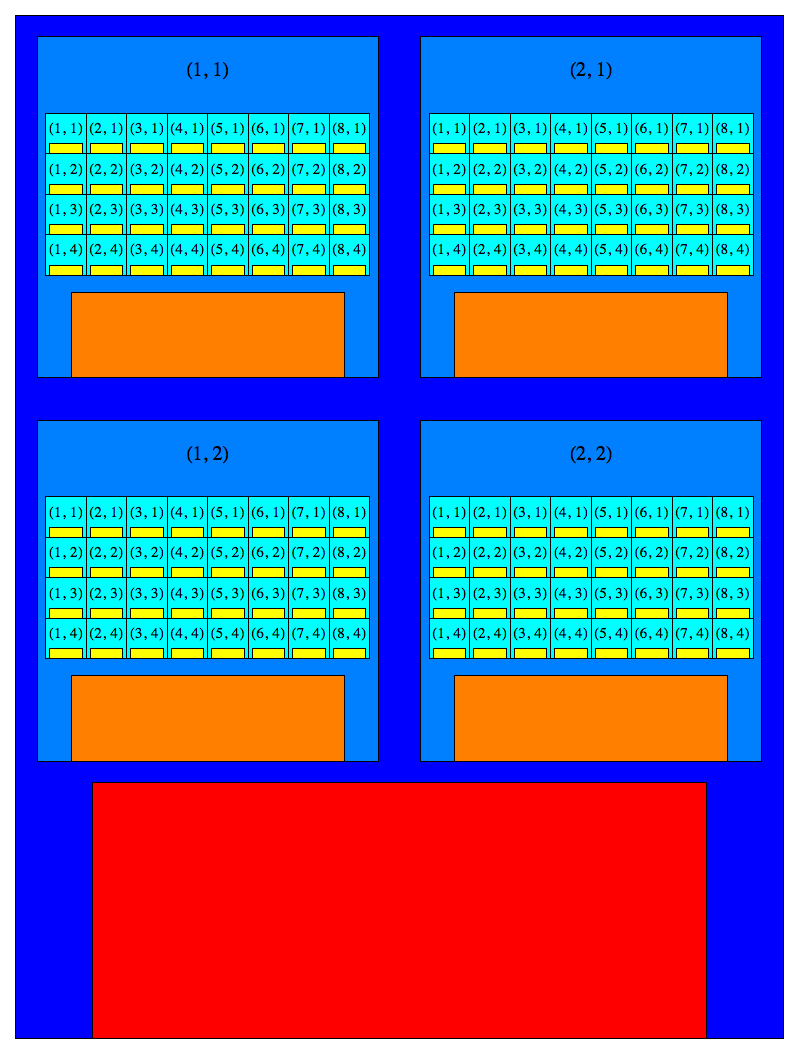
\includegraphics[width=0.83\textwidth]{Figures/gpu_arc.png}
\caption[Architecture of a GPU]
{Architecture of a GPU. Organization of threads and blocks in the grid, and the location of different memory types within them. The grid is coloured dark blue, blocks are coloured light blue, and threads are coloured cyan. The global memory is coloured red, shared memory is coloured orange, and register memory is coloured yellow. The numbers in parenthesis indicate the block or thread's $blockIdx$ or $threadIdx$ variables. In this particular case, $blockDim=(8,4)$ and $gridDim=(2,2)$. A thread is able to access memory that is inside its registers, but not the registers of other threads, and memory that is inside the shared memory of its block, but not the shared memory of other blocks. All threads can access all of the global memory.}
\label{fig:gpuarc}
\end{figure}

\subsection{Occupancy and Performance}
\label{sec:gpuocc}
Having described the various resources, we can talk about how they can be used most effectively. The occupancy of a kernel is the number of warps that are actually able to run on a SM divided by the maximum possible warps an SM can run. Occupancy is important, as it determines the maximum number of blocks, and thus threads that are able to run simultaneously. The occupancy of a kernel is determined by three factors: the block size, the amount of shared memory per block, and the number of registers used per thread. While block size and shared memory are explicitly set by the programmer, it is next to impossible to guess how registers will be used before compile time. Thankfully, there are compiler flags that will display this information.

Armed with the resources our kernel will need, we can now determine its occupancy. The ``CUDA Occupancy Calculator" is an Excel spreadsheet provided by NVIDIA and is an indispensable tool. We can input the needed resources and the hardware generation of our card and then receive the occupancy of the current resource configuration, where the bottleneck of the current configuration is, as well as information on how the occupancy will change upon tweaking the configuration. In some sense, the best block size is determined by how the other resources are used. Therefore, in order to maximize the occupancy, we must first make sure that we are correctly using the memory provided.

Registers are the fastest memory available, but they are also the easiest to overuse. Therefore, they are best suited for small variables that need to be referenced frequently, such as accumulators. Shared memory is best used for storing large sections of non-contiguous data stored in the global memory. Finally, data that is able to be stored such that it can be accessed effectively, or is infrequently used, might best be left in the global memory.

As with everything, these rules are only guidelines. The best resource configuration will be individual not only to every kernel, but also to the GPU it is to be run on. The best way to maximize the efficiency of a calculation is to make minor alterations to where data is stored and play around with the code. Finally, it might not always be the best idea to maximize the occupancy of a kernel. If the bottleneck is not the actual calculation, but how fast the data can be read, then it might be advantageous to fill up the registers and shared memory as much as possible and have a very low occupation.

\subsection{Matrix Multiplication Example}
To complete the introduction to CUDA programming, we will go over a real example of CUDA Fortran code. For our example, we will examine code that performs matrix multiplication on matrices of arbitrary dimensions. This makes use of all the concepts we've covered so far, so it will be a good exercise to examine. The code is given below.
\lstinputlisting[caption={Matrix multiplication kernel}]{code_snippets/mat_mul.cuf}

Lines 1 - 43 define a module which contains a matrix multiplication kernel. The kernel takes the matrices \texttt{inputA} and \texttt{inputB}, multiplies them, and stores the result in \texttt{output}. The kernel has the \texttt{{\color{myblue}{attributes}}(global)} attribute, which means that it can be called from either device or host code. \texttt{rowA}, \texttt{colA}, \texttt{rowB}, and \texttt{colB} are the rows and columns of \texttt{inputA} and \texttt{inputB}. Because they are small and don't change over the course of the calculation, they get stored in a special memory type called constant memory. This is a small cache of read only memory that is 64KB in size and allows for constant values to be read very quickly. There are two shared variables, \texttt{s\_tileA} and \texttt{s\_tileB}. Each of these are square matrices with dimensions of \texttt{block\_dim} and these will be used to store sections or ``tiles" of \texttt{inputA} and \texttt{inputB} respectively. We want each thread to do all the calculations needed to compute a simple element of \texttt{output}. Line 13 and 14 use the \texttt{threadIdx}, \texttt{blockDim}, and \texttt{blockIdx} variables so that each thread gets a unique combination of \texttt{x} and \texttt{y} values. \texttt{x} corresponds to a row of the \texttt{output} matrix and \texttt{y} corresponds to a column, so each thread is then uniquely mapped to an element of \texttt{output}. We will see in the host code how these index values are determined, but for now it is sufficient to know that there will be at least as many threads as elements of \texttt{output}.

Lines 17 - 37 are where the actual calculation takes place. For each iteration of the loop, a different tile of \texttt{inputA} and \texttt{inputB} is fetched from the global memory and stored into the shared memory. The reason for using this tiling approach can be seen when we consider how the threads must read \texttt{inputB}. If we did not use shared memory, the loop would just be \texttt{total {\color{myyellow}{=}} total {\color{myyellow}{+}} inputA(x, i) {\color{myyellow}{*}} inputB(i, y)}. In this case, access to \texttt{inputA} is coalesced, but access to \texttt{inputB} is not. Therefore, the kernel will be stunted due this unoptimized memory usage. Instead, we load tiles in a coalesced manner into the shared memory, synchronize the threads, and then read through the shared memory in an uncoalesced fashion which carries no penalty. At the end of each loop, the tiles are moved in the \texttt{y} direction for \texttt{inputA} and in the \texttt{x} direction for \texttt{inputB}, and the process repeats. Notice how it is possible that a tile might fall on the boundary of an \texttt{input} matrix. This is why there are checks to make sure the coordinates of the tile don't exceed the boundaries of a matrix so we don't start reading garbage.

In the host code on lines 45 - 102, we have two sets of variables, those for the host and those for the device. Notice how device variables have the \texttt{{\color{mygreen}{device}}} attribute. For clarity, they are given the same name as their host variables but with a \texttt{d\_} prefix. We now assign constant variables from line 5 to arbitrary values. Next we set up the random number generator, allocate the host matrices memory, and randomly initialize the input matrices. Then the device variables are allocated memory and the host data is then uploaded to the GPU. The block and grid dimensions are set up on lines 87 and 88. \texttt{blockDim} and \texttt{gridDim} are variables of \texttt{{\color{mygreen}{type}}(dim3)} which is a tuple that is defined in the \texttt{cudafor} module. The block has two dimensions containing \texttt{block\_dim}$^{2}$ threads. The grid also has two dimensions, and as we need one thread per element of \texttt{output} we perform a calculation which returns the minimum number of blocks that will cover it. Finally, we launch the kernel on line 90 using the \texttt{\color{myyellow}{<<< >>>}} operators to provide the grid and block dimensions, download the result from the GPU, and deallocate the memory.

\section{Program flow in cudaDFRATOM}
In this section, the control flow of a typical calculation is given.

\textit{Step 1}. The input file is read by the \textit{\textbf{intin}} subroutine. If needed, the basis set and open-shell configurations are calculated by \textit{\textbf{formbs}} and \textit{\textbf{find\_bin\_configurations}} respectively. The options set in the input file are rewritten to stdout.

\textit{Step 2}. The calculation of small arrays and other constants is performed by \textit{\textbf{calc\_parameters}} and \textit{\textbf{bsnorm}}. \textit{\textbf{calc\_parameters}} calls \textit{\textbf{bcoef}} and \textit{\textbf{setvc}}.

\textit{Step 3}. The mapping of threads to the unrolled one and two-electron integral matrixes are calculated by \textit{\textbf{lmpqrsa}} on the GPU. All other data from step 1 and 2 is then uploaded to the GPU.

\textit{Step 4}. The one and two electron integrals are calculated on the GPU by \textit{\textbf{eint1gpu}} and \textit{\textbf{eint2gpu}} respectively.

\textit{Step 5}. The initial guess of the density matrix is calculated by \textit{\textbf{guess}} on the GPU. This is done by the diagonalization of the one-electron Hamiltonian matrix.

\textit{Step 6}. \textit{\textbf{scfiter}} then performs the SCF iterations until convergence of the density matrix has been reached, or the maximum number of iterations has been reached. SCF is performed with cuSOLVER functions, as well as a few custom helper functions. The converged eigenvectors, values, and energies are downloaded from the GPU and then written to stdout.

\textit{Step 7} (optional). If jobtyp=`bsopt', then an optional basis set optimization is carried out. This starts by assigning pointers to variables on the CPU and GPU through \textit{\textbf{hookup\_cpu}} and \textit{\textbf{hookup\_gpu}}. Then, the four well-tempered basis set (WTBS) parameters are optimized by \textit{\textbf{newuoa}}. \textit{\textbf{newuoa}} calls \textit{\textbf{calc\_energy}} which essentially reconstructs the basis set from new parameters from \textit{\textbf{newuoa}}, then repeats steps 2 - 6 and feeds the energy back into \textit{\textbf{newuoa}}. This repeats until optimal WTBS parameters have been found.

\section{Alterations of DFRATOM for CUDA}
While almost all of the code from the original DFRATOM\cite{MATSUOKA2001218} was modified in some way, the most extreme changes were the integral evaluation and the formation of the P and Q matrixes. Therefore, we will discuss these changes in detail in this section.

\subsection{Two-electron Integrals}
The original DFRATOM calculates the two electron integrals with a long series of nested \textbf{for} loops. Working from the outside in, the indices of the loops are $L$, $P$, $Q$, $M$, $R$, and $S$ where $L$ and $M$ are spinor symmetries, $P$ and $Q$ are basis functions of symmetry $L$, and $R$ and $S$ are basis functions of symmetry $M$. The pseudocode for these is shown in Algorithm \ref{origcode} where $nsym$ is the total number of symmetries, and $nbs(i)$ is the number of basis functions for symmetry species $i$. Thus, each set of J and K integrals is uniquely defined by its $L$, $M$, $P$, $Q$, $R$, and $S$ values. In order to have an effective CUDA implementation of this algorithm, we need to find a way to map these six numbers to CUDA threads. The simplest approach would be to map the values of $L$, $P$, and $Q$ onto the $threadIdx.x$, $threadIdx.y$, and $threadIdx.z$ variables for each thread, launch the needed number of blocks, and then have each thread loop over the remaining indices. The pseudocode for this can be seen in Algorithm \ref{easycode}. A similar method is employed by many other programs, and for larger systems it works perfectly well. But because this program is for only single atoms, problems begin to appear.

\begin{algorithm}
\caption{The original }
\label{origcode}
\begin{algorithmic}
\FOR{$L = 1$ to $nsym$}
	\FOR{$P = 1$ to $nbs(L)$}
		\FOR{$Q = 1$ to $P$}
			\FOR{$M = 1$ to $L$}
				\IF{$L = M$}
					\STATE{$maxr$ = $P$}
				\ELSE
					\STATE{$maxr$ = $nbs(M)$}
				\ENDIF
				\FOR{$R = 1$ to $maxr$}
					\IF{$(L = M)$ \AND $(P = R)$}
						\STATE{$maxs$ = $Q$}
					\ELSE
						\STATE{$maxs$ = $R$}
					\ENDIF
					\FOR{$S = 1$ to $maxs$}
						\STATE{compute the J and K integrals of $L$, $M$, $P$, $Q$, $R$, and $S$}
					\ENDFOR
				\ENDFOR
			\ENDFOR
		\ENDFOR
	\ENDFOR
\ENDFOR
\end{algorithmic}
\end{algorithm}

\begin{algorithm}
\caption{Easy code}
\label{easycode}
\begin{algorithmic}

\STATE{$L = threadIdx.x + (blockIdx.x - 1) * blockDim.x$}
\STATE{$P = threadIdx.y + (blockIdx.y - 1) * blockDim.y$}
\STATE{$Q = threadIdx.z + (blockIdx.z - 1) * blockDim.z$}
\STATE{}
\IF{$(L \leq nsym)$ \AND $(P \leq nbs(L))$ \AND $(Q \leq P)$}
			\FOR{$M = 1$ to $L$}
				\IF{$L = M$}
					\STATE{$maxr$ = $P$}
				\ELSE
					\STATE{$maxr$ = $nbs(M)$}
				\ENDIF
				\FOR{$R = 1$ to $maxr$}
					\IF{$(L = M)$ \AND $(P = R)$}
						\STATE{$maxs$ = $Q$}
					\ELSE
						\STATE{$maxs$ = $R$}
					\ENDIF
					\FOR{$S = 1$ to $maxs$}
						\STATE{compute the J and K integrals of $L$, $M$, $P$, $Q$, $R$, and $S$}
					\ENDFOR
				\ENDFOR
			\ENDFOR
\ENDIF
\end{algorithmic}
\end{algorithm}

The first problem arises due to warp divergence: as the maximum values of $M$, $R$, and $S$ depend on $L$, $P$, and $Q$, different threads will have a different number of loops to complete than others. Because a streaming multiprocessor (SM) must finish the block it is currently working on before it can grab another, there is the possibility that most of the threads in a block are idling while waiting for others in the same block to finish. The second problem with this method is that there will always be several blocks which have threads that remain idle throughout the block's runtime, no matter what. This can be seen more clearly in Figure \ref{fig:naivelayout}. The third problem with this is that with the maximum values for $L$, $P$, and $Q$ available for a single atom, there might not even be enough combinations to completely fill the GPU. While all of these issues begin to disappear once the number of integrals to evaluate becomes large enough, we are still very much in the range where they are in play. Therefore a smarter algorithm had to be used.

\begin{figure}[h!]
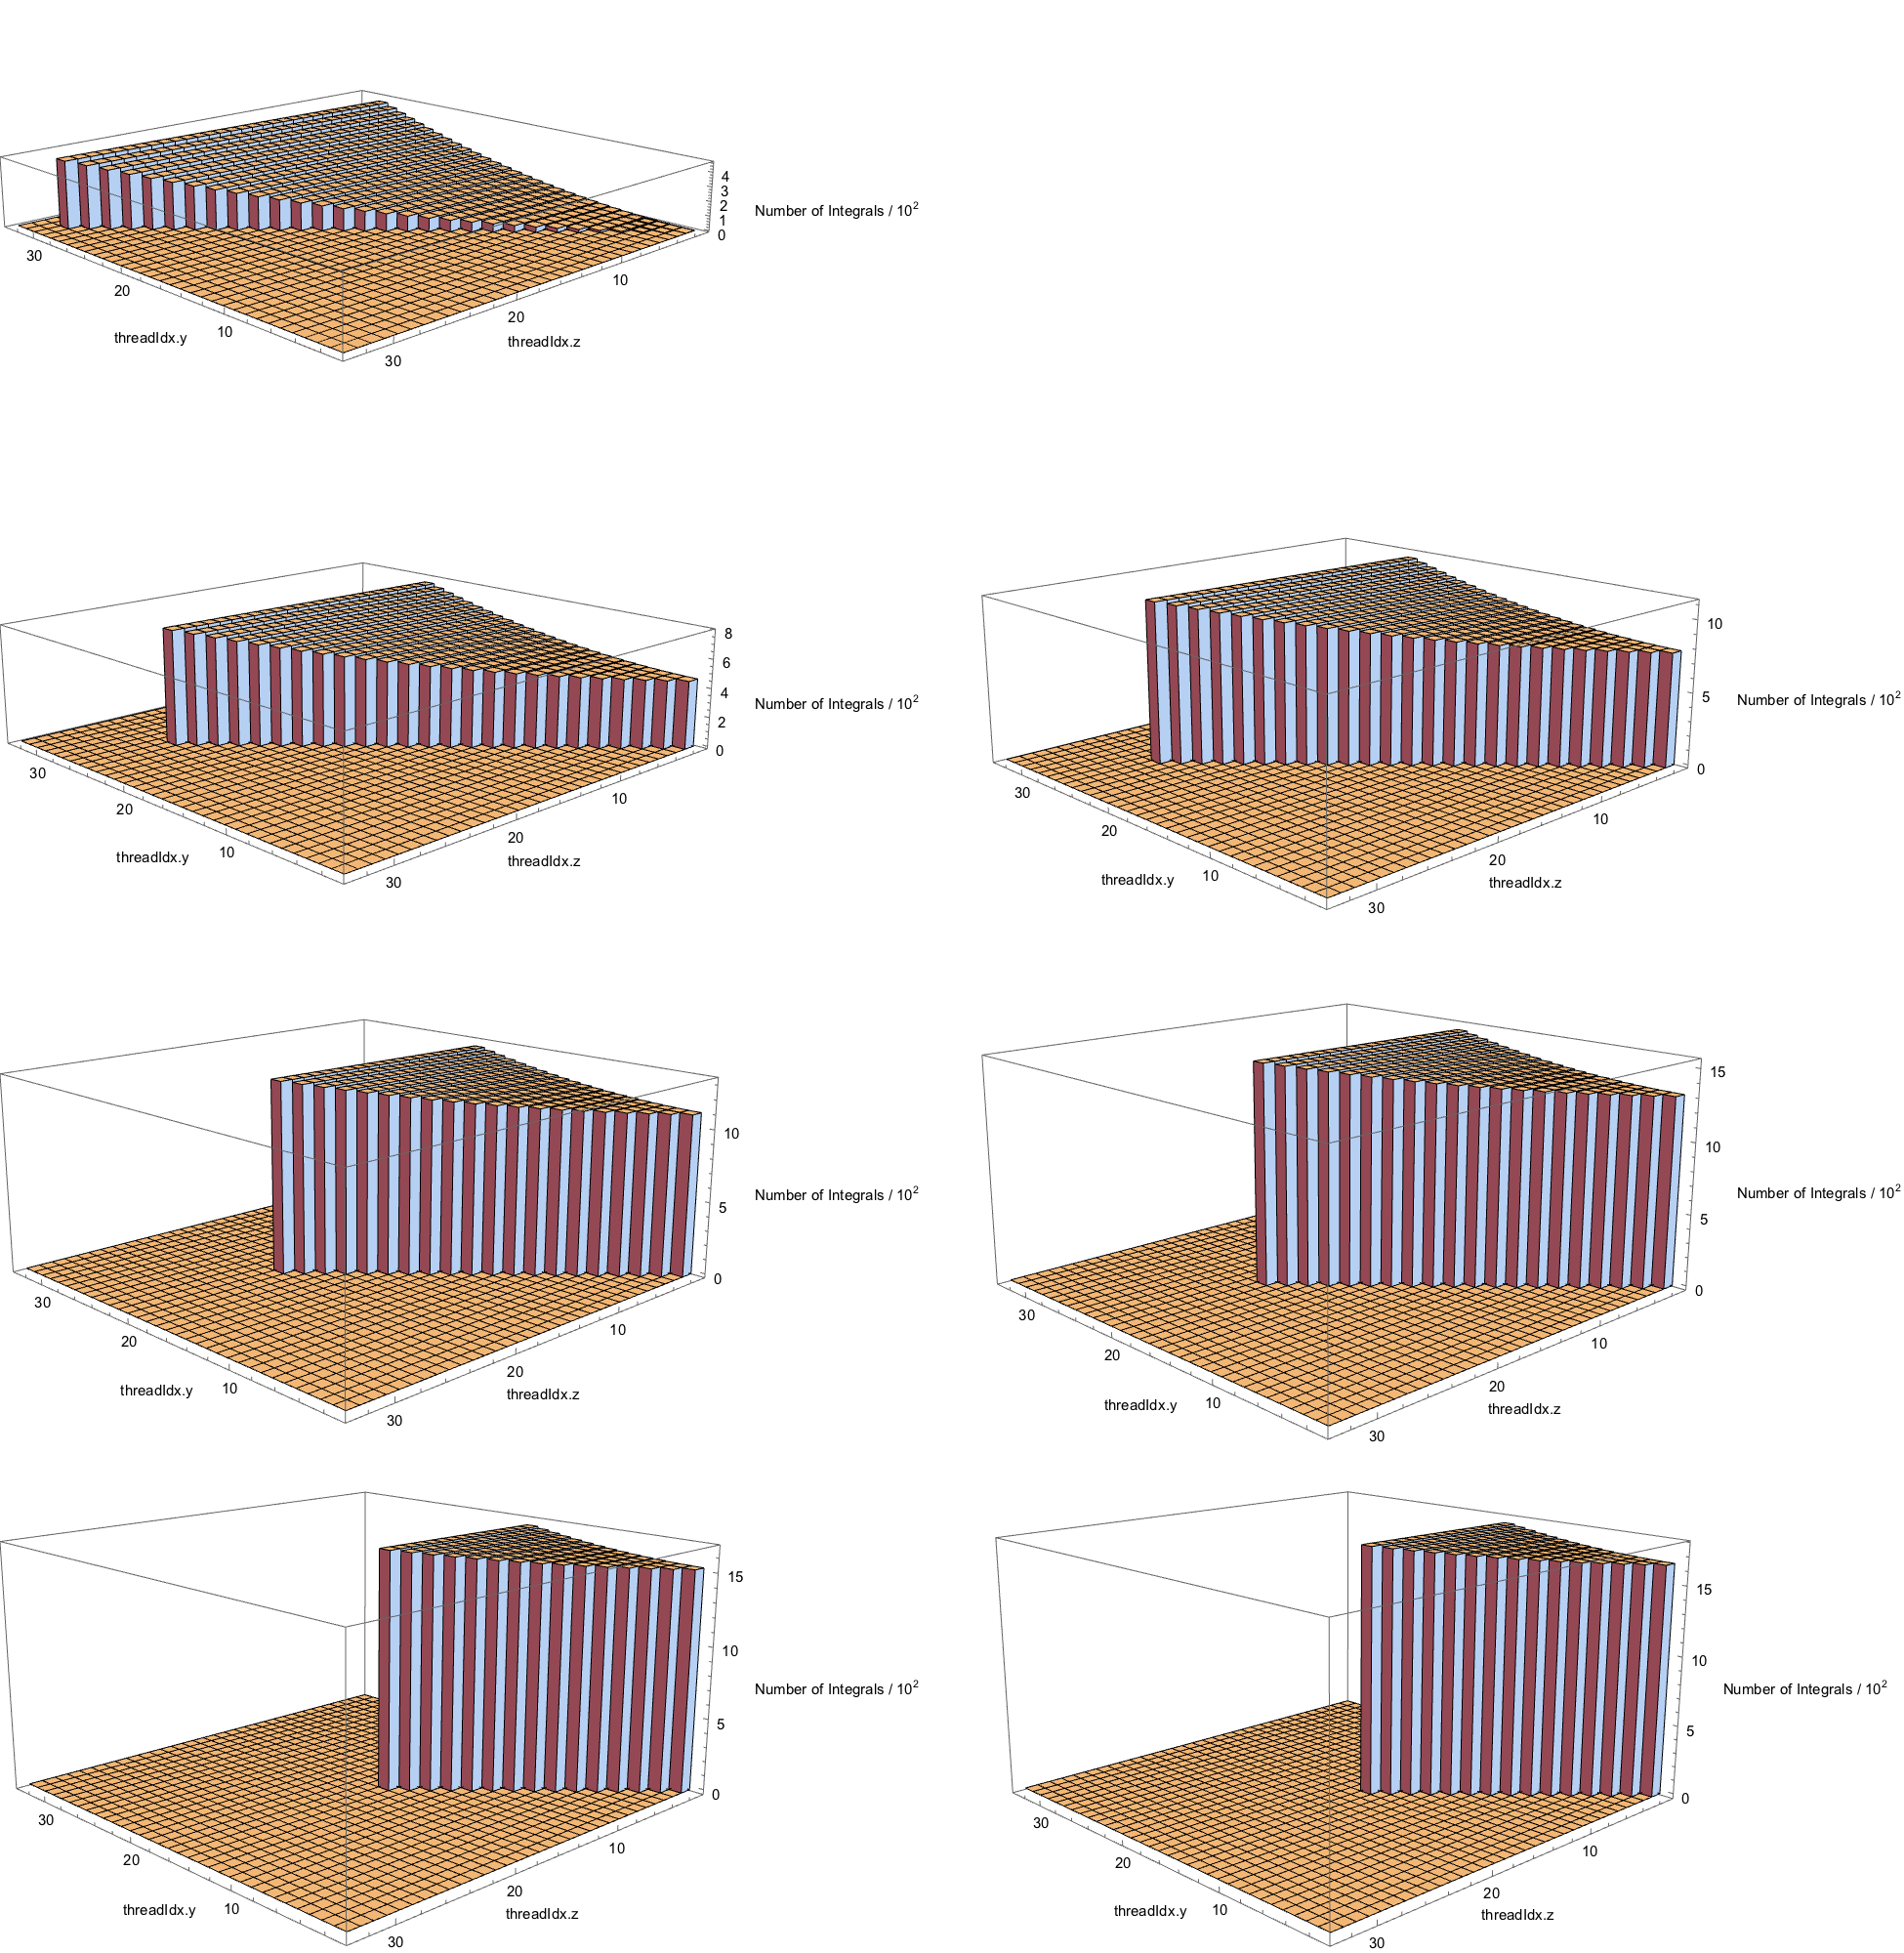
\includegraphics[width=1\textwidth]{Figures/30_25_20_15_naive_layout.png}
\caption[Two-electron integral layout: naive implementation.]
{Two-electron integral layout: naive implementation. Mapping of integrals to threads using Algorithm \ref{easycode}. The basis set used had $nsym = 7$ with $nbs(i)=(30,25,25,20,20,15,15)$. The $blockDim = (1, 32, 32)$ and $gridDim = (7, 1, 1)$. Each histogram is one block of threads, where the horizontal axes are the $threadIdx.y$ and $threadIdx.z$ variables, and the vertical axis is the number of Two-Electron Integrals it must compute. Notice that in all blocks there are threads that calculate no integrals and therefore are idle throughout the lifetime of the block. Also note that the number of integrals each thread must calculate grows both from block to block, and from thread to thread within a block. Both of these factors make this algorithm an undesirable choice.}
\label{fig:naivelayout}
\end{figure}

The second problem can be solved by restricting the dimensionality of the solution instead of the using the three dimensional one of Algorithm \ref{easycode}. We might consider using a two dimensional solution, but then we still will have blocks with idle threads which can be seen in Figure \ref{fig:genmatblock}. By restricting ourselves to only using $threadIdx.x$, we ensure that only the last block to run will have the possibility of having threads remaining idle throughout the block's runtime as shown in Figure \ref{fig:genvecblock}. 

The first and third problems can be solved by having each thread calculate one and only one set of J and K integrals. If we start with a valid combination of $L$, $M$, $P$, $Q$, $R$, and $S$ values, we can very easily figure out which thread will calculate that set of integrals by using the following equations:

\begin{figure}[h!]
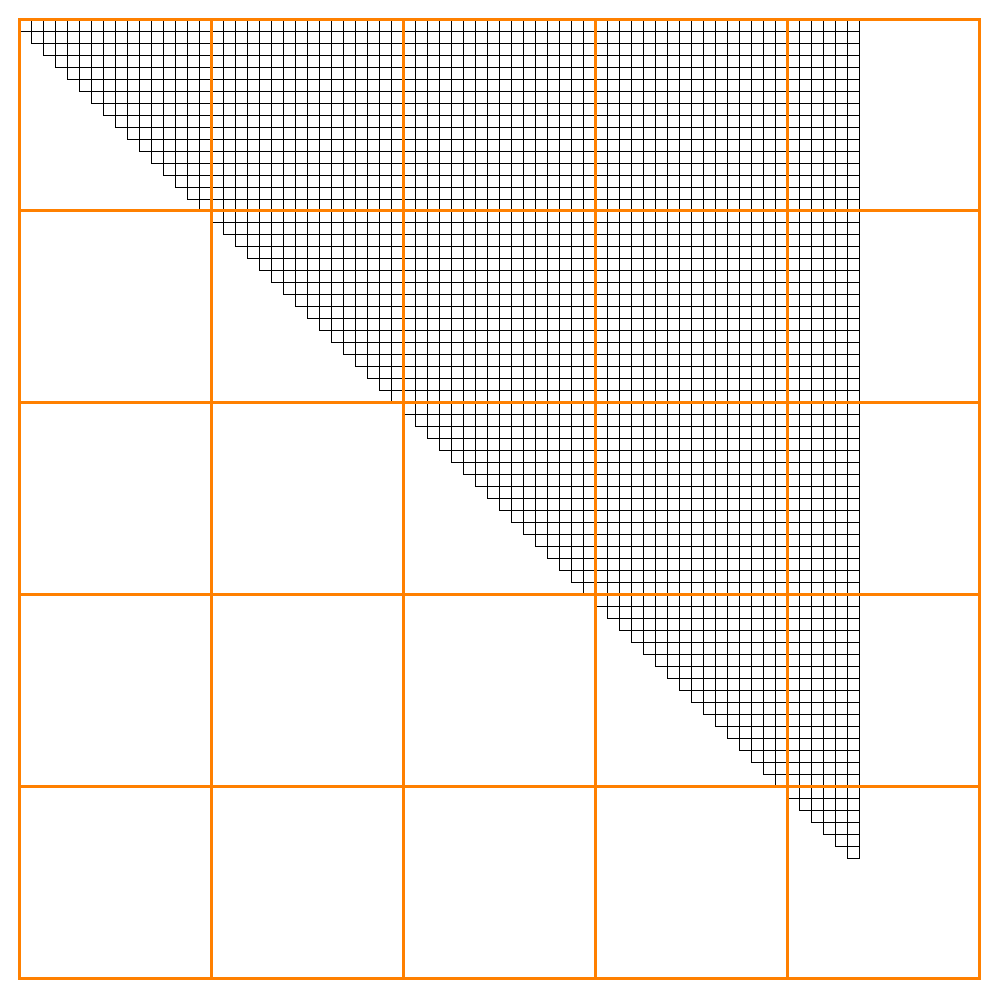
\includegraphics[width=1\textwidth]{Figures/gen_mat_block_layout.png}
\caption[Two-electron integral layout: 2D blocks and grid]
{Two-electron integral layout: 2D blocks and grid. Orange lines indicate the border of blocks. Notice that many blocks have idle threads.}
\label{fig:genmatblock}
\end{figure}

\begin{figure}[h!]

\includegraphics[width=1\textwidth]{Figures/gen_vec_block_layout.png}
\caption[Two-electron integral layout: 1D blocks and grid]
{Two-electron integral layout: 1D blocks and grid. Orange lines indicate the border of blocks. Notice that only the last block contains idle threads.}
\label{fig:genvecblock}
\end{figure}

\begin{equation}
\label{nprime}
n'(j) = \frac{j^{2}+j}{2}
\end{equation}

\begin{equation}
\label{ylpq}
y = n'(nbs(L - 1)) + n'(P - 1) + Q
\end{equation}

\begin{equation}
\label{xmrs}
x = n'(nbs(M - 1)) + n'(R - 1) + S
\end{equation}

\begin{equation}
\label{numtothread}
i = n'(x) + y
\end{equation}

\begin{equation}
\label{imax}
i_{max} = n'(\sum^{nsym}_{j = 1}n'(nbs(j)))
\end{equation}

where $nbs(0) = 0$ and $i=threadIdx.x + (blockIdx.x - 1) * blockDim.x$. Starting with a value of $i$ and working our way back is a much more challenging task. It becomes easier if we reframe it in the following way.

\clearpage

Consider Figures \ref{fig:eint2mat} and \ref{fig:eint2vec}. Figure \ref{fig:eint2mat} shows the top half of the symmetric two-electron integral matrix for a problem with $nsym = 2$ and 3 basis function for symmetry one, and 2 for symmetry two. Figure \ref{fig:eint2vec} shows the same but mapped onto a vector representation. In each element of both figures there is a set of seven numbers. The top two are $L$ and $M$, then $P$ and $Q$, then $R$ and $S$, and the last number is the value of $i$ for the thread calculating that integral. With this, it can be seen from the matrix representation that each element in the same row have the same $M$, $R$, and $S$ values and the elements in the same column have the same $L$, $P$, and $Q$ values. Therefore, finding out which column the element belongs to gives us the value for $y$, and finding the row give us the value of $x$. This can be done with the binary search algorithm shown in Algorithm \ref{bsxy}.

\begin{figure}[h!]
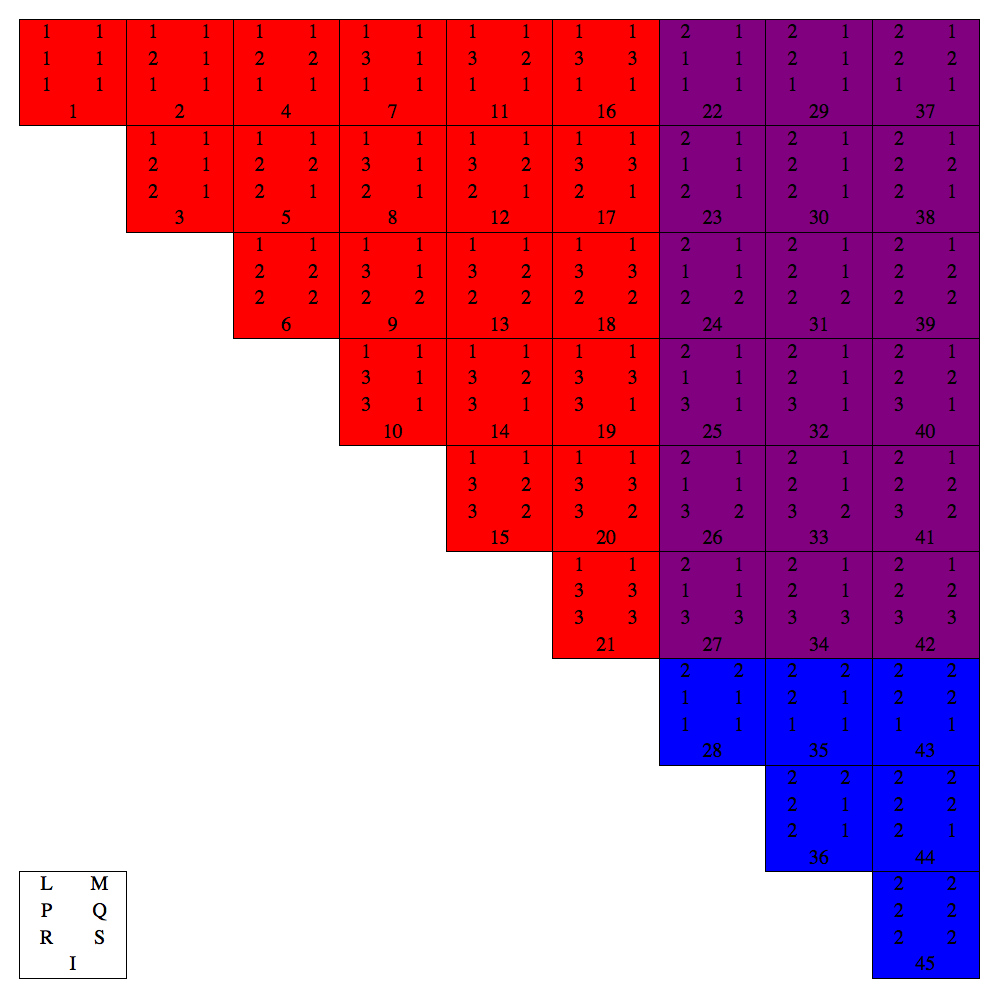
\includegraphics[width=1\textwidth]{Figures/eint2_mat.png}
\caption[Two-electron integral matrix as a matrix]
{Two-electron integral matrix as a matrix: The top triangle of the two-electron symmetric matrix in a matrix representation. In this instance, the total number of symmetries is 2, with 3 basis functions for the first symmetry and 2 basis functions for the second. The key for translating the numbers in each box into the $L$, $M$, $P$, $Q$, $R$, and $S$ values is given in the bottom left. Notice how all rows have the same $M$, $R$, and $S$ values, while all columns have the same $L$, $P$, and $Q$ values. For clarity, the boxes have been coloured, based on the spinor symmetries that they contain.}
\label{fig:eint2mat}
\end{figure}

\begin{figure}[h!]
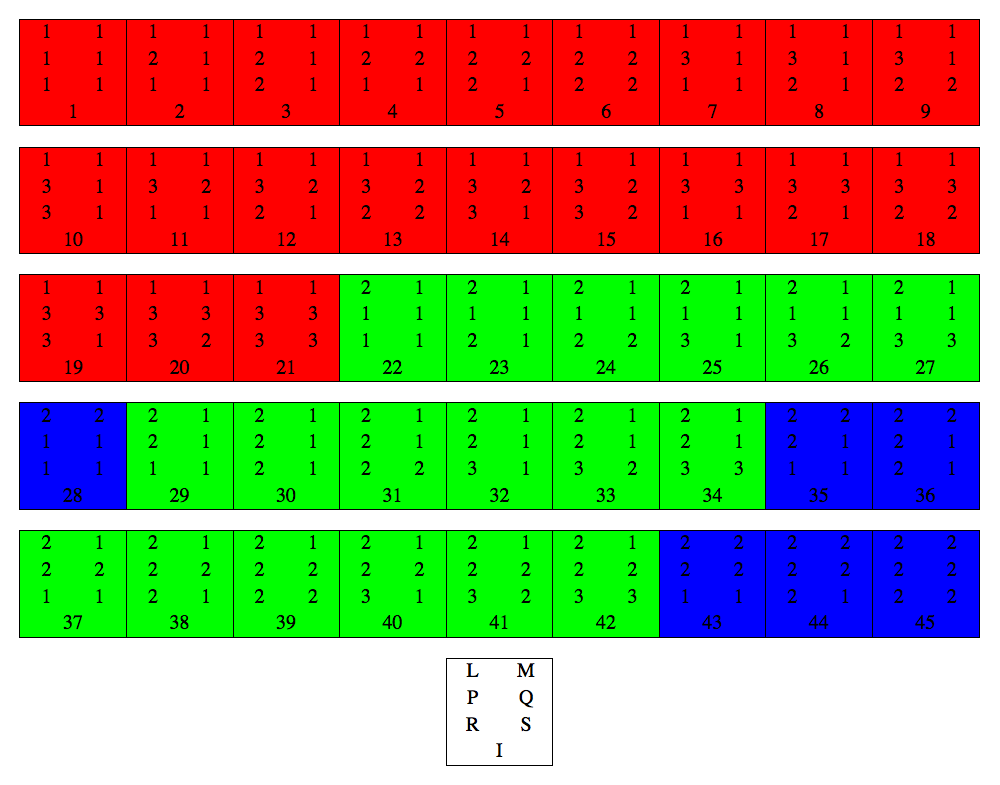
\includegraphics[width=1\textwidth]{Figures/eint2_vec.png}
\caption[Two-electron integral matrix as a vector]
{Two-electron integral matrix as a vector: The top triangle of the two-electron symmetric matrix in a vector representation. In this instance, the total number of symmetries is 2, with 3 basis functions for the first symmetry and 2 basis functions for the second. The key for translating the numbers in each box into the $L$, $M$, $P$, $Q$, $R$, and $S$ values is given in the bottom center. Notice how the $L$, $M$, $P$, $Q$, $R$, and $S$ values are much harder to predict than from the matrix representation. For clarity, the boxes have been coloured based on the spinor symmetries that they contain. Gaps between rows are used to reinforce that the elements are not connected like a matrix.}
\label{fig:eint2vec}
\end{figure}


\begin{algorithm}[h!]
\caption{Binary search for $x$ and $y$}
\label{bsxy}
\begin{algorithmic}

\IF{$theadIdx.x \leq nsym$}
	\STATE{$s\_nsym = nsym$}
	\STATE{$s\_nbs(threadIdx.x) = nbs(threadIdx.x)$}
	\STATE{$s\_nprime(threadIdx.x) = n'(s\_nbs(threadIdx.x))$}
\ENDIF

\STATE{call \textbf{syncthreads}}

\STATE{$i =  threadIdx.x + (blockIdx.x - 1) * blockDim.x$}
\IF{$i \leq i_{max}$}
	\STATE{$low = 1$}
	\STATE{$high = \textbf{sum}(s\_nprime(1:s\_nsym))$}
	\WHILE{$low \leq high$}
		\STATE{$mid = \frac{(low + high)}{2}$}
		\STATE{$lownum = \frac{(mid - 1)(mid - 2)}{2} + mid$}
		\STATE{$highnum = lownum - 1 + mid$}
		\IF{$(i \leq highnum)$ \AND $(i \geq lownum)$}
			\STATE{$y = mid$}
			\STATE{\textbf{exit}}
		\ELSIF{$i > highnum$}
			\STATE{l$ow = mid + 1$}
		\ELSIF{$i < lownum$}
			\STATE{$high = mid - 1$}
		\ENDIF
	\ENDWHILE
	\STATE{$x = i - lownum + 1$}
\ENDIF

\end{algorithmic}
\end{algorithm}

In this algorithm, variables with the $s\_$ prefix refer to those in the shared memory, and $lownum$ and $highnum$ refer to the minimum and values that $i$ could have for the current guess ($mid$) of $y$. From here, $L$ can be found with Algorithm \ref{bsL}, and $P$ and $Q$ can be found with Algorithm \ref{bsPQ}. The same set of algorithms can then be used to get $M$, $R$, and $S$ by substituting the relevant variables. If there is sufficient global memory available, these values can be stored and referred to later as needed. Otherwise, they could be calculated on the fly as needed. Because binary search scales as $\mathcal{O}(n\log{}n)$, this should ensure that this remains a fast method of mapping threads to integrals for large problems as well. With some alterations, this method could also apply to molecular symmetries and not only to a single atom. For instance in the C$_{1}$ symmetry, all possible combinations of four basis functions must be used (ignoring those that appear on the bottom triangle of the two electron integral matrix of course). We could simply remove the search for $L$ and $M$, have the initial value of $high$ in Algorithm \ref{bsPQ} be the total number of basis functions, and remove the \textbf{sum}$(s\_nprime(1:L-1)$ term from $lownum$.

\begin{algorithm}
\caption{Binary search for $L$}
\label{bsL}
\begin{algorithmic}

\STATE{$i =  threadIdx.x + (blockIdx.x - 1) * blockDim.x$}
\IF{$i \leq i_{max}$}
	\STATE{$low = 1$}
	\STATE{$high = s\_nsym$}
	\WHILE{$low \leq high$}
		\STATE{$mid = \frac{(low + high)}{2}$}
		\STATE{$lownum = 1 + \textbf{sum}(s\_nprime(1:mid-1)$}
		\STATE{$highnum = lownum - 1 + s\_nprime(mid)$}
		\IF{$(i \leq highnum)$ \AND $(i \geq lownum)$}
			\STATE{$L = mid$}
			\STATE{\textbf{exit}}
		\ELSIF{$y > highnum$}
			\STATE{$low = mid + 1$}
		\ELSIF{$y < lownum$}
			\STATE{$high = mid - 1$}
		\ENDIF
	\ENDWHILE
\ENDIF

\end{algorithmic}
\end{algorithm}

\begin{algorithm}
\caption{Binary search for $P$ and $Q$}
\label{bsPQ}
\begin{algorithmic}

\STATE{$i =  threadIdx.x + (blockIdx.x - 1) * blockDim.x$}
\IF{$i \leq i_{max}$}
	\STATE{$low = 1$}
	\STATE{$high = s\_nbs(L)$}
	\WHILE{$low \leq high$}
		\STATE{$mid = \frac{(low + high)}{2}$}
		\STATE{$lownum =  \frac{(mid - 1)(mid - 2)}{2} + mid + \textbf{sum}(s\_nprime(1:L-1))$}
		\STATE{$highnum = lownum + mid - 1$}
		\IF{$(i \leq highnum)$ \AND $(i \geq lownum)$}
			\STATE{$P = mid$}
			\STATE{\textbf{exit}}
		\ELSIF{$y > highnum$}
			\STATE{$low = mid + 1$}
		\ELSIF{$y < lownum$}
			\STATE{$high = mid - 1$}
		\ENDIF
	\ENDWHILE
	\STATE{$Q = y - lownum + 1$}
\ENDIF

\end{algorithmic}
\end{algorithm}

From here, the new code for evaluating the integrals remains largely the same as the original, except for some minor changes to allow for more efficient global or shared memory access. We also use a process referred to as ``grid-stride looping" where all these binary search algorithms have their \textbf{if} $i \le i_{max}$ \textbf{then} removed, and then are placed within the following loop: \textbf{for} $i = threadIdx.x + (blockIdx.x - 1) * blockDim.x$ to $i_{max}$, $i \mathrel{+}= blockDim.x * gridDim.x$ \textbf{do}. If we know the occupancy of the algorithm on the GPU beforehand, we can launch exactly the number of blocks that will fill the GPU. This reduces the overhead of block swapping and lets us further eke out some performance.

\subsection{Density Matrix Formation}
The term in parenthesis in Equation \ref{FOCKM} corresponds to the non-relativistic density matrix. But as we are interested in relativistic calculations, it will need to be altered. Firstly, because a relativistic wavefunction has both large and small components, so too does its density matrix. Therefore, it will have two dimensions that span from 1 to $2K$ where dimensions 1 to $K$ are the large components and the rest are for small components. Secondly, the factor of 2 is replaced by the number of electrons that can occupy spinors of symmetry $\mu$. The density matrix's matrix and vector representations are shown in Figures \ref{fig:dtmxmat} and \ref{fig:dtmxvec} respectively. The mathematical form of the density matrix is given in Equation \ref{RDCMX}\cite{MATSUOKA2001218}

\begin{equation}
\label{RDCMX}
\textbf{D$_{\textbf{C}r,s}$} =N_{\mu}\sum^{occ}_{a=1}\textbf{C}_{r,a}\textbf{C}^{*}_{s,a}
\end{equation}

\begin{figure}
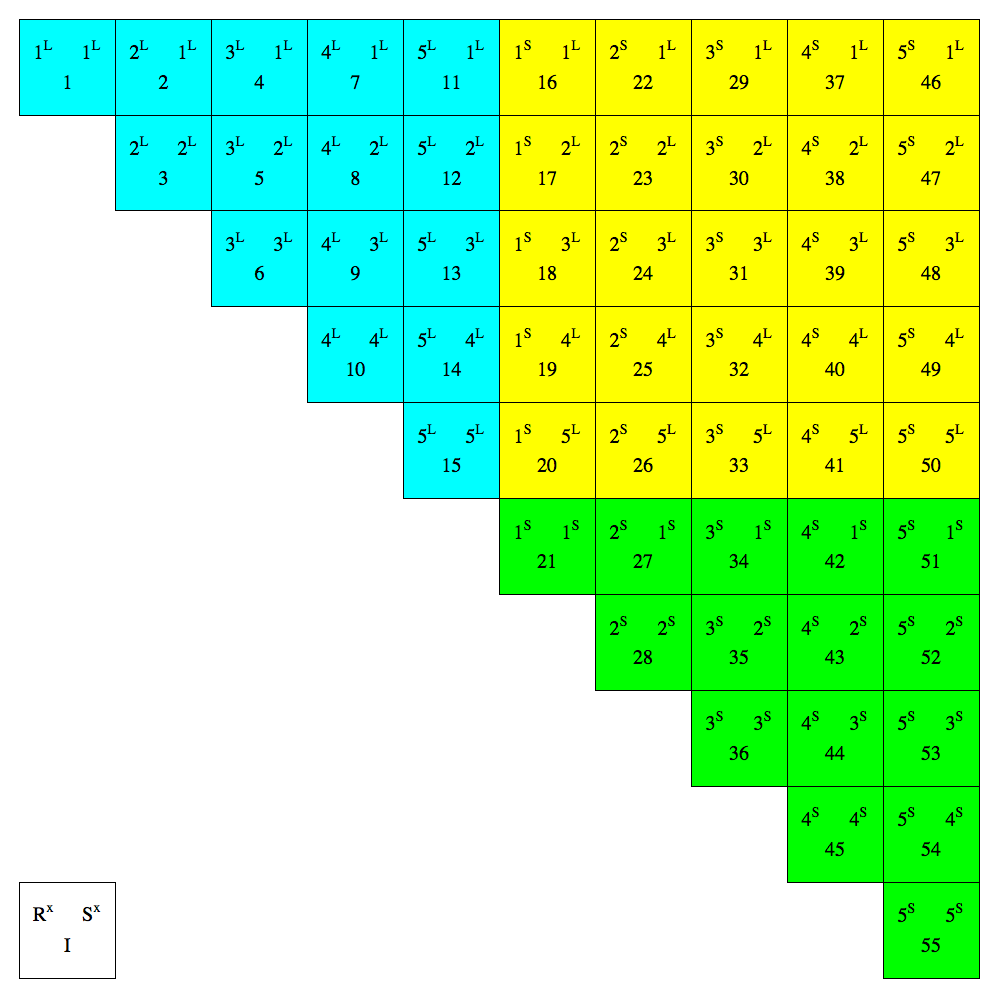
\includegraphics[width=1\textwidth]{Figures/dtmx_mat.png}
\caption[Density matrix as a matrix]
{Density matrix as a matrix. The top triangle of the symmetric density matrix in a matrix representation. The key for translating the numbers in each box into the $R$ and $S$ values is given in the bottom right. All active symmetries would have a similar, separate matrix. For clarity, the elements have been colorized based on the combination of large and small components they contain.}
\label{fig:dtmxmat}
\end{figure}

\begin{figure}
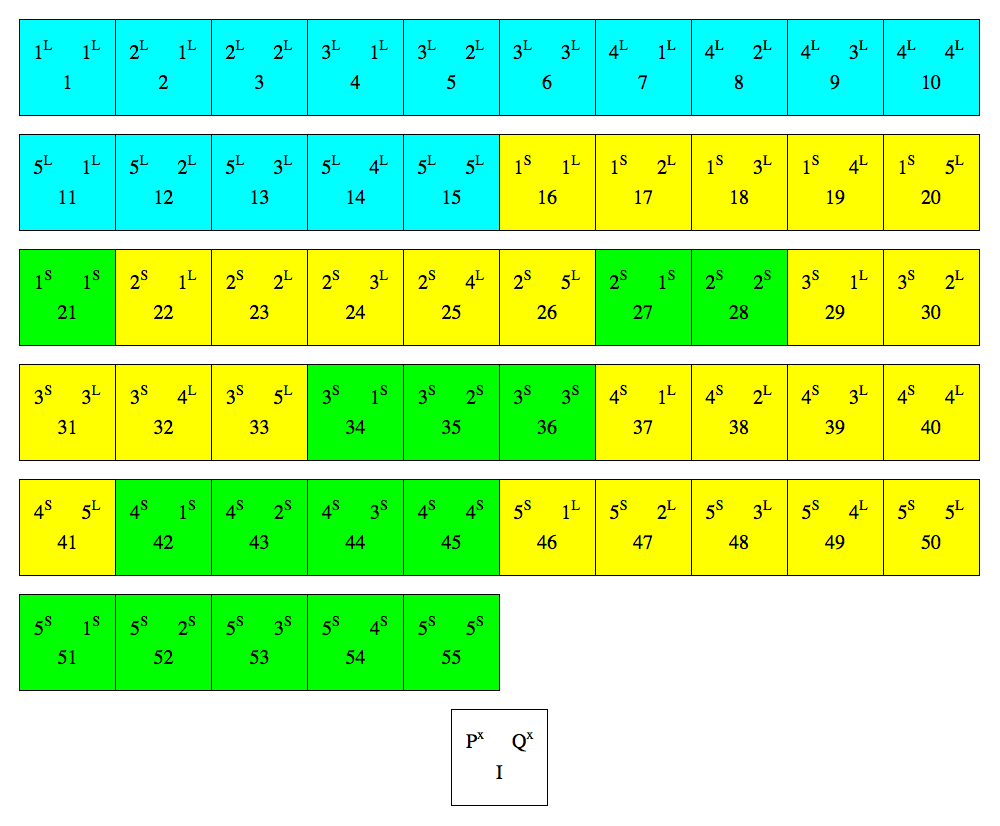
\includegraphics[width=1\textwidth]{Figures/dtmx_vec.png}
\caption[Density matrix as a vector]
{Density matrix as a vector. The top triangle of the symmetric density matrix in a vector representation. The key for translating the numbers in each box into the $R$ and $S$ values is given in the bottom left. All active symmetries would have a similar, separate vector that continue one after the other. For clarity, the elements have been colorized based on the combination of large and small components they contain.}
\label{fig:dtmxvec}
\end{figure}


where $N_{i}$ is the number of electrons that occupy a closed shell of symmetry $i$. \textbf{D$_\textbf{O}$} is similar to this and is shown below.

\begin{equation}
\label{RDOMX}
\textbf{D$_{\textbf{O}r,s}$} =N_{i}\textbf{C}_{r,(occ+1)}\textbf{C}^{*}_{s,(occ+1)}
\end{equation}

where $N_{i}$ is equal to the number of electrons in the open shell. Note that in this program, only the most energetic shell of any symmetry can be open.

The total density matrix is $\textbf{D$_{\textbf{T}}$} =  \textbf{D$_{\textbf{C}}$} + \textbf{D$_{\textbf{O}}$}$

\subsubsection{P and Q Supermatrices}
\label{sec:PQmeth}
With the density matrices in hand we can begin to combine the two-electron integrals from the previous section. These integrals have the following form.\cite{MATSUOKA2001218}

\begin{equation}
\label{2EINTS}
\begin{split}
\textbf{X}^{1}_{I(pqrs)}	&	= \left(p_{L}q_{L}|r_{L}s_{L}\right) - \frac{1}{2}\left[\left(p_{L}r_{L}|q_{L}s_{L}\right) + \left(p_{L}s_{L}|q_{L}r_{L}\right)\right]	\\
\textbf{X}^{2}_{I(pqrs)}	&	= \left(p_{L}q_{L}|r_{S}s_{S}\right)																	\\
\textbf{X}^{3}_{I(pqrs)}	&	= \left(p_{S}q_{S}|r_{L}s_{L}\right)																	\\
\textbf{X}^{4}_{I(pqrs)}	&	= -\left(p_{L}r_{S}|q_{S}s_{L}\right)																	\\
\textbf{X}^{5}_{I(pqrs)}	&	= -\left(p_{L}s_{S}|q_{S}r_{L}\right)																	\\
\textbf{X}^{6}_{I(pqrs)}	&	= -\left(p_{S}r_{L}|q_{L}s_{S}\right)																	\\
\textbf{X}^{7}_{I(pqrs)}	&	= -\left(p_{S}s_{L}|q_{L}r_{S}\right)																	\\
\textbf{X}^{8}_{I(pqrs)}	&	= \left(p_{S}q_{S}|r_{S}s_{S}\right) - \frac{1}{2}\left[\left(p_{S}r_{S}|q_{S}s_{S}\right) + \left(p_{S}s_{S}|q_{S}r_{S}\right)\right]	\\
\end{split}
\end{equation}

where the subscripts $L$ and $S$ refer to the large and small components respectively. $I$ is a function that returns the values of $x$ and $y$ from Equations \ref{ylpq} and \ref{xmrs} where $L=\lambda$ and $M=\mu$. From here, all subscripts of \textbf{X} will be implied to go through this $I$ function.

The \textbf{P} and \textbf{Q} super matrices have a similar layout to the density matrices. The elements of \textbf{P} have the following form\cite{MATSUOKA2001218}

\begin{equation}
\label{PSMTX}
\begin{split}
\textbf{P}^{LL}_{pq}	&	= \sum_{\mu = 1}^{nsym}\sum_{r=1}\sum_{s=1}\left(\textbf{D$^{LL}_{\textbf{T}rs}$}\textbf{X}^{1}_{pqrs} + \textbf{D$^{SS}_{\textbf{T}rs}$}\textbf{X}^{J(pqrs)}_{pqrs}\right)	\\
\textbf{P}^{SS}_{pq}	&	= \sum_{\mu = 1}^{nsym}\sum_{r=1}\sum_{s=1}\left(\textbf{D$^{SS}_{\textbf{T}rs}$}\textbf{X}^{8}_{pqrs} + \textbf{D$^{LL}_{\textbf{T}rs}$}\textbf{X}^{J(pqrs)}_{pqrs}\right)	\\
\textbf{P}^{LS}_{pq}	&	= \sum_{\mu = 1}^{nsym}\sum_{r=1}\sum_{s=1}\left(\textbf{D$^{LS}_{\textbf{T}rs}$}\textbf{X}^{5}_{pqrs} + \textbf{D$^{SL}_{\textbf{T}rs}$}\textbf{X}^{J(pqrs)}_{pqrs}\right)	\\
\textbf{P}^{SL}_{pq}	&	= \sum_{\mu = 1}^{nsym}\sum_{r=1}\sum_{s=1}\left(\textbf{D$^{SL}_{\textbf{T}rs}$}\textbf{X}^{7}_{pqrs} + \textbf{D$^{LS}_{\textbf{T}rs}$}\textbf{X}^{J(pqrs)}_{pqrs}\right)	\\
\end{split}
\end{equation}

where $J(pqrs)$ is an integer function that selects specific definitions of the two-electron integrals from Equation \ref{2EINTS}. How exactly this works is shown in the following sections.

The form of the \textbf{Q} super matrix is almost the same a \textbf{P}, but there will be and additional multiplication of the vector coupling coefficient between the open shells for each summation.

\subsubsection{FORMPQ Algorithm}
Forming the P and Q matrices proved to be the most difficult part of this program to parallelize. Its difficulty was due to the second term in the summations where each \textbf{X} matrix used depends on how far the summation has progressed. Further, each element of \textbf{P} will have the \textbf{X} matrix change at different times. These two factors result in many \textbf{if} statements which GPUs have difficulty handling in parallel. There is also the issue where each element in the $LL$ and $SS$ sections need to loop over every element of the same sections of the density matrix, as do the $LS$ and $SL$ sections. This means that there will be lots of global memory reads unless handled properly. All together, this makes for a very ugly algorithm to parallelize.

Two different attempts were made to try and accelerate this algorithm. Each tried to exploit a different property of GPUs. One attempted to combat the amount of floating point operations to perform by distributing the amount of work to as many threads as possible. This will be referred to as the Multiple Threads Single Element (MTSE) algorithm. The second one tried to deal with the amount of global memory reads by making the most of each read. This will be referred to as Single Thread Single Element (STSE) algorithm. Each will be described in the sections below.

\subsubsection{MTSE Algorithm}
As previously stated, the purpose of the MTSE algorithm is to distribute the amount of work needed to be done to as many threads as possible. This was achieved by having multiple threads each computing two of the multiplications needed for a single element of two matrices in Equation \ref{PSMTX}, and then combining the products of these multiplications in parallel. These two tasks were performed by two separate kernels. Pseudocode showing how each calculates the \textbf{P} matrix is shown in Algorithms \ref{MTSE_K1} and \ref{MTSE_K2} respectively. 

\begin{algorithm}
\caption{Kernel 1 for MTSE}
\label{MTSE_K1}
\begin{algorithmic}

\STATE{$i =  threadIdx.x + (blockIdx.x - 1) * blockDim.x$}
\STATE{$j =  blockIdx.y$}
\STATE{$inttype = blockIdx.z - 1$}
\IF{$i \leq total$}
	\STATE{$l = lpq\_array(i, 1)$}
	\STATE{$p = lpq\_array(i, 2)$}
	\STATE{$q = lpq\_array(i, 3)$}
	\STATE{$fctr = 1.0$}
	\IF{$(p \neq q)$ \AND $(inttype == 0)$}
		\STATE{$fctr = 2.0$}
	\ELSIF{$(p == q)$ \AND $(inttype == 1)$}
		\STATE{$fctr = 0.5$}
	\ENDIF
	\STATE{$loc = \textbf{max}(i, j) + ((\textbf{max}(i, j) - 1) * (\textbf{max}(i, j) - 2) / 2) + \textbf{min}(i, j) - 1$}
	\IF{$(inttype == 0)$}
		\IF{$i>j$}
			\STATE{$k1 = 3$}
			\STATE{$k2 = 2$}
		\ELSE
			\STATE{$k1 = 2$}
			\STATE{$k2 = 3$}
		\ENDIF
		\STATE{$pos1 = locmx(l) + ((p - 1)^2 + p - 1) / 2 + q$}
		\STATE{$pos2 = locmx(l) + ((p - 1 + nbs(l))^2 + p + nbs(l) - 1) / 2 + q + nbs(l)$}
		\STATE{$pLL(i, j) = d(pos1) * fctr * x(1, loc) + d(pos2) * fctr * x(k1, loc)$}
		\STATE{$pSS(i, j) = d(pos1) * fctr * x(k2, loc) + d(pos2) * fctr * x(k8, loc)$}
	\ELSE
		\IF{$i>j$}
			\STATE{$k1 = 4$}
			\STATE{$k2 = 6$}
		\ELSE
			\STATE{$k1 = 6$}
			\STATE{$k2 = 4$}
		\ENDIF
		\STATE{$pos1 = locmx(l) + ((p - 1 + nbs(l))^2 + p - 1 + nbs(l)) / 2 + q$}
		\STATE{$pos2 = locmx(l) + ((q - 1 + nbs(l))^2 + q - 1 + nbs(l)) / 2 + p$}
		\STATE{$pSL(i, j) = d(pos1) * fctr * x(7, loc) + d(pos2) * fctr * x(k1, loc)$}
		\STATE{$pLS(i, j) = d(pos1) * fctr * x(k2, loc) + d(pos2) * fctr * x(5, loc)$}
	\ENDIF
\ENDIF
\end{algorithmic}
\end{algorithm}

\begin{algorithm}
\caption{Kernel 2 for MTSE}
\label{MTSE_K2}
\begin{algorithmic}

\STATE{$i =  threadIdx.x + (blockIdx.x - 1) * blockDim.x * 2$}
\STATE{$inttype = blockIdx.z - 1$}

\IF{$inttype == 0$}
	\IF{$i \leq total$}
		\STATE{$s\_tile(threadIdx.x) = pLL(i, blockIdx.y)$}
	\ELSE
		\STATE{$s\_tile(threadIdx.x) = 0.0$}
	\ENDIF
	\IF{$i + blockDim.x \leq total$}
		\STATE{$s\_tile(threadIdx.x + blockDim.x) = pLL(i + blockDim.x, blockIdx.y)$}
	\ELSE
		\STATE{$s\_tile(threadIdx.x + blockDim.x) = 0.0$}
	\ENDIF
\ELSE
\STATE{Perform a similar instruction on the other $pXY$ or $qXY$ matrices depending on $inttype$}
\ENDIF
\FOR{$j = \textbf{log}_{2}(blockDim.x), j \geq 0, j = j-1$}
	\STATE{call \textbf{syncthreads}}
	\IF{$threadIdx.x \leq 2^{j}$}
		\STATE{$s\_tile(threadIdx.x) = s\_tile(threadIdx.x) + s\_tile(threadIdx.x + 2^{j})$}
	\ENDIF
\ENDFOR	 
\IF{$threadIdx.x == 1$}
	\STATE{$l = lpq\_array(blockIdx.y, 1)$}
	\STATE{$p = lpq\_array(blockIdx.y, 2)$}
	\STATE{$q = lpq\_array(blockIdx.y, 3)$}
	
	\IF{$(inttype == 0)$}
		\STATE{$pos = locmx(l) + ((p - 1)^{2} + p - 1) / 2 + q$}
		\STATE{$istat = \textbf{atomicadd}(pmx(pos), s\_tile(threadIdx.x))$}
	\ELSE
		\STATE{Perform a similar instruction on the other $pXY$ or $qXY$ matrices depending on $inttype$}
	\ENDIF	
\ENDIF

\end{algorithmic}
\end{algorithm}

$inttype$ refers to one or more if the \textbf{P} or \textbf{Q} matrices. In Algorithm \ref{MTSE_K1}, $inttype$ can have a value of 0 or 1, where 0 refers to the $LL$ and $SS$ \textbf{P} or \textbf{Q} matrices, and 1 is the $SL$ and $LS$ matrices.  In Algorithm \ref{MTSE_K2}, $inttype$ can have a values ranging from 0 to 7 where 0 to 3 are the \textbf{P} $LL$, $SS$, $SL$, $LS$ matrices, and the rest are the \textbf{Q} matrices in the same order. $d$ is \textbf{D} in its vector representation and $pos$ are the locations of the $p$ and $q$ elements within it. $locmx$ is an array with 7 elements, and each element is equal to the number of unique $LL$, $SS$, $SL$, $LS$ elements of symmetry $l-1$. $fctr$ accounts for when an element is single or double counted in the summation. $x(\chi, :)$ is the vector representation of \textbf{X$^{\chi}$}, $loc$ is the location of needed $pqrs$ element in the vector, $total$ is the length of one of the dimensions of \textbf{X$^{\chi}$}, and $k1$ and $k2$ are the outputs of the $J$ function from Equation \ref{PSMTX}. Finally, $pXY$ variables are matrices dimension $total \times total$ and store the sum of the two multiplications of the $d$ and $x$ vectors, $pmx$ if the vector representation of the \textbf{P} matrices, and $s\_tile$ is a vector in the shared memory for summing up the elements of each row of the $pXY$ matrices. 

The grid will need to have $\frac{total - 1}{blockDim.x} \times \frac{total - 1}{blockDim.y} \times 2$ dimensions for Algorithm \ref{MTSE_K1} and $\frac{total - 1}{blockDim.x} \times \frac{total - 1}{blockDim.y} \times 8$ for Algorithm \ref{MTSE_K2}. Algorithm \ref{MTSE_K1} is fairly straightforward, but Algorithm \ref{MTSE_K2} could use a little more explanation. It is a ``parallel reduction" algorithm. At the start, each thread loads an element of the relevant $pXY$ array into the shared variable $s\_tile$ and also loads the element that is $blockDim.x$ elements ahead of the original element. Then, in a loop starting from $j= \textbf{log}_{2}(blockDim.x)$ and descending to $j = 0$ threads with a $threadIdx.x$ value of less then $2^{j}$ add the value of  $s\_tile(threadIdx.x + 2^{j})$ to $s\_tile(threadIdx.x)$. The key feature is that the amount of elements that need to be added is reduced by half in every loop. Because it is possible that the total number of elements of $pXY$ needed to sum up for the relevant $pmx$ element could be larger than one block can handle, atomic operations are used to force the final addition to occur serially.

\subsubsection{STSE Algorithm}
The STSE algorithm tries a different approach to this problem than the MTSE algorithm. Instead of trying to spread out the amount of work to do as much as possible, it tries to reduce the amount of global memory reads by making each thread do as much work as it can. This results in fewer blocks, but each block needs to run longer. Giving only the calculations for $pmx$ and when $inttype = 0$, Algorithm \ref{STSE_K} shows how this is done.

\begin{algorithm}
\caption{STSE algorithm}
\label{STSE_K}
\begin{algorithmic}

\STATE{$i =  threadIdx.x + (blockIdx.x - 1) * blockDim.x$}
\STATE{$inttype = blockIdx.z - 1$}
\IF{$i \leq total$}
	\STATE{$l = lpq\_array(i, 1)$}
	\STATE{$p = lpq\_array(i, 2)$}
	\STATE{$q = lpq\_array(i, 3)$}
	\STATE{$fctr = 1.0$}
	\STATE{$loop = 0$}
	\FOR{$j = 1, j \leq (total - 1)/blockDim.x + 1, j = j + 1$}
		\STATE{$mink = 1 + (j - 1) * blockDim.x$}
		\STATE{$maxk = \textbf{min}(j * blockDim.x, total)$}
		\IF{$threadIdx.x + (j - 1) * blockDim.x \leq total$}
			\STATE{$m = lpq\_array(threadIdx.x + (j - 1) * blockDim.x, 1)$}
			\STATE{$r = lpq\_array(threadIdx.x + (j - 1) * blockDim.x, 2)$}
			\STATE{$s = lpq\_array(threadIdx.x + (j - 1) * blockDim.x, 3)$}
			\IF{$(r \neq s)$ \AND $(inttype == 0)$}
				\STATE{$fctr = 2.0$}
			\ENDIF
			\STATE{$s\_d(threadIdx.x, 1) = fctr * d(locmx(m) + ((r - 1)^2 + r - 1) / 2 + s - 1)$}
			\STATE{$s\_d(threadIdx.x, 2) = fctr * d(locmx(m) + ((r - 1 + nbs(m))^2 + r + nbs(m) - 1) / 2 + s + nbs(m))$}
		\ENDIF
		\STATE{$fctr = 1.0$}
		\STATE{call \textbf{syncthreads}}
		\FOR{$k = mink, k \leq maxk, k = k + 1$}
			\IF{$(i \geq k)$ \AND $(inttype == 0)$}
				\STATE{$loc = ((i - 1)^{2} + i - 1) / 2 + k$}
				\STATE{$k1 = 3$}
				\STATE{$k2 = 2$}
			\ELSIF{$(i < k)$ \AND $(inttype == 0)$}
				\STATE{$loop = loop + k - 1$}
				\STATE{$loc = (i^{2} + i) / 2 + loop$}
				\STATE{$k1 = 2$}
				\STATE{$k2 = 3$}
			\ENDIF
			\STATE{$pm1 = pm1 + s\_d(1 + k - mink, 1) * x(1, loc) + s\_d(1 + k - mink, 2) * x(k1, loc)$}
			\STATE{$pm2 = pm2 + s\_d(1 + k - mink, 1) * x(k2, loc) + s\_d(1 + k - mink, 2) * x(k8, loc)$}
		\ENDFOR
		\STATE{call \textbf{syncthreads}}
	\ENDFOR
	\STATE{$pmx(locmx(l) + ((p - 1)^2 + p - 1) / 2 + q) = pm1$}
	\STATE{$pmx(locmx(l) + ((p - 1 + nbs(l))^2 + p + nbs(l) - 1) / 2 + q + nbs(l)) = pm2$}
\ENDIF
\end{algorithmic}
\end{algorithm}

All variables are the same as in Algorithms \ref{MTSE_K1} and \ref{MTSE_K2}, but $inttype$ can only be 0 or 1 (the meanings are the same as in Algorithm \ref{MTSE_K1}). As for the new variables, $s\_d$ is a chunk of $d$ that has been loaded into the shared memory. $mink$ and $maxk$ are used to calculated the sections of $x$ that current chunk of $d$ in shared memory applies to and $loop$ is used to adjust the value of $loc$ if the needed two-electron integral is on the bottom triangle of a \textbf{X} matrix. $pm1$ and $pm2$ are accumulator variables that track the sum of an element of $pmx$ as $d$ is looped through.

Algorithm \ref{STSE_K} has two nested loops. The outer one loops over elements of $d$, loading chunks of it into the shared memory as it goes. The inner one loops over elements of $x$ and performs the multiplications of $d$ and $x$ elements, keeping a running tally of the sum of these multiplications. Something that is not shown in the pseudocode is checking if $l$ and $m$ have open shells. If both of them do, then $qm1$ and $qm2$ will be calculated as well. If only one or neither of them do, then this calculation is skipped. Because most of the shells will be closed, this allows for many calculations to be skipped. Once the inner loop has finished, the next section of $d$ is loaded into the shared memory and then the multiplication of $x$ and $s\_d$ continues. This process goes on until all elements of a row of \textbf{X} have been used.

\section{Discussion}
In this section, the results of GPU resource usage and profiling the various algorithms discussed previously will be presented. For profiling, the radon atom was chosen. Radon was selected because it contains many spinor orbitals and should be a good test of the \kernel{formpq} and \kernel{eint2} kernels on large atomic systems. Some of the smaller basis sets used do not contain a sensible number of basis functions considering the number of electrons that Radon contains. This is not an issue though, as at this stage we are only concerned with how long the calculation takes, and not with how accurate its end result is. Therefore, basis sets use the arbitrarily chosen WTBS parameters of $\alpha = 6.87\times10^{-2}$, $\beta = 1.83$,  $\delta = 3.97$, and $\gamma = 0.78$. Additionally, due to the spherical symmetry of an atom exploited by cudaDFRATOM, the growth of a calculation differs depending on how the basis functions are distributed among the spinor symmetries. Therefore, results are reported in terms of the number of two-electron integrals instead of number of basis functions as is typically done.
\subsection{Resource Usage}
In the case of the work in this thesis, the resource bottleneck for my kernels was almost always the number of registers used per thread. 63 32-bit registers provide only 252 bytes to work with, which when using double precision 8-byte numbers is hardly anything at all. A summary of the block sizes and resource usage of all kernels is given in Table \ref{tab:resources}.

\begin{table}[h]
\centering
\caption{Kernel resource usage}
\label{tab:resources}
\begin{tabular}{lrrr}
\toprule
	Kernel				&	Block Size		&	Registers	&	Shared Memory (bytes)	\\
\midrule
	\kernel{eint1}			&	(512, 1, 1)		&	63		&	45056				\\
	\kernel{eint2}			&	(512, 1, 1)		&	63		&	45088				\\
	\kernel{vec2matrix}		&	(512, 1, 1)		&	17		&	0					\\
	\kernel{formd}			&	(512, 1, 1)		&	33		&	28672				\\
	\kernel{binary\_search}	&	(512, 1, 1)		&	30		&	60					\\
	\kernel{convd}			&	(512, 1, 1)		&	25		&	0					\\
	\kernel{MTSE}	&	(512, 1, 1)		&	46		&	32768				\\
	\kernel{STSE}	&	(512, 1, 1)		&	56		&	39388				\\
	\kernel{forme}			&	(512, 1, 1)		&	39		&	4152					\\
	\kernel{formf}			&	(512, 1, 1)		&	18		&	0					\\
	\kernel{xtrpf}			&	(512, 1, 1)		&	12		&	0					\\
	\kernel{formg}			&	(32, 16, 1)		&	55		&	12288				\\
	\kernel{swapcol}		&	(32, 16, 1)		&	10		&	0					\\
\bottomrule
\end{tabular}\\
\end{table}

Of these kernels, \kernel{eint2} and the \kernel{formpq\_alg} kernels take up the bulk of the time needed in a typical calculation. This is in part due to the exponential growth in the number of two-electron integrals, but it is also caused by the amount of register spilling that each kernel will have. As stated in Section \ref{sec:gpumem} when the amount of registers a thread needs exceeds the amount that is available, it will begin to store the data in the global memory. As global memory is the slowest available memory type, this is very undesirable. To counteract this, many variables that would otherwise be better stored in register memory were moved into the shared memory. But this is also undesirable because it means that there will be less shared memory available for storing data that needs to be read frequently from global memory. This in turn leads to more frequent reads from the global memory. Solving this balancing act required many iterations of testing, moving variables around, compiling, and retesting. Eventually, I arrived at the configurations shown above. Note how each kernel uses a block containing 512 threads. This number was chosen because it is the largest possible block size that can run when the required number of register per thread exceeds 32. 512 is also a good block size because in instances where a kernel is not limited by register or shared memory usage, it allows for the maximum number of threads per SM (1536) to be run.

\subsection{Two-Electron Integral performance}
Table \ref{tab:2eintprof} and Figure \ref{fig:2eintprof} show the results of profiling the \kernel{eint2} kernel against its CPU counterpart.

\begin{table}[h!]
\begin{center}
\caption[\kernel{eint2} kernel performance]{\kernel{eint2} kernel performance. Times are in ms. Times given are an average of five runs.}
\label{tab:2eintprof}
\begin{tabular}{rrrrrrr}
\toprule
	\multirow{3}{2cm}{Two-Electron Integrals$^{\textrm{a}}$}	&	\multirow{3}{*}{CPU Time}		&	\multirow{3}{*}{\kernel{eint2}}	&	\multirow{3}{2.4cm}{\kernel{binary\_search}}		&	\multirow{3}{1cm}{Total GPU time}	&	\multirow{3}{*}{Speedup$^{\textrm{b}}$}	&	\multirow{3}{*}{Speedup$^{\textrm{c}}$}	\\
	\\
	\\
\midrule
	74305		&	59		&	   4.68		&	 0.18	&	   4.86	&	12.81	&	12.32	\\
	353220		&	320		&	  18.03		&	 0.71	&	  18.74	&	17.72	&	17.04	\\
	1081185		&	980		&	  52.50		&	 2.21	&	  54.71	&	18.66	&	17.90	\\
	2588950		&	2360	&	 118.26		&	 5.36	&	 123.62	&	19.96	&	19.09	\\
	5299140		&	4910	&	 237.75		&	11.07	&	 248.82	&	20.63	&	19.71	\\
	9726255		&	8880	&	 437.74		&	20.81	&	 458.55	&	20.27	&	19.35	\\
	16476670	&	15140	&	 730.56		&	35.96	&	 766.52	&	20.73	&	19.75	\\
	26248635	&	24180	&	1160.82		&	58.00	&	1218.82	&	20.84	&	19.85	\\
\bottomrule
\end{tabular}
\end{center}
$^{\textrm{a}}$ For only the upper triangle of one of the eight \textbf{X} matrices. \\
$^{\textrm{b}}$ Speedup comparing just the time of \kernel{eint2} to the CPU time. \\
$^{\textrm{c}}$ Speedup comparing the time of \kernel{eint2} and \kernel{binary\_search} to the CPU time. \\
\end{table}

\begin{figure}[h!]
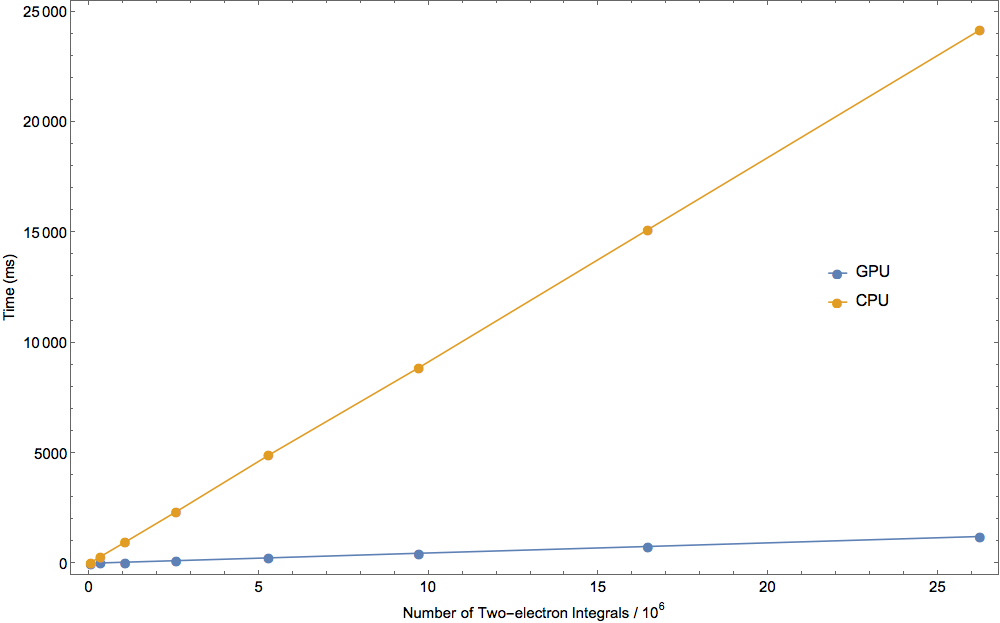
\includegraphics[width=1\textwidth]{Figures/eint2prof.png}
\caption[Profiling of two-electron integral calculations]
{Profiling of two-electron Integral calculations. The results of profiling the calculation of growing amounts of two-electron integrals. The blue line shows the time needed for GPU calculations and the yellow line shows time needed for CPU calculations. The time for the GPU calculations is the combined time of the \kernel{eint2} and \kernel{binary\_search} kernels.}
\label{fig:2eintprof}
\end{figure}

As can be seen, the GPU calculations of the two-electron integrals outperform the CPU calculations with an average speedup factor of over 19. For calculations with fewer number of integrals to compute the speedup is not as dramatic. This is most likely due to the overhead involved in just starting a GPU kernel. Table \ref{tab:2eintprof} shows two different speedups: one for just calculation of the integrals, and one that shows the speedup if the time needed for \kernel{binary\_search} is included. The time needed to evaluate indices does not have much of an impact on the total performance on the total calculation time which proves this was a good way to generate the $lmpqrs$ indices. Additionally, because cudaDFRATOM is a basis set optimizer, \kernel{binary\_search} will need to be called only once, whereas \kernel{eint2} may need to be called many hundreds of times. Therefore, for an optimization calculation (which the original program is incapable of doing) the total speedup will limit to the just the integral calculations.

\subsection{P and Q Matrix Formation Performance}
As explained in section \ref{sec:PQmeth}, there were two different attempts to speedup the formation of \textbf{P} and \textbf{Q}. The results of these attempts are shown in Tables \ref{tab:PQprofalg1} and \ref{tab:PQprofalg2} and also in Figure \ref{fig:formpqprof}.

\begin{table}[h!]
\begin{center}
\caption[\kernel{MTSE} kernel profiling results.]{\kernel{MTSE} kernel profiling results. Times are in ms. Times are given as the average time needed for a singel iteration from one calculation.}
\label{tab:PQprofalg1}
\begin{tabular}{rrrr}
\toprule
	Two-Electron Integrals	&	Time per Iteration CPU	&	Time per Iteration GPU	&	Speedup	\\
\midrule
	74305	&	1.90		&	6.06		&	0.31		\\
	353220	&	5.78		&	14.25	&	0.40		\\
	1081185	&	18.42	&	27.81	&	0.66		\\
	2588950	&	39.47	&	53.95	&	0.73		\\
	5299140	&	81.05	&	96.13	&	0.84		\\
	9726255	&	152.50	&	173.64	&	0.87		\\
	16476670	&	266.53	&	291.79	&	0.91		\\
	26248635	&	426.25	&	459.38	&	0.92		\\
\bottomrule
\end{tabular}
\end{center}
\end{table}

\begin{table}[h!]
\begin{center}
\caption[\kernel{STSE} kernel profiling results.]{\kernel{STSE} kernel profiling results. Times are in ms. Times are given as the average time needed for a singel iteration from one calculation.}
\label{tab:PQprofalg2}
\begin{tabular}{rrrr}
\toprule
	Two-Electron Integrals	&	Time per Iteration CPU		&	Time per Iteration GPU	&	Speedup	\\
\midrule
	74305	&	1.90		&	2.94		&	0.64	\\
	353220	&	5.78		&	7.56		&	0.76	\\
	1081185	&	18.42	&	15.34	&	1.20	\\
	2588950	&	39.47	&	26.32	&	1.49	\\
	5299140	&	81.05	&	39.45	&	2.05	\\
	9726255	&	152.50	&	88.78	&	1.71	\\
	16476670	&	266.53	&	135.64	&	1.96	\\
	26248635	&	426.25	&	193.99	&	2.19	\\
\bottomrule
\end{tabular}
\end{center}
\end{table}

\begin{figure}[h!]
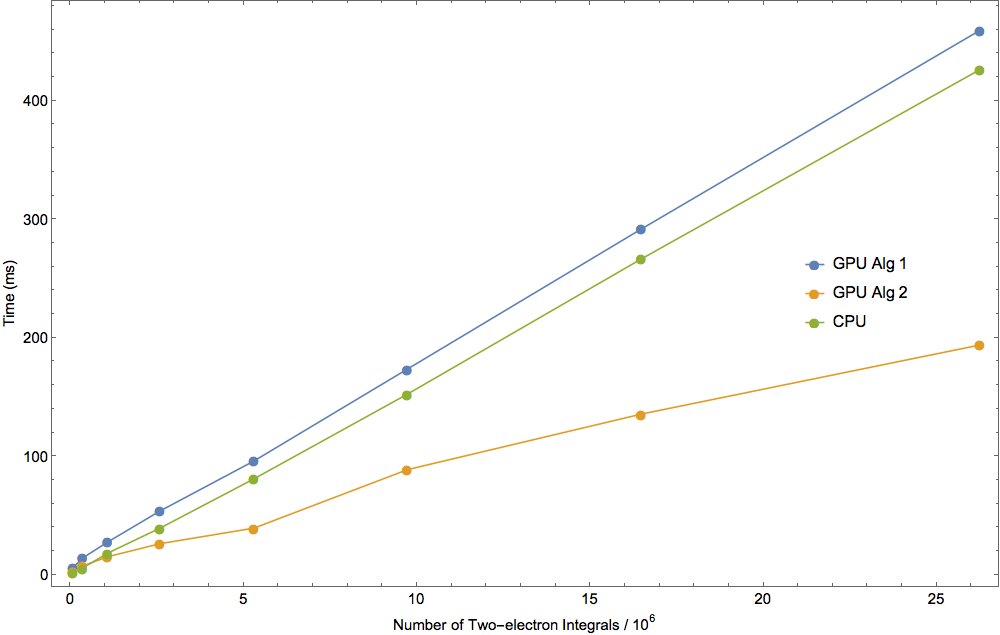
\includegraphics[width=1\textwidth]{Figures/formpqprof.png}
\caption[Profiling of the \kernel{formpq} kernels.]
{Profiling of the \kernel{formpq} kernels. The results of profiling the formation of the \textbf{P} and \textbf{Q} matrices. The blue line shows the time needed for GPU calculations using the \kernel{MTSE} algorithm, the yellow line shows time needed for GPU calculations using \kernel{STSE}, and the green line shows the time needed for the CPU. Because the GPU calculations converge in fewer SCF iterations than the CPU calculations, only the average time for one iteration is shown.}
\label{fig:formpqprof}
\end{figure}

As can be seen, the attempt at \kernel{MTSE} was a complete failure and it isn't even faster than the CPU calculations. \kernel{STSE} was much better, but only just. It achieves little more than a two-fold speedup at best. 

There are several reasons this could be the case. The first due to the poor global memory access that reading $x$ has. $x$ is stored as a vector. This helps greatly with memory cost and integral calculation, but makes it difficult to retrieve it as if it were a matrix.There is the cost of calculating where the necessary integral is, and then the cost of the very uncoalesced reads. Calculating the integrals as a vector, and then copying them into a matrix afterwards could help with this, but the large amount of integrals needed for large calculations makes this impractical on current hardware. How much of an effect inefficient access of global memory has on a calculation does have a limit however which is most likely why the speedup sees an improvement as the calculations get larger. A second reason that the speedup is limited is caused by the occupancy that the kernels can achieve on the GPU. A block size of 512 means that there is a maximum number of 3 blocks running per SM at a time. But these kernels are both limited by the register usage to just running one block per SM at a time. This is also most likely why \kernel{MTSE} performs so poorly compared \kernel{STSE}. \kernel{MTSE} was designed to spread out the amount of work to as many threads as possible. This results in a lot of blocks to be run. But because the amount of blocks that can run at a time is so limited there is no chance to see an improvement. But in the case of \kernel{STSE}, there are a fewer number of blocks needing be be run, although each one needs to run for longer than those of \kernel{MTSE}. Overall \kernel{MTSE} comes out on top.

\begin{figure}
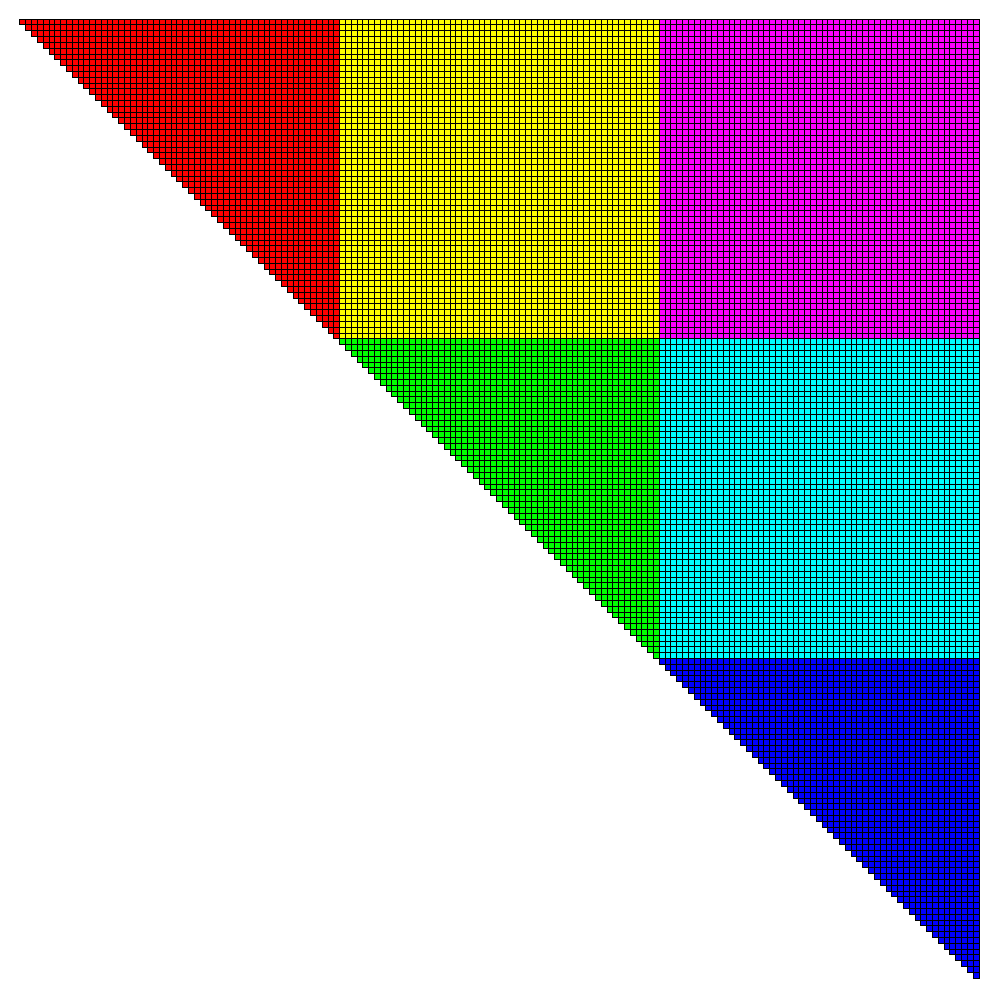
\includegraphics[width=1\textwidth]{Figures/eint2_mat_lots.png}
\caption[Integrals needed for the first element of \textbf{P}: matrix representation]
{Integrals needed for the first element of \textbf{P}: The top triangle of the symmetric two-electron integral matrix in a matrix representation. The required integrals have been highlighted with a green border. The basis set used had $nsym=3$ with $nbs(i) = (10, 10, 10)$. For clarity, the boxes have been coloured based on the spinor symmetries that they contain.}
\label{fig:eint2matlots}
\end{figure}

\begin{figure}
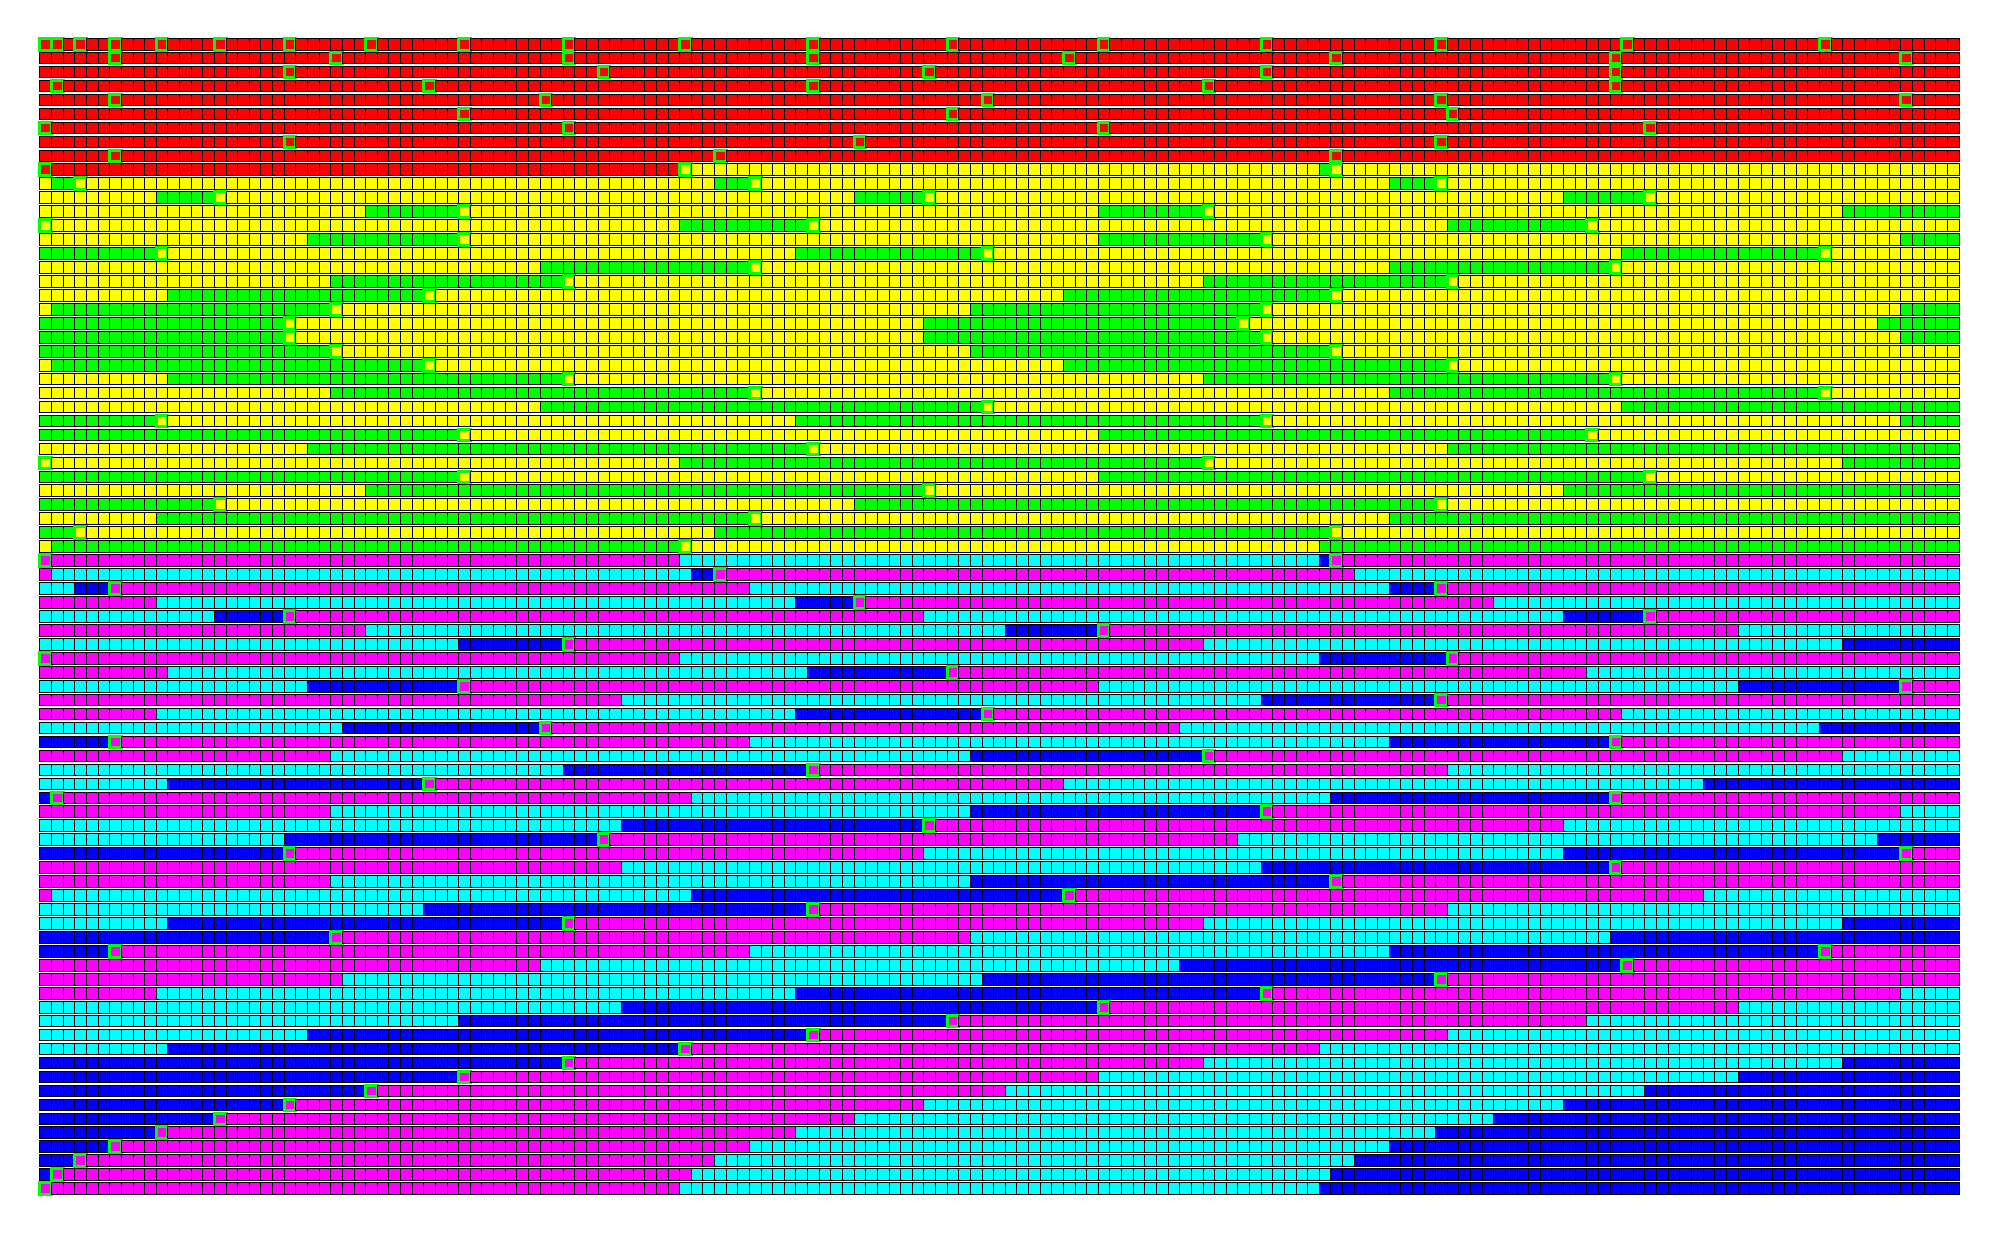
\includegraphics[width=1\textwidth]{Figures/eint2_vec_lots.png}
\caption[Integrals needed for the first element of \textbf{P}: vector representation]
{Integrals needed for the first element of \textbf{P}: The top triangle of the symmetric two-electron integral matrix in a vector representation. The required integrals have been highlighted with a green border.  The spreading out of the elements means that reads to them can not be done effectively. The basis set used had $nsym=3$ with $nbs(i) = (10, 10, 10)$. For clarity, the boxes have been coloured in the same way as Figure \ref{fig:eint2matlots}.}
\label{fig:eint2veclots}
\end{figure}


At present, the limitations of these algorithms are caused by the hardware they run on, not the efficiency of the algorithms themselves. If we imagine removing these limitations, we could consider which one will be better. I propose that \kernel{MTSE} will eventually surpass \kernel{STSE} for very large systems for the following reasons: the time it takes for a single block of \kernel{MTSE} to run is mostly governed by how well it can read the $x$ vector. The effect of spreading out the elements has on memory bandwidth has a limit, once the elements are spread out enough, spreading them out further has no impact. Therefore there is a maximum amount of time it takes for a single block to run. The time for a single block of \kernel{STSE} on the other hand is controlled by both the efficiency of reading global memory \textit{and} the amount of two-electron integrals it must read though. So there is no limit to how long a block can take. Therefore, I predict that \kernel{MTSE} should be faster as the number of integrals becomes very large.

\subsection{Total Speedup}
There was some difficulty in determining the total speedup of a calculation. The reason why can be seen in Tables \ref{tab:totalprofalg1} and \ref{tab:totalprofalg2}.

\begin{table}[h!]
\begin{center}
\caption[Total speedup of alg1]{Total speedup of cudaDFRATOM using \textbf{MTSE}. The results for a total calculation are shown. All times are in s. Times are given as the average time needed for five calculations.}
\label{tab:totalprofalg1}
\begin{tabular}{rrrrrr}
\toprule
	\multirow{2}{3cm}{Two-Electron Integrals}	&	\multirow{2}{3cm}{SCF Iterations CPU}	&	\multirow{2}{2cm}{Total CPU Time}		&	\multirow{2}{3cm}{SCF Iteractions GPU}		&	\multirow{2}{2cm}{Total GPU Time}		&	\multirow{2}{*}{Speedup}	\\
	\\
\midrule
	74305	&	21	&	0.12		&	21	&	0.84	&	0.14	\\
	353220	&	19	&	0.49		&	19	&	1.19	&	0.41	\\
	1081185	&	19	&	1.44		&	19	&	1.75	&	0.82	\\
	2588950	&	19	&	3.38		&	19	&	2.58	&	1.30	\\
	5299140	&	19	&	6.78		&	19	&	3.80	&	1.78	\\
	9726255	&	24	&	13.29	&	19	&	5.77	&	2.30	\\
	16476670	&	26	&	23.23	&	19	&	8.60	&	2.69	\\
	26248635	&	24	&	35.63	&	19	&	12.5	&	2.82	\\
\bottomrule
\end{tabular}
\end{center}
\end{table}

\begin{table}[h!]
\begin{center}
\caption[Total speedup of alg2]{Total speedup of cudaDFRATOM using \textbf{STSE}. The results for a total calculation are shown. All times are in s.}
\label{tab:totalprofalg2}
\begin{tabular}{rrrrrr}
\toprule
	\multirow{2}{3cm}{Two-Electron Integrals}	&	\multirow{2}{3cm}{SCF Iterations CPU}	&	\multirow{2}{2cm}{Total CPU Time}		&	\multirow{2}{3cm}{SCF Iteractions GPU}		&	\multirow{2}{2cm}{Total GPU Time}		&	\multirow{2}{*}{Speedup}	\\
	\\
\midrule
	74305	&	21	&	0.12		&	21	&	0.78	&	0.15	\\
	353220	&	19	&	0.49		&	19	&	1.07	&	0.46	\\
	1081185	&	19	&	1.44		&	19	&	1.51	&	0.95	\\
	2588950	&	19	&	3.38		&	19	&	2.08	&	1.62	\\
	5299140	&	19	&	6.78		&	19	&	2.72	&	2.49	\\
	9726255	&	24	&	13.29	&	19	&	4.14	&	3.20	\\
	16476670	&	26	&	23.23	&	19	&	5.57	&	4.16	\\
	26248635	&	24	&	35.63	&	19	&	7.47	&	4.76	\\
\bottomrule
\end{tabular}
\end{center}
\end{table}

\begin{figure}[h!]
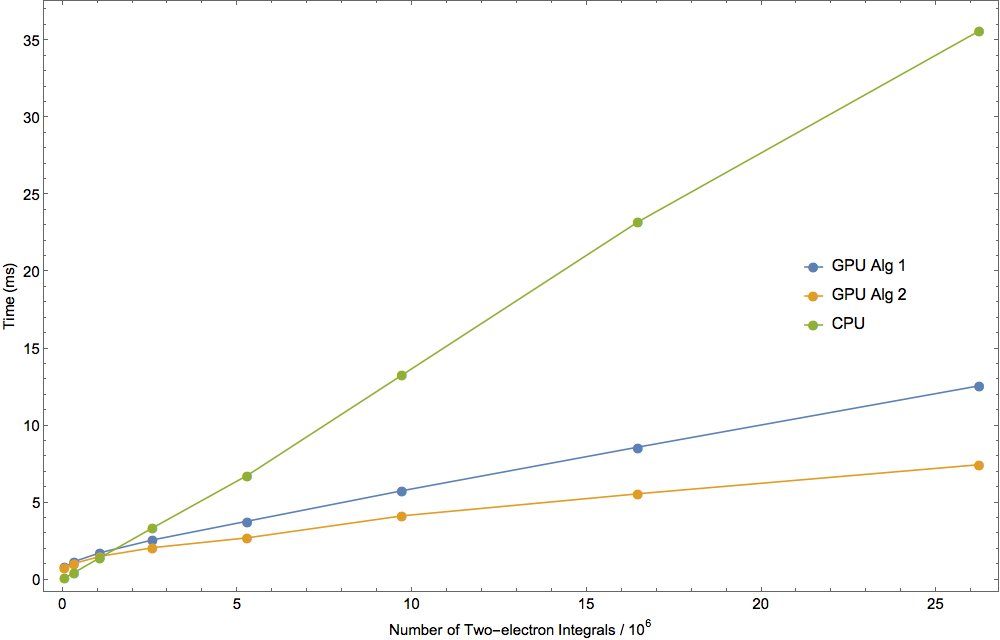
\includegraphics[width=1\textwidth]{Figures/totaltimeprof.png}
\caption[Total time need to complete a calculation.]
{Total time need to complete a calculation.}
\label{fig:totaltimeprof}
\end{figure}

As can be seen, the number of SCF iterations differs when comparing the GPU calculations to the CPU even though the convergence criteria was exactly the same. This is somewhat puzzling but I offer the following explanation. The differences do not occur in the two-electron integral calculations. We confirmed this by comparing the sum of the absolute values of the integrals from both the GPU and non-GPU programs and found that they were the same. The problem instead occurs as a result of changing the SCF routines. First, when writing the SCF routines, it became apparent that rewriting the linear algebra into CUDA would be rather pointless when I could just use the cuSOLVER and cuBLAS libraries and achieve the same result. As such, the SCF is completed using entirely different algorithms and unfortunately, these GPU libraries do not produce exactly the same eigenvalues as the original program. Second, it is important to realize that a real number can only be \textit{approximated} using double precision variables. This introduces numerical instability. For instance, assume that we have a computer that could only hold the first four digits of a number (leading zeros don't count). Then we take the number 1.000 and we want to add 0.0001000 to it 10000 times. The result of the first addition should be 1.0001, but because our computer can only hold four digits, the number is truncated to 1.000. The final result of this computation would not be 2.000 as expected but 1.000. During an SCF calculation, there are millions of numbers being multiplied together and added up, many of which may be close to, but not quite 0. This allows for lots of error to creep into a calculation just because of the limitations of the hardware. 

The fact that two different algorithms are being used on the GPU and CPU, and that they might not be handling numerical stability in the same way is what is most likely causing this to occur. It should also be pointed out that the final energy was not exactly the same from GPU to CPU either. Typically, the last 4 of 16 significant digits would be different. Because the rest are the same however, we still have ``chemical accuracy" (the general consensus of chemical accuracy is $0.001$ Hartree, which cudaDFRATOM falls well within) and I argue that cudaDFRATOMs results are therefore valid.


\section{Input Description}\label{inp_des}
cudaDFRATOM can be executed on Unix-like systems in the following way
\begin{lstlisting}[language=bash]
	$ path_to_executable input_file > output_file
\end{lstlisting}

The input file must end in ``.inp" or an error will be given. Redirection of stdout to an output file is optional, but is recommended to save the results of a calculation. The input file is read using the namelist functionality of Fortran. A description of what must appear on each line of the input file is given below. Sample input files are also given in Appendix \ref{app:cudaDFRATOM_inp}.

\begin{enumerate}
	\item A title of no more than 200 characters.
	\item	\$contrl	\\
				\\
		\begin{tabular}{\vartables}
			jobtype	&		&			&	The type of calculation to be performed.							\\
					&	=	& 	'energy'	& 	Will do a single point energy calculation.							\\
					&	=	&	'bsopt'	& 	Will optimize the basis set. Can only be used if bastype equals 'wtbs'.	\\
			c		&		&			&	The speed of light. If not given, the default is set to 137.03599976 au.	\\
		\end{tabular}
	\item \$nuc	\\
				\\
		\begin{tabular}{\vartables}
			znuc		&		&		&	The charge of the nucleus.									\\
			nucmdl	&		& 		&	The nuclear model to use.										\\
					&	=	&	1	&	Point nucleus (default).										\\
					&	=	&	2	&	Finite sphere (not yet supported). 								\\
					&	=	&	3	&	Gaussian.													\\
			rnuc		&		&		&	The radius of the finite sphere nucleus.							\\	
			alpha	&		&		&	The exponent for the gaussian nucleus. Defaults are given in litdata.f90.	\\				
		\end{tabular}
	\item \$bas	\\
				\\
			\begin{tabular}{\vartables}
			nsym	&		&			&	The number of symmetries to be used.							\\
			bastype	&		& 			&	The type of basis set given.									\\
					&	=	&	'wtbs'	&	Use a WTBS basis set.										\\
					&	=	&	'rdin'		&	Read in the basis set from the input file.							\\
			ngroup	&		&			&	The number of different groups to use in the WTBS scheme (default 1).	\\			
		\end{tabular}
		\\			
		The next line will depend on the value of bastype. If bastype equals `rdin' then the following lines must be the number of functions for the S+ symmetry, followed by the exponents to use, each on a new line. The pattern repeats for each new symmetry. See the sample input files for further clarification. Otherwise, if bastype equals `WTBS' the \$wtbs group is read next.
		
	\item \$wtbs has to be given if bastype='wtbs'.	\\
										\\
		\begin{tabular}{\vartables}
			wtbspara	&		&	&	The $\alpha$, $\beta$, $\delta$, and $\gamma$ WTBS parameters.
									If there is more than one group, the order would be  $\alpha_{1}$, $\beta_{1}$, 
									$\delta_{1}$, $\gamma_{1}$,  $\alpha_{2}$, $\beta_{2}$, $\delta_{2}$, $\gamma_{2}$ 
									and so on.																	\\
			nbs		&		& 	&	The number of functions used in each symmetry.									\\
			start		&		&	&	Where in the $\zeta$ pool each symmetry starts taking exponents from (default=1,1,1,1,1,1,1).	\\
			groups	&		&	&	What group each symmetry belongs to (default=1,1,1,1,1,1,1).							\\
		\end{tabular}
		\\
		The next line depends on what the jobtype was set to. If jobtype equals 'energy' \$newuoa is skipped and \$econfig will be read next. If jobtype equals `bsopt', then the \$newuoa group will be needed.
		
		\item \$newuoa has to be given if jobtype='bsopt'. Refer to the newuoa documentation \cite{Powell2006} for detailed information if needed.	\\
												\\
		\begin{tabular}{\vartables}
			rhobeg	&		&		&	The initial value of the trust region used by newuoa (default=0.1).									\\
			rhoend	&		& 		&	The final value of the trust region used by newuoa. Must be smaller
										than rhobeg (default=$1.0\times{}10^{-4}$).			\\
			iprint		&		&		&	The print level for newuoa.													\\
					&	=	&	0	&	No printing from newuoa (default).												\\
					&	=	&	1	&	Print only when newuoa has finished.											\\
					&	=	&	2	&	Print only when the trust region has decreased by an order of magnitude.					\\
					&	=	&	3	&	Print every iteration of newuoa.													\\
			maxfun	&		&		&	The maximum number of calls to calfun newuoa will make before terminating (default=500).	\\
		\end{tabular}
		\\
		\item \$econfig
		\\
		\begin{tabular}{\vartables}
			nclose	&		&		&	The number of closed spinors for each symmetry.										\\
			nopen	&		& 		&	The number of open spinors for each symmetry. There is a limit to one open orbital per symmetry.	\\
			freeel	&		&		&	The number of electrons available in the open spinors.									\\
			autogen	&		&		&	Automatically generates all possible combinations of spinor occupancies (default=.false.).			\\
			nconf	&		&		&	The number of configurations to be read in (needed if autogen is false).						\\
		\end{tabular}
		\\
		If autogen is false, then the next nconf lines will be the spinor occupancies. They will be given as real numbers with one configuration per line.
		\\
		\\
		\item \$scf
		\\
		\begin{tabular}{\vartables}
			maxitr	&		&		&	The maximum number of SCF iterations (default=50).									\\
			ixtrp		&		& 		&	The method of extrapolation.														\\
					&	=	&	0	&	No extrapolation (default).															\\
					&	=	&	1	&	Extrapolate the Fock matrix.														\\
			dfctr		&		&		&	Damping factor for Fock maxtrix (default=0.3).											\\
			thdll		&		&		&	Convergence limit for the large-large components of the density matrix (default=$1.0\times10^{-5}$)	\\
			thdsl		&		&		&	Convergence limit for the small-large components of the density matrix (default=$1.0\times10^{-7}$)	\\
			thdss	&		&		&	Convergence limit for the small-small components of the density matrix (default=$1.0\times10^{-9}$)	\\
		\end{tabular}
		\\
\end{enumerate}

\chapter{Basis Sets}
\label{chap:basis_sets}
\section{Introduction}
As stated in section \ref{subsec:basis_sets}, the use of Gaussian-type functions is the favored way of constructing basis sets for the use in molecular calculations. The use of basis sets introduces a new source of error, as we are now only approximating a wavefunction instead of directly numerically calculating it. One of the ways this error can manifest itself is in basis set superposition error (BSSE). BSSE appears when comparing the differences in energy between two different systems, as one might do to compare the difference in energy between reactants and product in a chemical reaction. 

\notetodylan{For instance, we might want to find the energy of the reaction $\text{H}^{+} + \text{OH}^{-} \rightarrow \text{H}_{2}\text{O}$. The calculation of $\text{H}_{2}\text{O}$ will have three basis functions centers while the $\text{OH}^{-}$ calculation will only have two. The $\text{OH}^{-}$ fragment inside the $\text{H}_{2}\text{O}$ molecule will have additional basis functions from the $\text{H}^{+}$ fragment to work with while the $\text{OH}^{-}$ does not. As a result, the $\text{OH}^{-}$ fragment and molecule are not being described exactly the same, and therefore errors can result from this.}

%Because we can not use a basis set with an infinite amount of basis functions, the basis set for the products and reactants in this example will be different (each will potentially have a different number of basis function centers, locations, etc.). This means that we are not comparing calculations with exactly the same level of accuracy, and the results may be invalidated because of this. 

There is also the possibility of approximate linear dependencies in the basis set, which may show up during the SCF process. This happens when the overlap between any two different functions is close to unity (at least as far as a double precision number is concerned) and will mean that there will be eigenvalues that are equal to zero when diagonalizing the overlap matrix. We cannot find the inverse of such a matrix, so therefore the functions leading to these eigenvalues of zero must get transformed out of the matrix. This is kind of bandaid solution though, as the resulting Fock matrix after this transformation could produce errors in the energy differences on the order of chemical accuracy. It can also lead to a very aggravating process during a geometry optimization. 

For example, say we have a molecular system in geometry state A. In this state, there are no approximate linear dependencies, and the geometry optimizer determines that the system would prefer to be in geometry state B. It updates the geometry, but in state B, some atoms might be too close together and now there are eigenfunctions that need to be rejected. The energy calculated for geometry state B is inaccurate, which causes the geometry optimizer to think that it should place the atoms back into state A. But now, everything is exactly the same as it was, and the geometry optimizer, with no memory at all of what just happened, thinks that the perfect geometry is state B again. There is no way out of this loop, and we will not be able to find a stationary state, and all because of a poor choice in basis set. It is therefore important for a computational chemist to be aware of these issues so they can identify them when they occur, but even more so for someone who wants to make a new basis set, so that these issues can be avoided in the first place.

Designing a basis set that reduces the effects of BSSE is relatively straightforward, we can simply brute force the problem by adding more and more functions until they begin to cancel each other out. Designing one that avoids the issue of approximate linear dependencies however is more tricky. It is simply not possible to test every possible combination of atoms in every possible geometry to determine if a basis set has these problems. But there are some strategies we can use to avoid this problem.

One strategy that has shown to be particularly effective is using an exponent generating function to ensure that the exponents of the basis set are sufficiently different. There are many of these generating functions. One of these give what are called even-tempered basis sets (ETBS)\cite{ETBS}. The generating function for an ETBS is given below

\begin{equation}
\label{eq:ETBS_gen}
\zeta_{l,k} = \alpha_{l}\beta^{k-1}_{l}, \quad \alpha_{l}, \beta_{l} > 0, \quad \beta_{l} \neq 1, \quad k = 1, 2, \ldots
\end{equation}

where $\zeta_{l,k}$ is the $k^{\text{th}}$ exponent of basis function for orbital symmetry $l$, $\alpha_{l}$ is the exponent for the first, most diffuse, basis function, and $\beta_{l}$ is a growth parameter that determines the gap between $\zeta_{l,k}$ and $\zeta_{l,k + 1}$. This greatly reduces the difficulty of the problem, because instead of needing to optimize all the exponents of our basis set, we only need to optimize the $\alpha$ and $\beta$ parameters of each symmetry. We can further reduce the number of parameters to optimize by using the same $\alpha$ and $\beta$ parameters \textit{for each symmetry}. This is what I did for the work in this chapter, so I will drop the $l$ subscript. However, there is a problem with ETBS: the growth in the value of the exponents is not always sufficient. So we get diminishing returns by increasing the maximum value of $k$, and we have to add many more functions to improve the accuracy of the basis set by even a small amount. This is improved in the well-tempered basis set (WTBS)\cite{WTBS} generating function, which is shown below

\begin{equation}
\label{eq:WTBS_gen}
\zeta_{k} = \zeta_{k-1}\beta\left[1+\gamma\left(\frac{k}{n}\right)^{\delta}\right], \quad k = 2, 3,\ldots, n, \quad \zeta_{1}=\alpha
\end{equation}

where $n$ is the maximum number of basis functions for the set, and $\alpha$ and $\beta$ have the same restrictions on them as they did before. The parameters $\delta$ and $\gamma$ have the effect of increasing the gap between $\zeta$s caused by $\beta$ at high $k$. This means that the growth of the exponents is increased as they get larger, which allows them to make a more meaningful contribution to the total wavefunction. Thus, we get a more accurate basis set with far fewer functions. The effect that altering $\gamma$ and $\delta$ has on the exponents can be seen in Figure \ref{fig:deltagamm}.

\begin{figure}
\center
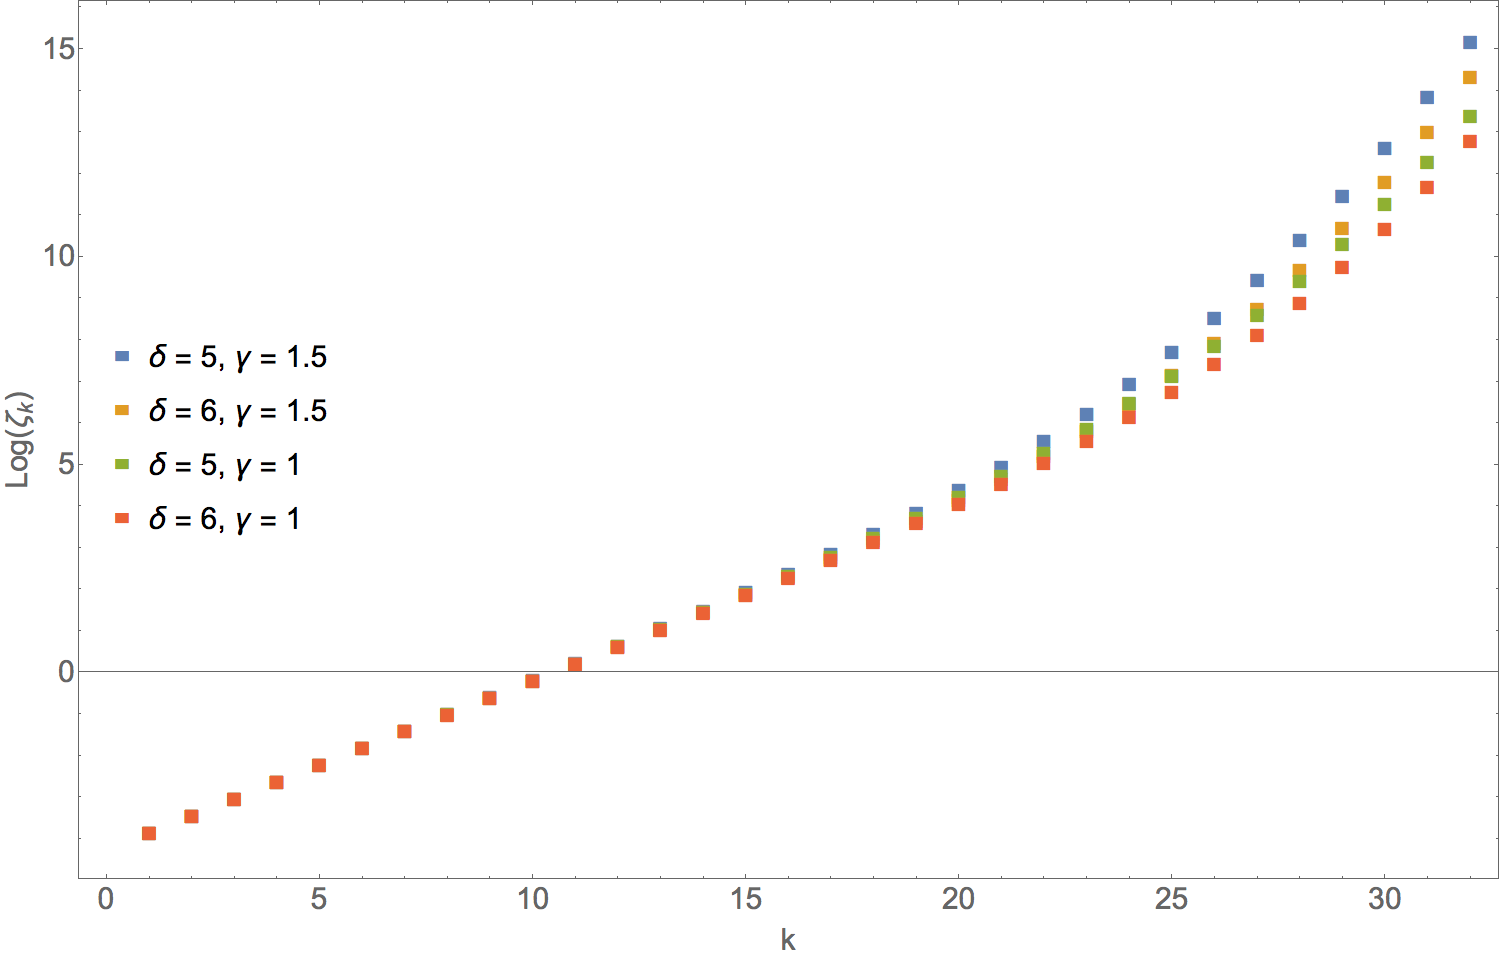
\includegraphics[width=1\textwidth]{Figures/deltagamm.png}
\caption[Changes in $\zeta$ as the values of $\delta$ and $\gamma$ are changed.]
{Changes in $\zeta$ as the values of $\delta$ and $\gamma$ are changed. The value of $n$ was 36, $\alpha$ was 0.02, and $\beta$ was 1.5}
\label{fig:deltagamm}
\end{figure}

It should be mentioned that each symmetry does not need to use the entire set of $\zeta$s that we optimize. Indeed, the most diffuse orbitals in the valence shells often don't use the most contracted functions at all, and conversely the most contracted orbitals in the core don't make much use of the most diffuse functions. Therefore, it is better to think of the set of $\zeta$s as pool, and that each symmetry is drawing a range of functions from that pool.  

\section{Methods}
\subsection{Basis set size optimization}
We decided to use a somewhat novel method of generating our basis sets. We begin by choosing an arbitrarily large basis set size, such as \mbox{s$(1:40)$p$(1:40)$d$(1:40)$f$(1:40)$} (here $i(\#:\#)$ refers to the starting and ending index of $\zeta$'s used for symmetry $i$). Next, we then find the optimal $\alpha$, $\beta$, $\delta$, and $\gamma$ WTBS parameters for this basis set. \notetodylan{This is done using NEWUOA\cite{Powell2006} which finds the values $\alpha$, $\beta$, $\delta$, and $\gamma$ that lead to the lowest possible energy for a given basis set size.} Finally, we use the following steps to find the optimal basis set size.

\textit{Step 1.} Begin by finding the fewest number of f functions necessary. This can be done by generating input files that range in size from  \mbox{s$(1:40)$p$(1:40)$d$(1:40)$f$(1:1)$} to  \mbox{s$(1:40)$p$(1:40)$d$(1:40)$f$(1:40)$}.

\textit{Step 2.} Optimize the basis sets and select the smallest basis set that is still below some minimum accuracy threshold. We chose a relative error to numerical calculations of no greater than $5.0\times10^{-9}$ for non-relativistic sets and $5.0\times10^{-8}$ for relativistic sets where relative error is defined as $\frac{|(\text{optimized energy}) - (\text{numerical energy})|}{\text{numerical energy}}$. The size of this basis set is  \mbox{s$(1:40)$p$(1:40)$d$(1:40)$f$(1:x_{f})$}.

\textit{Step 3.} Replace the WTBS parameters with those from the newly optimized set and generate a list of input files that range in size from  \mbox{s$(1:40)$p$(1:40)$d$(1:x_{f})$f$(1:x_{f})$} to  \mbox{s$(1:40)$p$(1:40)$d$(1:40)$f$(1:x_{f})$}.

\textit{Step 4.} Optimize these new sets and select the smallest one that brings about an error that is still below the accuracy threshold. The size of this basis set is \\ \mbox{s$(1:40)$p$(1:40)$d$(1:x_{d})$f$(1:x_{f})$}.

\textit{Step 5.} Repeat steps 3 and 4 for the remaining symmetries. The size of the basis set at the end of this step will be of size  \mbox{s$(1:x_{s})$p$(1:x_{p})$d$(1:x_{d})$f$(1:x_{f})$}.

\textit{Step 6.} Replace the WTBS parameters with those from the newly optimized set and generate a list of input files that range in size from  \mbox{s$(1:x_{s})$p$(1:x_{p})$d$(1:x_{d})$f$(1:x_{f})$} to  \mbox{s$(1:x_{s})$p$(1:x_{p})$d$(1:x_{d})$f$(x_{f}:x_{f})$}.

\textit{Step 7.} Optimize and select from the basis sets. The new set will be of size  \\ \mbox{s$(1:x_{s})$p$(1:x_{p})$d$(1:x_{d})$f$(y_{f}:x_{f})$}.

\textit{Step 8.} Repeat steps 6 and 7 for the other symmetries except s. The final basis set will be of size  \mbox{s$(1:x_{s})$p$(y_{p}:x_{p})$d$(y_{d}:x_{d})$f$(y_{f}:x_{f})$}.

This procedure is perhaps a bit clunky, so let us work through an example using Ne. Ne has both s and p type orbitals, and so will our basis set. We might initially guess that no more than 26 functions per symmetry will enough to get the accuracy we want, so we start with a basis set of size s(1:26)p(1:26). We then optimize the $\alpha$, $\beta$, $\delta$, and $\gamma$ parameters for a basis set of this size. We make sure that the energy using a basis set of this size produces results that are accurate enough, and then we begin to reduce the size of the basis set for the p space. We carry over the WTBS parameters optimized in the last step, and generate input files corresponding to basis sets of size s(1:26)p(1:15) to s(1:26)p(1:26) (12 calculations in total) to determine the minimum number of tight functions we will need to accurately describe the p orbitals. After reoptimizing the WTBS parameters, we find that while s(1:26)p(1:15) is too small to be accurate enough, s(1:26)p(1:16) is still inside the threshold we want. So, we take the WTBS parameters from this calculation, and use them to generate new basis sets ranging in size from s(1:16)p(1:16) to s(1:26)p(1:16) (so we are trying to eliminate contracted functions from the s orbitals). Here we find that s(1:23)p(1:16) is the smallest basis set we can use. Now, we want to eliminate diffuse functions. Carrying over the WTBS parameter from the last acceptable basis set, we generate basis sets of size s(1:23)p(1:16) to s(1:23)p(5:16). We find that trying to remove any more functions makes the basis set unacceptable so we keep the s(1:23)p(1:16) basis set. We could try to remove diffuse functions from the s symmetry, but experience teaches that the s space needs all the functions to be accurate, so we don't bother.

This process has a major drawback in that it requires a lot of computer power to run efficiently. But this is not really a problem if access to large computer clusters is available. Additionally, considering that calculations for the chain 1-8 can be run in parallel for different atoms, this optimization process is trivially parallel. The advantages of this process are twofold: it finds a very small basis set that is still accurate and it is completely automatable. If there are no problems with individual calculations not converging, the output files never even need to be manually (and intellectually) examined! We generated non-relativistic basis sets for elements 2-86 using the rWTBS program\cite{WTBS, WTBS2, WTBS3, WTBS4, WTBS5, WTBS6} and relativistic basis sets for elements 55-86 using the cudaDFRATOM program which is outlined in detail in Chapter \ref{chp:cuda_dfratom}.

\subsection{Automating Optimization}
Automating the optimization process was quite simple. I did this by writing two scripts: BS\_sub\_auto\_rwtbs.sh and BS\_find\_best\_rwtbs.sh. The code for BS\_sub\_auto.sh is given here

\lstinputlisting[caption={BS\_sub\_auto\_rwtbs.sh},language=bash,framexrightmargin=15mm]{code_snippets/BS_sub_auto_rwtbs.sh}

The first few lines handle the arguments given to the script. The arguments are flags which tell the script what to do. The flags can be given in any order, so long as each flag is followed by the appropriate options. The default flag is a file ending in ``.inp" for the calculation that you would like to run. Optionally, this flag can be omitted, which will tell the script to run over all ``inp" files in the current directory. I will refer to the input file to be used as a seed. The flags ``-S", ``-P", ``-D", and ``-F" tell the script which set of orbitals we would like to remove functions from (``-S" means s orbitals, ``-P" means p orbitals, and so on). These flags \textit{\underline{must}} be followed by by two integers, with the first being smaller than the second. The first number is the minimum number for functions to cut, and the second is the maximum number to cut. By default, cutting begins with the most contracted function. For example, using ``-S 0 3" would take the seed file with a basis set of size s(1:20) and produce otherwise identical files with basis sets of size s(1:20), s(1:19), s(1:18), and s(1:17). If the number are negative, this can be used to add basis functions (``-S -1 0" on the same seed would produce basis sets of size s(1:21) and s(1:20)). Using the ``-B" (for bottom) flag changes the default behavior of cutting contracted functions, to cutting diffuse functions. So for example, using the flags ``-S 0 3 -B" on the seed would produce s(1:20), s(2:20), s(3:20), and s(4:20).

Once the flags have been parsed, the script makes a directory with the same name as the title of the seed, moves inside this directory, and generates the needed input files. It also creates a job submission script using the boilerplate function for each of new input files and submits them. Note that this part of the script will need to be changed depending on the cluster it is being used on. If more than one seed is used, then the script will do the same thing for each seed. After the jobs are completed, the user runs BS\_find\_best\_rwtbs.sh in the directory that contains all of the newly created directories. The code for BS\_find\_best\_rwtbs.sh is given below

\lstinputlisting[caption={BS\_find\_best\_rwtbs.sh},language=bash]{code_snippets/BS_find_best.sh}

This script takes in one argument, the relative error we are looking for in a calculation. It enters each of the subdirectories made by BS\_sub\_auto.sh and scans the output files for the relative error compared to numerical calculations. It finds the file with the smallest basis set that is still under the error threshold, and copies the input and output files for that calculation into a new directory called ``best". The user can then repeat this process for as many orbitals as they wish. There are also similar scripts for cudaDFRATOM which are given in Appendix \ref{app:cuda_dfratom_scripts}.

\section{Discussion}
\subsection{Optimized Non-Relativistic Basis Sets}
The optimized non-relativistic WTBS parameters and basis set sizes for elements 2-86 are shown in Table \ref{tab:BStab}. Relativistic WTBS parameters for elements 55-86 are shown in Table \ref{tab:BStab_rel}. Table \ref{tab:BStab_with_refs} gives the energies calculated with these basis sets compared to their literature values.

\begin{longtable}{l l r r r r r r r r}
\caption[Basis sets optimized using rWTBS]{Basis sets optimized using rWTBS. We did not have literature data for some elements. These elements are marked with a *. The size of the basis set for these elements was determined by using the size of the nearest elements.}\label{tab:BStab} \\
\toprule
	Element	&	Term		&	$\alpha$	&	$\beta$	&	$\delta$	&	$\gamma$	&	s	&	p	&	d	&	f	\\
			&	Symbol	&			&			&			&				&		&		&		&		\\
\midrule
\endfirsthead
\caption[]{(continued)}\\
\toprule
	Element	&	Term		&	$\alpha$	&	$\beta$	&	$\delta$	&	$\gamma$	&	s	&	p	&	d	&	f	\\
			&	Symbol	&			&			&			&				&		&		&		&		\\
\midrule
\endhead
02 He	& 	$^{1}S$  	&   	8.140$\times10^{-2}$   	&    	1.953    	&    	4.504    	&    	1.515    	&    	(1:18)    	\\
03 Li 	& 	$^{2}S$  	&   	1.596$\times10^{-2}$   	&    	1.933    	&    	5.701    	&    	1.573    	&    	(1:22)    	\\
04 Be 	& 	$^{1}S$  	&   	2.647$\times10^{-2}$   	&    	1.938    	&    	5.841    	&    	1.594    	&    	(1:22)    	\\	
05 B 		& 	$^{2}P$  	&   	3.238$\times10^{-2}$   	&    	1.948    	&    	5.573    	&    	1.523    	&    	(1:22)    	&    	(1:15)    	\\
06 C 	&  	$^{3}P$  	&   	4.613$\times10^{-2}$   	&    	1.941    	&    	4.717    	&    	1.317    	&    	(1:23)    	&    	(1:15)    	\\
07 N 	&  	$^{4}S$  	&   	5.976$\times10^{-2}$   	&    	1.923    	&    	5.183    	&    	1.442    	&    	(1:23)    	&    	(1:16)    	 \\
08 O 	&  	$^{3}P$  	&   	6.967$\times10^{-2}$   	&    	1.936    	&    	5.170    	&    	1.426    	&    	(1:23)    	&    	(1:16)    	\\
09 F 		&  	$^{2}P$  	&   	8.321$\times10^{-2}$   	&    	1.942    	&    	5.084    	&    	1.408    	&    	(1:23)    	&    	(1:16)    	\\
10 Ne 	&  	$^{1}S$  	&   	9.943$\times10^{-2}$   	&    	1.945    	&    	4.988    	&    	1.392    	&    	(1:23)    	&    	(1:16)    	\\
11 Na 	&  	$^{2}S$  	&   	1.696$\times10^{-2}$   	&    	1.950    	&    	6.056    	&    	1.469    	&    	(1:26)    	&    	(3:19)    	 \\
12 Mg 	&  	$^{1}S$  	&   	2.375$\times10^{-2}$   	&    	1.932    	&    	5.686    	&    	1.430    	&    	(1:26)    	&    	(3:19)    	\\
13 Al 	&  	$^{2}P$  	&   	2.239$\times10^{-2}$   	&    	1.898    	&    	5.555    	&    	1.413    	&    	(1:27)    	&    	(1:20)    	 \\
14 Si 	&  	$^{3}P$  	&   	3.352$\times10^{-2}$   	&    	1.921    	&    	5.419    	&    	1.410    	&    	(1:26)    	&    	(1:19)    	 \\
15 P 		&  	$^{4}S$  	&   	4.410$\times10^{-2}$   	&    	1.907    	&    	5.196    	&    	1.390    	&    	(1:26)    	&    	(1:19)    	    \\
16 S 		&  	$^{3}P$  	&   	5.004$\times10^{-2}$   	&    	1.896    	&    	4.962    	&    	1.362    	&    	(1:26)    	&    	(1:19)    	    \\
17 Cl 	&  	$^{2}P$  	&   	5.831$\times10^{-2}$   	&    	1.886    	&    	4.784    	&    	1.344    	&    	(1:26)    	&    	(1:19)    	    \\
18 Ar 	&  	$^{1}S$   	&   	6.834$\times10^{-2}$   	&    	1.878    	&    	4.654    	&    	1.331    	&    	(1:26)    	&    	(1:19)    	    \\
19 K 		&  	$^{2}S$   	&   	1.392$\times10^{-2}$   	&    	1.889    	&    	6.354    	&    	1.523    	&    	(1:28)    	&    	(3:22)    	    \\
20 Ca 	&  	$^{1}S$   	&   	1.837$\times10^{-2}$   	&    	1.874    	&    	6.109    	&    	1.504    	&    	(1:28)    	&    	(3:22)    	    \\
21 Sc 	&  	$^{2}D$   	&   	2.040$\times10^{-2}$   	&    	1.878    	&    	6.160    	&    	1.505    	&    	(1:28)    	&    	(3:22)    	&    	(2:16)   \\
22 Ti 	&  	$^{3}F$   	&   	2.218$\times10^{-2}$   	&    	1.886    	&    	6.247    	&    	1.508    	&    	(1:28)    	&    	(3:22)    	&    	(2:16)   \\
23 V 		&  	$^{4}F$   	&   	2.361$\times10^{-2}$   	&    	1.887    	&    	6.573    	&    	1.507    	&    	(1:29)    	&    	(3:23)    	&    	(2:16)   \\
24 Cr 	&  	$^{7}S$   	&   	2.345$\times10^{-2}$   	&    	1.865    	&    	5.348    	&    	1.407    	&    	(1:29)    	&    	(3:22)    	&    	(2:17)   \\
25 Mn 	&  	$^{6}S$   	&   	2.572$\times10^{-2}$   	&    	1.865    	&    	5.336    	&    	1.407    	&    	(1:29)    	&    	(3:22)    	&    	(2:17)   \\
26 Fe 	&  	$^{5}D$   	&   	2.621$\times10^{-2}$   	&    	1.869    	&    	5.301    	&    	1.395    	&    	(1:29)    	&    	(3:22)    	&    	(3:17)   \\
27 Co 	&  	$^{4}F$   	&   	2.643$\times10^{-2}$   	&    	1.871    	&    	5.905    	&    	1.413    	&    	(1:29)    	&    	(4:23)    	&    	(3:17)   \\
28 Ni 	&  	$^{3}F$   	&   	2.882$\times10^{-2}$   	&    	1.875    	&    	5.935    	&    	1.413    	&    	(1:29)    	&    	(3:23)    	&    	(3:17)   \\
29 Cu 	&  	$^{2}S$   	&   	2.283$\times10^{-2}$   	&    	1.857    	&    	5.485    	&    	1.413    	&    	(1:30)    	&    	(4:23)    	&    	(3:18)   \\
30 Zn 	&  	$^{1}S$   	&   	3.297$\times10^{-2}$   	&    	1.881    	&    	5.817    	&    	1.339    	&    	(1:30)    	&    	(3:24)    	&    	(2:17)   \\
31 Ga 	&  	$^{2}P$   	&   	2.742$\times10^{-2}$   	&    	1.863    	&    	5.703    	&    	1.462    	&    	(1:30)    	&    	(1:23)    	&    	(3:18)   \\
32 Ge 	&  	$^{3}P$   	&   	3.143$\times10^{-2}$   	&    	1.848    	&    	5.290    	&    	1.386    	&    	(1:30)    	&    	(1:23)    	&    	(4:18)   \\
33 As 	&  	$^{4}S$   	&   	4.728$\times10^{-2}$   	&    	1.869    	&    	5.325    	&    	1.340    	&    	(1:30)    	&    	(1:23)    	&    	(3:17)   \\
34 Se 	&	$^{3}P$   	&   	5.087$\times10^{-2}$   	&    	1.847    	&    	4.949    	&    	1.533    	&    	(1:30)    	&    	(1:22)    	&    	(3:18)   \\
35 Br 	&  	$^{2}P$   	&   	5.927$\times10^{-2}$   	&    	1.861    	&    	5.192    	&    	1.333    	&    	(1:30)    	&    	(1:23)    	&    	(3:17)   \\
36 Kr 	&  	$^{1}S$   	&   	6.804$\times10^{-2}$   	&    	1.859    	&    	5.510    	&    	1.370    	&    	(1:29)    	&    	(1:23)    	&    	(3:17)   \\
37 Rb 	&  	$^{2}S$   	&   	1.421$\times10^{-2}$   	&    	1.856    	&    	7.181    	&    	1.626    	&    	(1:30)    	&    	(3:25)    	&    	(6:21)   \\
38 Sr 	&  	$^{1}S$   	&   	1.808$\times10^{-2}$   	&    	1.846    	&    	6.674    	&    	1.553    	&    	(1:30)    	&    	(3:25)    	&    	(6:20)   \\
39 Y 		&  	$^{2}D$   	&   	1.997$\times10^{-2}$   	&    	1.841    	&    	6.569    	&    	1.543    	&    	(1:30)    	&    	(3:25)    	&    	(2:20)   \\
40 Zr 	&  	$^{5}F$   	&   	2.184$\times10^{-2}$   	&    	1.837    	&    	6.485    	&    	1.535    	&    	(1:30)    	&    	(3:25)    	&    	(2:20)   \\
41 Nb 	&  	$^{6}D$   	&   	2.340$\times10^{-2}$   	&    	1.835    	&    	6.434    	&    	1.530    	&    	(1:30)    	&    	(3:25)    	&    	(2:20)   \\
42 Mo 	&  	$^{7}S$   	&   	2.537$\times10^{-2}$   	&    	1.832    	&    	6.372    	&    	1.524    	&    	(1:30)    	&    	(3:25)    	&    	(2:20)   \\
43 Tc 	&  	$^{6}S$   	&   	2.597$\times10^{-2}$   	&    	1.836    	&    	6.453    	&    	1.534    	&    	(1:30)    	&    	(3:25)    	&    	(2:20)   \\
44 Ru 	&  	$^{5}F$   	&   	2.682$\times10^{-2}$   	&    	1.833    	&    	6.788    	&    	1.606    	&    	(1:30)    	&    	(3:25)    	&    	(2:21)   \\
45 Rh 	&  	$^{4}F$   	&   	2.751$\times10^{-2}$   	&    	1.835    	&    	6.883    	&    	1.620    	&    	(1:30)    	&    	(3:25)    	&    	(2:21)   \\
46 Pd 	&  	$^{1}S$   	&   	5.944$\times10^{-2}$   	&    	1.827    	&    	5.980    	&    	1.504    	&    	(1:29)    	&    	(2:24)    	&    	(1:19)   \\
47 Ag 	&  	$^{2}S$   	&   	2.438$\times10^{-2}$   	&    	1.800    	&    	5.521    	&    	1.423    	&    	(1:31)    	&    	(4:25)    	&    	(3:21)   \\
48 Cd 	&  	$^{1}S$   	&   	2.911$\times10^{-2}$   	&   	1.786   	&   	5.334   	&   	1.408   	&   	(1:31)   	&    	(4:25)    	&    	(3:21)   \\
49 In 	&  	$^{2}P$   	&   	2.714$\times10^{-2}$   	&    	1.799    	&    	5.540    	&    	1.431    	&    	(1:31)    	&    	(1:25)    	&    	(3:21)   \\
50 Sn 	&  	$^{3}P$   	&   	2.884$\times10^{-2}$   	&    	1.794    	&    	5.422    	&    	1.415    	&    	(1:31)    	&    	(1:25)    	&    	(4:21)   \\
51 Sb 	&  	$^{4}S$   	&   	4.481$\times10^{-2}$   	&    	1.815    	&    	6.567    	&    	1.605    	&    	(1:30)    	&   	(1:25)   	&    	(3:21)   \\
52 Te 	&  	$^{3}P$   	&   	4.846$\times10^{-2}$   	&    	1.817    	&    	6.247    	&    	1.528    	&    	(1:30)    	&    	(1:26)    	&    	(3:20)   \\
53 I 		&  	$^{2}P$   	&   	5.369$\times10^{-2}$   	&    	1.810    	&    	6.016    	&    	1.505    	&    	(1:30)    	&    	(1:25)    	&    	(3:20)   \\
54 Xe 	&  	$^{1}S$   	&   	5.981$\times10^{-2}$   	&    	1.802    	&    	5.862    	&    	1.490    	&    	(1:30)    	&    	(1:25)    	&    	(3:20)   \\
55 Cs 	&  	$^{2}S$   	&   	1.177$\times10^{-2}$   	&    	1.792    	&    	6.485    	&    	1.510    	&    	(1:33)    	&    	(4:28)    	&    	(5:23)   \\
56 Ba 	&  	$^{1}S$   	&   	1.560$\times10^{-2}$   	&    	1.770    	&    	6.152    	&    	1.518    	&    	(1:32)    	&    	(3:28)    	&    	(6:23)   \\
57 La 	&  	$^{2}D$   	&   	1.716$\times10^{-2}$   	&    	1.764    	&    	6.067    	&    	1.513    	&    	(1:32)    	&    	(3:28)    	&    	(2:23)     	&	(5:14)     	\\
58 Ce* 	&  	$^{3}H$   	&   	1.652$\times10^{-2}$   	&    	1.774    	&    	6.254    	&    	1.529    	&    	(1:32)    	&    	(3:28)    	&    	(2:23)     	&	(4:19)     	\\
59 Pr 	&  	$^{4}I$ 	&   	1.696$\times10^{-2}$   	&    	1.776    	&    	6.297    	&    	1.533    	&    	(1:32)    	&    	(3:28)    	&    	(6:23)     	& 	(4:19)     	\\
60 Nd 	&  	$^{5}I$ 	&   	1.737$\times10^{-2}$   	&    	1.778    	&    	6.563    	&    	1.579    	&    	(1:32)    	&    	(3:28)    	&    	(6:24)     	& 	(4:19)     	\\
61 Pm 	&  	$^{6}H$   	&   	1.784$\times10^{-2}$   	&    	1.780    	&    	6.615    	&    	1.585    	&    	(1:32)    	&    	(3:28)    	&    	(6:24)     	& 	(4:19)     	\\
62 Sm 	&  	$^{7}F$   	&   	1.857$\times10^{-2}$   	&    	1.778    	&    	5.842    	&    	1.464    	&    	(1:33)    	&    	(3:27)    	&    	(6:23)     	& 	(4:19)     	\\
63 Eu 	&  	$^{8}S$   	&   	1.876$\times10^{-2}$   	&    	1.784    	&    	6.718    	&    	1.596    	&    	(1:32)    	&    	(3:28)    	&    	(6:24)     	&  	(4:19)     	\\
64 Gd* 	&  	$^{7}F$   	&   	1.926$\times10^{-2}$   	&    	1.782    	&    	6.844    	&    	1.599    	&    	(1:33)    	&    	(3:28)    	&    	(6:24)     	&  	(4:19)     	\\
65 Tb* 	&  	$^{6}H$   	&   	1.971$\times10^{-2}$	&  	1.784	&   	6.898	&  	1.604	& 	(1:33) 	& 	(3:28) 	& 	(6:24)  	& 	(4:19)	\\   	   	   	
66 Dy 	&  	$^{5}I$ 	&   	2.020$\times10^{-2}$ 	& 	1.788 	& 	6.543 	& 	1.540 	& 	(1:33) 	& 	(3:28) 	& 	(6:23)  	& 	(4:19)	\\   	   	   	
67 Ho* 	&  	$^{4}I$ 	&   	2.064$\times10^{-2}$ 	&  	1.785	&    	7.090	&  	1.640	& 	(1:33) 	& 	(3:28) 	& 	(6:23)  	& 	(4:20)	\\   	   	  	
68 Er 	&  	$^{3}H$   	&   	2.106$\times10^{-2}$   	&   	1.792   	&   	7.029   	&   	1.638   	&   	(1:32)   	&   	(3:28)   	&   	(6:24)   	&   	(4:20)     	\\   	
69 Tm 	&  	$^{2}F$   	&   	2.152$\times10^{-2}$   	&   	1.794   	&   	7.075   	&   	1.643   	&   	(1:32)   	&   	(3:28)   	&   	(6:24)   	&   	(4:20)     	\\
70 Yb* 	&  	$^{1}S$   	&   	2.200$\times10^{-2}$   	&   	1.795   	&   	7.141   	&   	1.652   	&   	(1:32)   	&   	(3:28)   	&   	(2:24)   	&   	(4:20)     	\\   	
71 Lu 	&  	$^{2}D$   	&   	2.373$\times10^{-2}$   	&   	1.790   	&   	7.018   	&   	1.640   	&   	(1:32)   	&   	(3:28)   	&   	(2:24)   	&   	(4:20)     	\\   	
72 Hf 	& 	$^{3}F$   	&   	2.511$\times10^{-2}$   	&   	1.788   	&   	6.963   	&   	1.636   	&   	(1:32)   	&   	(3:28)   	&   	(2:24)   	&   	(5:20)     	\\   	
73 Ta 	& 	$^{4}F$   	&   	2.684$\times10^{-2}$   	&   	1.784   	&   	6.907   	&   	1.633   	&   	(1:32)   	&   	(2:28)   	&   	(2:24)   	&   	(5:20)     	\\   	
74 W 	& 	$^{5}D$   	&   	2.814$\times10^{-2}$   	&   	1.783   	&   	6.889   	&   	1.633   	&   	(1:32)   	&   	(3:28)   	&   	(2:24)   	&   	(5:20)     	\\   	
75 Re 	&	$^{6}S$   	&   	2.931$\times10^{-2}$   	&   	1.782   	&   	6.886   	&   	1.634   	&   	(1:32)   	&   	(3:28)   	&   	(2:24)   	&   	(5:20)     	\\   	
76 Os 	&  	$^{5}D$   	&   	3.075$\times10^{-2}$   	&   	1.781   	&   	6.896   	&   	1.637   	&   	(1:32)   	&   	(2:29)   	&   	(2:24)   	&   	(4:20)     	\\   	
77 Ir 		&  	$^{4}F$   	&   	3.195$\times10^{-2}$   	&   	1.780   	&   	6.867   	&   	1.635   	&   	(1:32)   	&   	(3:28)   	&   	(2:24)   	&   	(5:20)  	\\   	
78 Pt 	&  	$^{3}D$   	&   	3.173$\times10^{-2}$   	&   	1.785   	&   	7.020   	&   	1.654   	&   	(1:32)   	&   	(3:28)   	&   	(2:24)   	&   	(5:20)  	\\   	
79 Au 	&  	$^{2}S$   	&   	3.190$\times10^{-2}$   	&   	1.791   	&   	6.702   	&   	1.569   	&   	(1:33)   	&   	(4:28)   	&   	(2:23)   	&   	(5:19)  	\\   	
80 Hg 	&  	$^{1}S$   	&   	3.546$\times10^{-2}$   	&   	1.781   	&   	6.691   	&   	1.604   	&   	(1:32)   	&   	(3:28)   	&   	(2:23)   	&   	(5:20) 	\\   	
81 Tl 	&  	$^{2}P$   	&   	3.241$\times10^{-2}$   	&   	1.794   	&   	6.826   	&   	1.561   	&   	(1:34)   	&   	(1:29)   	&   	(3:23)   	&   	(6:20) 	\\   	
82 Pb 	&  	$^{3}P$   	&   	3.867$\times10^{-2}$   	&   	1.778   	&   	6.948   	&   	1.656   	&   	(1:32)   	&   	(1:28)   	&   	(3:25)   	&   	(6:21) 	\\   	
83 Bi 	&  	$^{4}S$   	&   	4.514$\times10^{-2}$   	&   	1.766   	&   	6.158   	&   	1.545   	&   	(1:32)   	&   	(1:27)   	&   	(2:24)   	&   	(6:19) 	\\   	
84 Po 	& 	$^{3}P$   	&   	4.783$\times10^{-2}$ 	& 	1.763 	& 	5.977 	& 	1.516 	& 	(1:32) 	& 	(1:27) 	& 	(3:23) 	& 	(6:19) 	\\   	
85 At 	& 	$^{2}P$ 	&   	5.210$\times10^{-2}$ 	& 	1.757 	& 	5.846 	& 	1.502 	& 	(1:32) 	& 	(1:27) 	& 	(3:23) 	& 	(6:19) 	\\
86 Rn 	& 	$^{1}S$ 	&   	5.716$\times10^{-2}$ 	& 	1.749 	& 	5.695 	& 	1.486 	& 	(1:32) 	& 	(1:27) 	& 	(3:23) 	& 	(6:19) 	\\
\bottomrule  	
\end{longtable}  	
  	
\begin{longtable}{l l r r r r r r r r}
\caption[Basis sets optimized using cudaDFRATOM]{Basis sets optimized using cudaDFRATOM}
\label{tab:BStab_rel} \\
\toprule
	Element	&	Electron		&	$\alpha$	&	$\beta$	&	$\delta$	&	$\gamma$	&	s	&	p	&	d	&	f	\\
			&	Configuration	&			&			&			&				&		&		&		&		\\
\midrule
\endfirsthead
\caption[]{(continued)}\\
\toprule
	Element	&	Electron		&	$\alpha$	&	$\beta$	&	$\delta$	&	$\gamma$	&	s	&	p	&	d	&	f	\\
			&	Configuration	&			&			&			&				&		&		&		&		\\
\midrule
\endhead
55 Cs		&	[Xe] 6s$^{1}$	&	1.824$\times10^{-2}$	&	1.921	&	6.085	&	1.062	&	(1:29)	&	 (3:28)	&	 (5:20)	\\
56 Ba		&	[Xe] 6s$^{2}$	&	2.033$\times10^{-2}$	&	1.904	&	5.473	&	1.161	&	(1:30)	&	 (3:28)	&	 (6:20)	\\
57 La		&	[Ba] 4f$^{1}$	&	1.540$\times10^{-2}$	&	1.871	&	5.166	&	2.036	&	(1:33)	&	 (4:28)	&	 (5:22)	&	 (4:16)\\
58 Ce		&	[Ba] 4f$^{2}$	&	1.838$\times10^{-2}$	&	1.857	&	4.969	&	1.450	&	(1:31)	&	 (3:28)	&	 (5:22)	&	 (4:16)\\
59 Pr		&	[Ba] 4f$^{3}$	&	1.945$\times10^{-2}$	&	1.857	&	4.947	&	1.438	&	(1:31)	&	 (3:28)	&	 (5:22)	&	 (4:16)\\
60 Nd		&	[Ba] 4f$^{4}$	&	2.043$\times10^{-2}$	&	1.859	&	4.928	&	1.422	&	(1:31)	&	 (3:28)	&	 (5:22)	&	 (4:16)\\
61 Pm		&	[Ba] 4f$^{5}$	&	2.142$\times10^{-2}$	&	1.860	&	4.906	&	1.405	&	(1:31)	&	 (2:28)	&	 (4:22)	&	 (4:16)\\
62 Sm		&	[Ba] 4f$^{6}$	&	2.414$\times10^{-2}$	&	1.856	&	4.854	&	1.379	&	(1:31)	&	 (3:28)	&	 (5:22)	&	 (3:16)\\
63 Eu		&	[Ba] 4f$^{7}$	&	1.993$\times10^{-2}$	&	1.877	&	5.099	&	1.020	&	(1:31)	&	 (4:29)	&	 (5:22)	&	 (4:16)\\
64 Gd		&	[Ba] 4f$^{8}$	&	2.063$\times10^{-2}$	&	1.880	&	5.064	&	0.996	&	(1:31)	&	 (4:29)	&	 (5:22)	&	 (4:16)\\
65 Td		&	[Ba] 4f$^{9}$	&	2.396$\times10^{-2}$	&	1.869	&	4.840	&	0.967	&	(1:31)	&	 (3:29)	&	 (5:22)	&	 (4:16)\\
66 Dy		&	[Ba] 4f$^{10}$	&	2.177$\times10^{-2}$	&	1.888	&	5.353	&	0.839	&	(1:30)	&	 (4:29)	&	 (5:22)	&	 (4:16)\\
67 Ho		&	[Ba] 4f$^{11}$	&	2.517$\times10^{-2}$	&	1.878	&	5.126	&	0.816	&	(1:30)	&	 (3:29)	&	 (5:22)	&	 (4:16)\\
68 Er		&	[Ba] 4f$^{12}$	&	2.811$\times10^{-2}$	&	1.875	&	5.145	&	1.045	&	(1:30)	&	 (3:29)	&	 (5:22)	&	 (3:16)\\
69 Tm		&	[Ba] 4f$^{13}$	&	2.628$\times10^{-2}$	&	1.887	&	5.480	&	0.886	&	(1:31)	&	 (3:30)	&	 (5:22)	&	 (4:16)\\
70 Yb		&	[Ba] 4f$^{14}$	&	2.918$\times10^{-2}$	&	1.883	&	5.490	&	0.873	&	(1:31)	&	 (3:30)	&	 (5:22)	&	 (3:16)\\
71 Lu		&	[Yb] 5d$^{1}$	&	3.424$\times10^{-2}$	&	1.873	&	5.124	&	1.353	&	(1:32)	&	 (2:29)	&	 (1:23)	&	 (3:16)\\
72 Hf		&	[Yb] 5d$^{2}$	&	3.982$\times10^{-2}$	&	1.900	&	6.117	&	1.473	&	(1:32)	&	 (2:29)	&	 (1:22)	&	 (4:16)\\
73 Ta		&	[Yb] 5d$^{3}$	&	4.271$\times10^{-2}$	&	1.899	&	6.126	&	1.450	&	(1:32)	&	 (3:29)	&	 (1:22)	&	 (4:16)\\
74 W			&	[Yb] 5d$^{4}$	&	4.564$\times10^{-2}$	&	1.901	&	5.936	&	1.351	&	(1:32)	&	 (3:29)	&	 (1:21)	&	 (4:16)\\
75 Re		&	[Yb] 5d$^{5}$	&	4.827$\times10^{-2}$	&	1.900	&	5.898	&	1.323	&	(1:32)	&	 (3:29)	&	 (1:21)	&	 (4:16)\\
76 Os		&	[Yb] 5d$^{6}$	&	5.081$\times10^{-2}$	&	1.899	&	5.873	&	1.296	&	(1:32)	&	 (3:29)	&	 (1:21)	&	 (4:16)\\
77 Ir		 	&	[Yb] 5d$^{7}$	&	5.333$\times10^{-2}$	&	1.898	&	5.846	&	1.274	&	(1:32)	&	 (3:29)	&	 (1:21)	&	 (4:16)\\
78 Pt		 	&	[Yb] 5d$^{8}$	&	5.391$\times10^{-2}$	&	1.892	&	6.058	&	1.365	&	(1:32)	&	 (3:29)	&	 (1:23)	&	 (5:16)\\
79 Au		&	[Yb] 5d$^{9}$	&	5.684$\times10^{-2}$	&	1.893	&	6.111	&	1.354	&	(1:32)	&	 (3:29)	&	 (1:23)	&	 (5:16)\\
80 Hg	 	&	[Yb] 5d$^{10}$	&	5.965$\times10^{-2}$	&	1.893	&	6.156	&	1.342	&	(1:32)	&	 (3:29)	&	 (1:23)	&	 (5:16)\\
81 Tl		 	&	[Hg] 6p$^{1}$	&	4.071$\times10^{-2}$	&	1.875	&	5.161	&	0.944	&	(1:30)	&	 (1:29)	&	 (1:22)	&	 (5:17)\\
82 Pb		&	[Hg] 6p$^{2}$	&	4.364$\times10^{-2}$	&	1.869	&	5.015	&	0.925	&	(1:30)	&	 (1:29)	&	 (3:22)	&	 (6:17)\\
83 Bi		 	&	[Hg] 6p$^{3}$	&	5.109$\times10^{-2}$	&	1.854	&	3.953	&	0.792	&	(1:33)	&	 (1:30)	&	 (2:21)	&	 (5:17)\\
84 Po		&	[Hg] 6p$^{4}$	&	5.439$\times10^{-2}$	&	1.849	&	4.666	&	0.890	&	(1:30)	&	 (1:29)	&	 (3:22)	&	 (6:17)\\
85 At		 	&	[Hg] 6p$^{5}$	&	6.177$\times10^{-2}$	&	1.892	&	10.223	&	1.500	&	(1:30)	&	 (1:31)	&	 (3:22)	&	 (6:16)\\
86 Rn	 	&	[Hg] 6p$^{6}$	&	6.671$\times10^{-2}$	&	1.831	&	3.906	&	0.867	&	(1:31)	&	 (1:29)	&	 (3:21)	&	 (6:17)\\
\bottomrule
\end{longtable}

\begin{longtable}{l r r r r}
\caption[Energies produced from basis sets in Tables \ref{tab:BStab} and \ref{tab:BStab_rel}]{Energies produced from basis sets in Tables \ref{tab:BStab} and \ref{tab:BStab_rel}. Relativistic basis sets are labeled with $^{r}$. All energies are in Hartree. Non-relativisic data comes from \cite{non_rel_lit_data}. Relativistic data comes from \cite{VISSCHER1997207}.}\label{tab:BStab_with_refs} \\
\toprule
	Element	  &	Calculated Energy		&	Literature Energy	&	Absolute Error	        &	Relative Error	        \\
			
\midrule
\endfirsthead
\caption[]{(continued)}\\
\toprule
	Element	  &	Calculated Energy   &	Literature Energy &   Absolute Error        &   Relative Error	      \\
\midrule
\endhead
02 He       &       -2.861        &     -2.861        &   $>1\times10^{-6}$     &   $3.6\times10^{-9}$    \\
03 Li       &       -7.432        &     -7.432        &   $>1\times10^{-6}$     &   $2.9\times10^{-9}$    \\
04 Be       &      -14.573        &    -14.573        &   $>1\times10^{-6}$     &   $3.2\times10^{-9}$    \\
05 B        &      -24.529        &    -24.529        &   $>1\times10^{-6}$     &   $4.8\times10^{-9}$    \\
06 C        &      -37.688        &    -37.688        &   $>1\times10^{-6}$     &   $4.1\times10^{-9}$    \\
07 N        &      -54.400        &    -54.400        &   $>1\times10^{-6}$     &   $2.8\times10^{-9}$    \\
08 O        &      -74.809        &    -74.809        &   $>1\times10^{-6}$     &   $3.4\times10^{-9}$    \\
09 F        &      -99.409        &    -99.409        &   $>1\times10^{-6}$     &   $4.0\times10^{-9}$    \\
10 Ne       &     -128.547        &   -128.547        &   $1\times10^{-6}$      &   $4.4\times10^{-9}$    \\
11 Na       &     -161.858        &   -161.858        &   $1\times10^{-6}$      &   $4.4\times10^{-9}$    \\
12 Mg       &     -199.614        &   -199.614        &   $1\times10^{-6}$      &   $3.9\times10^{-9}$    \\
13 Al       &     -241.876        &   -241.876        &   $1\times10^{-6}$      &   $2.8\times10^{-9}$    \\
14 Si       &     -288.854        &   -288.854        &   $1\times10^{-6}$      &   $4.6\times10^{-9}$    \\
15 P        &     -340.718        &   -340.718        &   $1\times10^{-6}$      &   $4.3\times10^{-9}$    \\
16 S        &     -397.504        &   -397.504        &   $2\times10^{-6}$      &   $4.5\times10^{-9}$    \\
17 Cl       &     -459.482        &   -459.482        &   $2\times10^{-6}$      &   $4.6\times10^{-9}$    \\
18 Ar       &     -526.817        &   -526.817        &   $2\times10^{-6}$      &   $4.5\times10^{-9}$    \\
19 K        &     -599.164        &   -599.164        &   $3\times10^{-6}$      &   $4.6\times10^{-9}$    \\
20 Ca       &     -676.758        &   -676.758        &   $3\times10^{-6}$      &   $3.8\times10^{-9}$    \\
21 Sc       &     -759.735        &   -759.735        &   $3\times10^{-6}$      &   $4.3\times10^{-9}$    \\
22 Ti       &     -848.405        &   -848.405        &   $4\times10^{-6}$      &   $4.9\times10^{-9}$    \\
23 V        &     -942.884        &   -942.884        &   $4\times10^{-6}$      &   $4.4\times10^{-9}$    \\
24 Cr       &    -1043.356        &  -1043.356        &   $4\times10^{-6}$      &   $4.1\times10^{-9}$    \\
25 Mn       &    -1149.866        &  -1149.866        &   $6\times10^{-6}$      &   $4.8\times10^{-9}$    \\
26 Fe       &    -1262.443        &  -1262.443        &   $6\times10^{-6}$      &   $4.5\times10^{-9}$    \\
27 Co       &    -1381.414        &  -1381.414        &   $6\times10^{-6}$      &   $4.6\times10^{-9}$    \\
28 Ni       &    -1506.870        &  -1506.870        &   $7\times10^{-6}$      &   $4.8\times10^{-9}$    \\
29 Cu       &    -1638.963        &  -1638.963        &   $6\times10^{-6}$      &   $3.4\times10^{-9}$    \\
30 Zn       &    -1777.848        &  -1777.848        &   $9\times10^{-6}$      &   $4.8\times10^{-9}$    \\
31 Ga       &    -1923.261        &  -1923.261        &   $9\times10^{-6}$      &   $4.5\times10^{-9}$    \\
32 Ge       &    -2075.359        &  -2075.359        &   $7\times10^{-6}$      &   $3.3\times10^{-9}$    \\
33 As       &    -2234.238        &  -2234.238        &   $1\times10^{-5}$      &   $4.8\times10^{-9}$    \\
34 Se       &    -2399.867        &  -2399.867        &   $1\times10^{-5}$      &   $4.4\times10^{-9}$    \\
35 Br       &    -2572.441        &  -2572.441        &   $1\times10^{-5}$      &   $4.8\times10^{-9}$    \\
36 Kr       &    -2752.054        &  -2752.054        &   $1\times10^{-5}$      &   $4.7\times10^{-9}$    \\
37 Rb       &    -2938.357        &  -2938.357        &   $1\times10^{-5}$      &   $4.7\times10^{-9}$    \\
38 Sr       &    -3131.545        &  -3131.545        &   $1\times10^{-5}$      &   $4.4\times10^{-9}$    \\
39 Y        &    -3331.684        &  -3331.684        &   $1\times10^{-5}$      &   $4.4\times10^{-9}$    \\
40 Zr       &    -3538.995        &  -3538.995        &   $1\times10^{-5}$      &   $4.4\times10^{-9}$    \\
41 Nb       &    -3753.597        &  -3753.597        &   $1\times10^{-5}$      &   $4.3\times10^{-9}$    \\
42 Mo       &    -3975.549        &  -3975.549        &   $1\times10^{-5}$      &   $4.5\times10^{-9}$    \\
43 Tc       &    -4204.788        &  -4204.788        &   $2\times10^{-5}$      &   $4.7\times10^{-9}$    \\
44 Ru       &    -4441.539        &  -4441.539        &   $2\times10^{-5}$      &   $4.5\times10^{-9}$    \\
45 Rh       &    -4685.881        &  -4685.881        &   $2\times10^{-5}$      &   $4.8\times10^{-9}$    \\
46 Pd       &    -4937.921        &  -4937.921        &   $2\times10^{-5}$      &   $4.8\times10^{-9}$    \\
47 Ag       &    -5197.698        &  -5197.698        &   $2\times10^{-5}$      &   $4.3\times10^{-9}$    \\
48 Cd       &    -5465.133        &  -5465.133        &   $2\times10^{-5}$      &   $4.2\times10^{-9}$    \\
49 In       &    -5740.169        &  -5740.169        &   $2\times10^{-5}$      &   $4.6\times10^{-9}$    \\
50 Sn       &    -6022.931        &  -6022.931        &   $2\times10^{-5}$      &   $3.9\times10^{-9}$    \\
51 Sb       &    -6313.485        &  -6313.485        &   $2\times10^{-5}$      &   $4.4\times10^{-9}$    \\
52 Te       &    -6611.784        &  -6611.784        &   $3\times10^{-5}$      &   $4.8\times10^{-9}$    \\
53 I        &    -6917.980        &  -6917.980        &   $3\times10^{-5}$      &   $4.6\times10^{-9}$    \\
54 Xe       &    -7232.138        &  -7232.138        &   $3\times10^{-5}$      &   $4.3\times10^{-9}$    \\
55 Cs       &    -7553.933        &  -7553.933        &   $2\times10^{-5}$      &   $3.6\times10^{-9}$    \\
56 Ba       &    -7883.543        &  -7883.543        &   $3\times10^{-5}$      &   $4.9\times10^{-9}$    \\
57 La       &    -8221.066        &  -8221.066        &   $4\times10^{-5}$      &   $4.8\times10^{-9}$    \\
58 Ce       &    -8566.919        &  -                &    -                    &    -                    \\
59 Pr       &    -8921.180        &  -8921.181        &   $4\times10^{-5}$      &   $4.9\times10^{-9}$   \\
60 Nd       &    -9283.882        &  -9283.882        &   $4\times10^{-5}$      &   $4.8\times10^{-9}$    \\
61 Pm       &    -9655.098        &  -9655.098        &   $4\times10^{-5}$      &   $4.7\times10^{-9}$    \\
62 Sm       &   -10034.952        & -10034.952        &   $4\times10^{-5}$      &   $4.4\times10^{-9}$    \\
63 Eu       &   -10423.543        & -10423.543        &   $4\times10^{-5}$      &   $4.7\times10^{-9}$    \\
64 Gd       &   -10820.617        & -                 &    -                    &    -                    \\
65 Tb       &   -11226.568        & -                 &    -                    &    -                    \\
66 Dy       &   -11641.452        & -11641.452        &   $5\times10^{-5}$      &   $4.4\times10^{-9}$    \\
67 Ho       &   -12065.289        & -                 &    -                    &    -                    \\
68 Er       &   -12498.152        & -12498.152        &   $6\times10^{-5}$      &   $4.8\times10^{-9}$    \\
69 Tm       &   -12940.174        & -12940.174        &   $6\times10^{-5}$      &   $4.8\times10^{-9}$    \\
70 Yb       &   -13391.456        & -                 &    -                    &    -                    \\
71 Lu       &   -13851.807        & -13851.808        &   $6\times10^{-5}$      &   $4.7\times10^{-9}$    \\
72 Hf       &   -14321.249        & -14321.249        &   $6\times10^{-5}$      &   $4.8\times10^{-9}$    \\
73 Ta       &   -14799.812        & -14799.812        &   $7\times10^{-5}$      &   $4.9\times10^{-9}$    \\
74 W        &   -15287.546        & -15287.546        &   $7\times10^{-5}$      &   $4.8\times10^{-9}$    \\
75 Re       &   -15784.533        & -15784.533        &   $7\times10^{-5}$      &   $4.9\times10^{-9}$    \\
76 Os       &   -16290.648        & -16290.648        &   $8\times10^{-5}$      &   $5.0\times10^{-9}$    \\
77 Ir       &   -16806.113        & -16806.113        &   $8\times10^{-5}$      &   $5.0\times10^{-9}$    \\
78 Pt       &   -17331.069        & -17331.069        &   $8\times10^{-5}$      &   $5.0\times10^{-9}$    \\
79 Au       &   -17865.399        & -17865.400        &   $8\times10^{-5}$      &   $4.9\times10^{-9}$    \\
80 Hg       &   -18408.991        & -18408.991        &   $9\times10^{-5}$      &   $5.0\times10^{-9}$    \\
81 Tl       &   -18961.824        & -18961.824        &   $8\times10^{-5}$      &   $4.6\times10^{-9}$    \\
82 Pb       &   -19524.008        & -19524.008        &   $9\times10^{-5}$      &   $4.9\times10^{-9}$    \\
83 Bi       &   -20095.586        & -20095.586        &   $1\times10^{-4}$      &   $5.0\times10^{-9}$    \\
84 Po       &   -20676.500        & -20676.500        &   $9\times10^{-5}$      &   $4.6\times10^{-9}$    \\
85 At       &   -21266.881        & -21266.881        &   $9\times10^{-5}$      &   $4.5\times10^{-9}$    \\
86 Rn       &   -21866.772        & -21866.772        &   $9\times10^{-5}$      &   $4.3\times10^{-9}$    \\
55 Cs$^{r}$ &    -7786.771        &  -7786.771        &   $3\times10^{-4}$      &   $4.6\times10^{-8}$    \\
56 Ba$^{r}$ &    -8135.644        &  -8135.645        &   $3\times10^{-4}$      &   $4.7\times10^{-8}$    \\
57 La$^{r}$ &    -8493.543        &  -8493.543        &   $4\times10^{-4}$      &   $4.8\times10^{-8}$    \\
58 Ce$^{r}$ &    -8860.997        &  -8860.997        &   $4\times10^{-4}$      &   $4.5\times10^{-8}$    \\
59 Pr$^{r}$ &    -9238.148        &  -9238.148        &   $4\times10^{-4}$      &   $4.6\times10^{-8}$    \\
60 Nd$^{r}$ &    -9625.131        &  -9625.131        &   $4\times10^{-4}$      &   $4.8\times10^{-8}$    \\
61 Pm$^{r}$ &   -10022.094        & -10022.095        &   $5\times10^{-4}$      &   $4.9\times10^{-8}$    \\
62 Sm$^{r}$ &   -10429.162        & -10429.163        &   $5\times10^{-4}$      &   $4.8\times10^{-8}$    \\
63 Eu$^{r}$ &   -10846.504        & -10846.505        &   $4\times10^{-4}$      &   $4.4\times10^{-8}$    \\
64 Gd$^{r}$ &   -11274.242        & -11274.242        &   $5\times10^{-4}$      &   $4.7\times10^{-8}$    \\
65 Td$^{r}$ &   -11712.544        & -11712.545        &   $5\times10^{-4}$      &   $4.3\times10^{-8}$    \\
66 Dy$^{r}$ &   -12161.545        & -12161.545        &   $6\times10^{-4}$      &   $4.9\times10^{-8}$    \\
67 Ho$^{r}$ &   -12621.412        & -12621.413        &   $5\times10^{-4}$      &   $4.6\times10^{-8}$    \\
68 Er$^{r}$ &   -13092.269        & -13092.270        &   $6\times10^{-4}$      &   $4.9\times10^{-8}$    \\
69 Tm$^{r}$ &   -13574.316        & -13574.317        &   $6\times10^{-4}$      &   $4.8\times10^{-8}$    \\
70 Yb$^{r}$ &   -14067.676        & -14067.677        &   $6\times10^{-4}$      &   $4.6\times10^{-8}$    \\
71 Lu$^{r}$ &   -14572.532        & -14572.533        &   $7\times10^{-4}$      &   $4.9\times10^{-8}$    \\
72 Hf$^{r}$ &   -15088.785        & -15088.786        &   $7\times10^{-4}$      &   $4.9\times10^{-8}$    \\
73 Ta$^{r}$ &   -15616.630        & -15616.630        &   $7\times10^{-4}$      &   $4.7\times10^{-8}$    \\
74 W$^{r}$  &   -16156.184        & -16156.185        &   $8\times10^{-4}$      &   $4.9\times10^{-8}$    \\
75 Re$^{r}$ &   -16707.619        & -16707.620        &   $8\times10^{-4}$      &   $4.9\times10^{-8}$    \\
76 Os$^{r}$ &   -17271.081        & -17271.082        &   $8\times10^{-4}$      &   $4.9\times10^{-8}$    \\
77 Ir$^{r}$ &   -17846.787        & -17846.788        &   $8\times10^{-4}$      &   $4.9\times10^{-8}$    \\
78 Pt$^{r}$ &   -18434.873        & -18434.874        &   $9\times10^{-4}$      &   $4.9\times10^{-8}$    \\
79 Au$^{r}$ &   -19035.525        & -19035.526        &   $9\times10^{-4}$      &   $4.9\times10^{-8}$    \\
80 Hg$^{r}$ &   -19648.895        & -19648.896        &   $9\times10^{-4}$      &   $4.9\times10^{-8}$    \\
81 Tl$^{r}$ &   -20274.849        & -20274.850        &   $9\times10^{-4}$      &   $4.8\times10^{-8}$    \\
82 Pb$^{r}$ &   -20913.713        & -20913.714        &   $9\times10^{-4}$      &   $4.7\times10^{-8}$    \\
83 Bi$^{r}$ &   -21565.705        & -21565.706        &   $1\times10^{-3}$      &   $4.9\times10^{-8}$    \\
84 Po$^{r}$ &   -22231.012        & -22231.013        &   $9\times10^{-4}$      &   $4.1\times10^{-8}$    \\
85 At$^{r}$ &   -22909.806        & -22909.807        &   $8\times10^{-4}$      &   $3.7\times10^{-8}$    \\
86 Rn$^{r}$ &   -23602.103        & -23602.104        &   $1\times10^{-3}$      &   $4.8\times10^{-8}$    \\
\bottomrule  	
\end{longtable}

In Table \ref{tab:dyall_comp}

\begin{table}
\caption[Comparison of basis sets produced by cudaDFRATOM and Dyall's triple-zeta basis sets.]{Comparison of basis sets produced by cudaDFRATOM and Dyall's triple-zeta basis sets. The basis sets for the 6s, 6p, and 5d elements are shown. The 4f elements were calculated with a different electron configuration, so they are omitted.} 
\label{tab:dyall_comp} \\
\begin{tabular}{l r r r r}
\toprule
  Element	  &	Calculated Energy$^{a}$ & Calculated Energy$^{b}$ & Total basis functions$^{a}$ & Total basis functions$^{b}$ 	      \\
\midrule
55 Cs &	-7786.771            &  -7786.771              & 113                         & 105  \\
56 Ba &	-8135.644            &  -8135.644              & 112                         & 104  \\
72 Hf &	-15088.785            & -15088.784              & 158                         & 129   \\
73 Ta &   -15616.630            & -15616.628              & 156                         & 129   \\
74 W &   -16156.184            & -16156.183              & 154                         & 129   \\
75 Re &   -16707.619            & -16707.617              & 154                         & 129   \\
76 Os &   -17271.081            & -17271.080              & 154                         & 129   \\
77 Ir &   -17846.787            & -17846.786              & 154                         & 129   \\
78 Pt	 &   -18434.873            & -18434.872              & 156                         & 129   \\
79 Au &   -19035.525            & -19035.526              & 156                         & 129   \\
80 Hg &   -19648.895            & -19648.893              & 156                         & 129   \\
81 Tl &   -20274.849            & -20274.850              & 158                         & 134   \\
82 Pb &   -20913.713            & -20913.714              & 152                         & 134   \\
83 Bi &   -21565.705            & -21565.706              & 156                         & 134   \\
84 Po &   -22231.012            & -22231.013              & 152                         & 134   \\
85 At &   -22909.806            & -22909.807              & 154                         & 134   \\
86 Rn &   -23602.103            & -23602.104              & 151                         & 134   \\
\bottomrule
\end{tabular}
  $^{a}$cudaDFRATOM basis sets	\\
  $^{b}$Dyalls basis sets
\end{table}

Figures \ref{fig:BS_non_rel_alpha}, \ref{fig:BS_non_rel_beta}, and \ref{fig:BS_non_rel_delt_gamm} show the trends of various non-relativistic parameters with respect to nuclear charge. In Figure  \ref{fig:BS_non_rel_alpha}, we can see that there is an interesting pattern where the exponent of the most diffuse function becomes larger as we move right across a row. It is also interesting to note that the rate at which the exponent increases changes when going from one block of that row to the next. The trend roughly follows what we expect from periodic trends of atomic size: atoms get larger by going left on the table. The trend of atoms getting larger when moving down the periodic table is mostly obeyed, however there are exceptions. For instance, the 4d elements have smaller values of $\alpha$ than the 5d elements.

In Figure \ref{fig:BS_non_rel_beta} shows that $\beta$ generally decreases as nuclear charge increases. As $\beta$ is involved in controlling the growth of the exponents, this indicates that the basis sets are getting more diffuse as the nuclear charge increases.

Finally \ref{fig:BS_non_rel_delt_gamm} shows the values of $\delta$ and $\gamma$ with respect to nuclear charge. There are no clear trends in these parameters, but they are shown for completeness.

\begin{figure}
\center
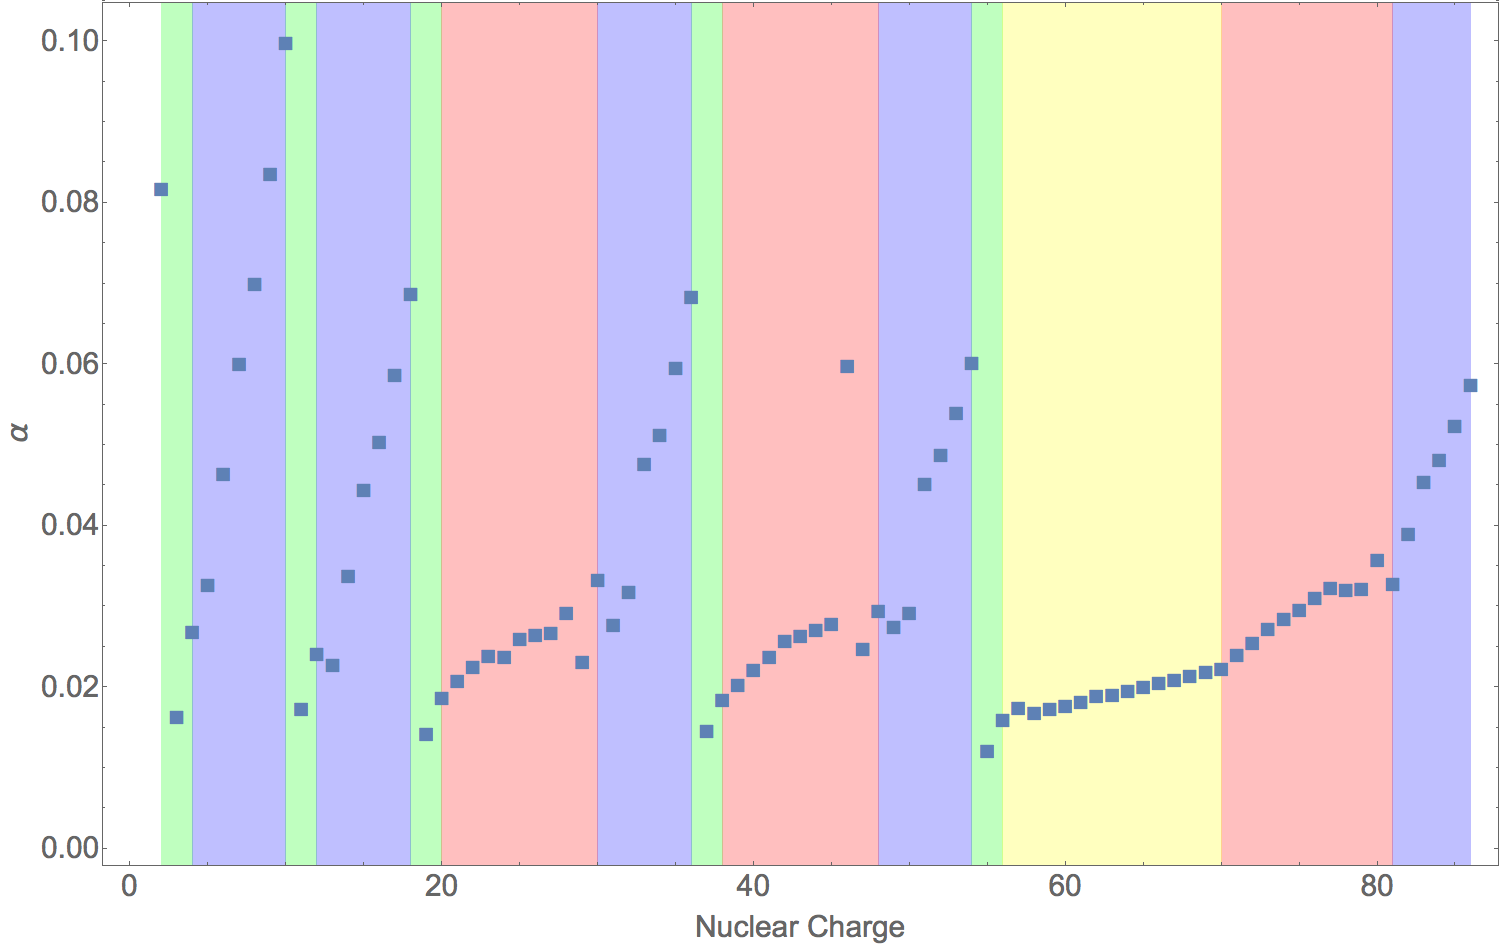
\includegraphics[width=1\textwidth]{Figures/BS_non_rel_alpha.png}
\caption[Scatter plot of the $\alpha$ parameter vs. nuclear charge.]
{Scatter plot of the $\alpha$ parameter vs. nuclear charge. Regions of the plot are shaded based on periodic table block regions. The s block is green, the p block is blue, the d block is red and the f block is yellow. There is a distinct pattern where the value of $\alpha$ increases along a row until a noble gas is reached. Also note how the rate of the increase changes at periodic table block boundaries.}
\label{fig:BS_non_rel_alpha}
\end{figure}

\begin{figure}
\center
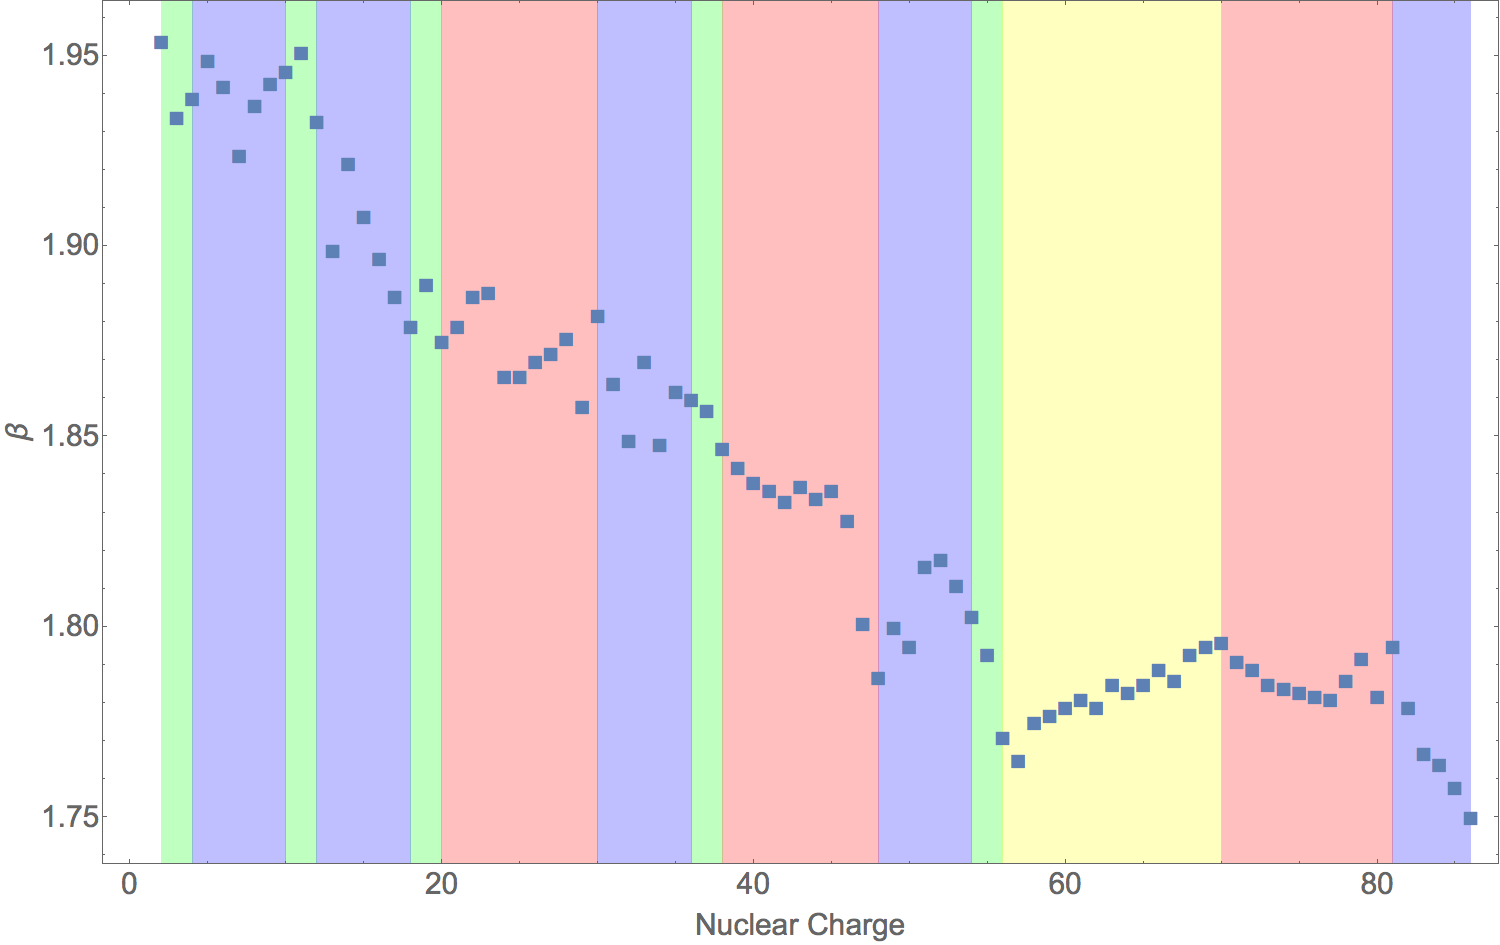
\includegraphics[width=1\textwidth]{Figures/BS_non_rel_beta.png}
\caption[Scatter plot of the $\beta$ parameter vs. nuclear charge.]
{Scatter plot of the $\beta$ parameter vs. nuclear charge. Regions of the plot are shaded based on periodic table block regions. The s block is green, the p block is blue, the d block is red and the f block is yellow. There is a general trend of the value of $\beta$ to decrease as the nuclear charge grows larger.}
\label{fig:BS_non_rel_beta}
\end{figure}

\begin{figure}
\centering
\begin{subfigure}[b]{0.49\textwidth}
	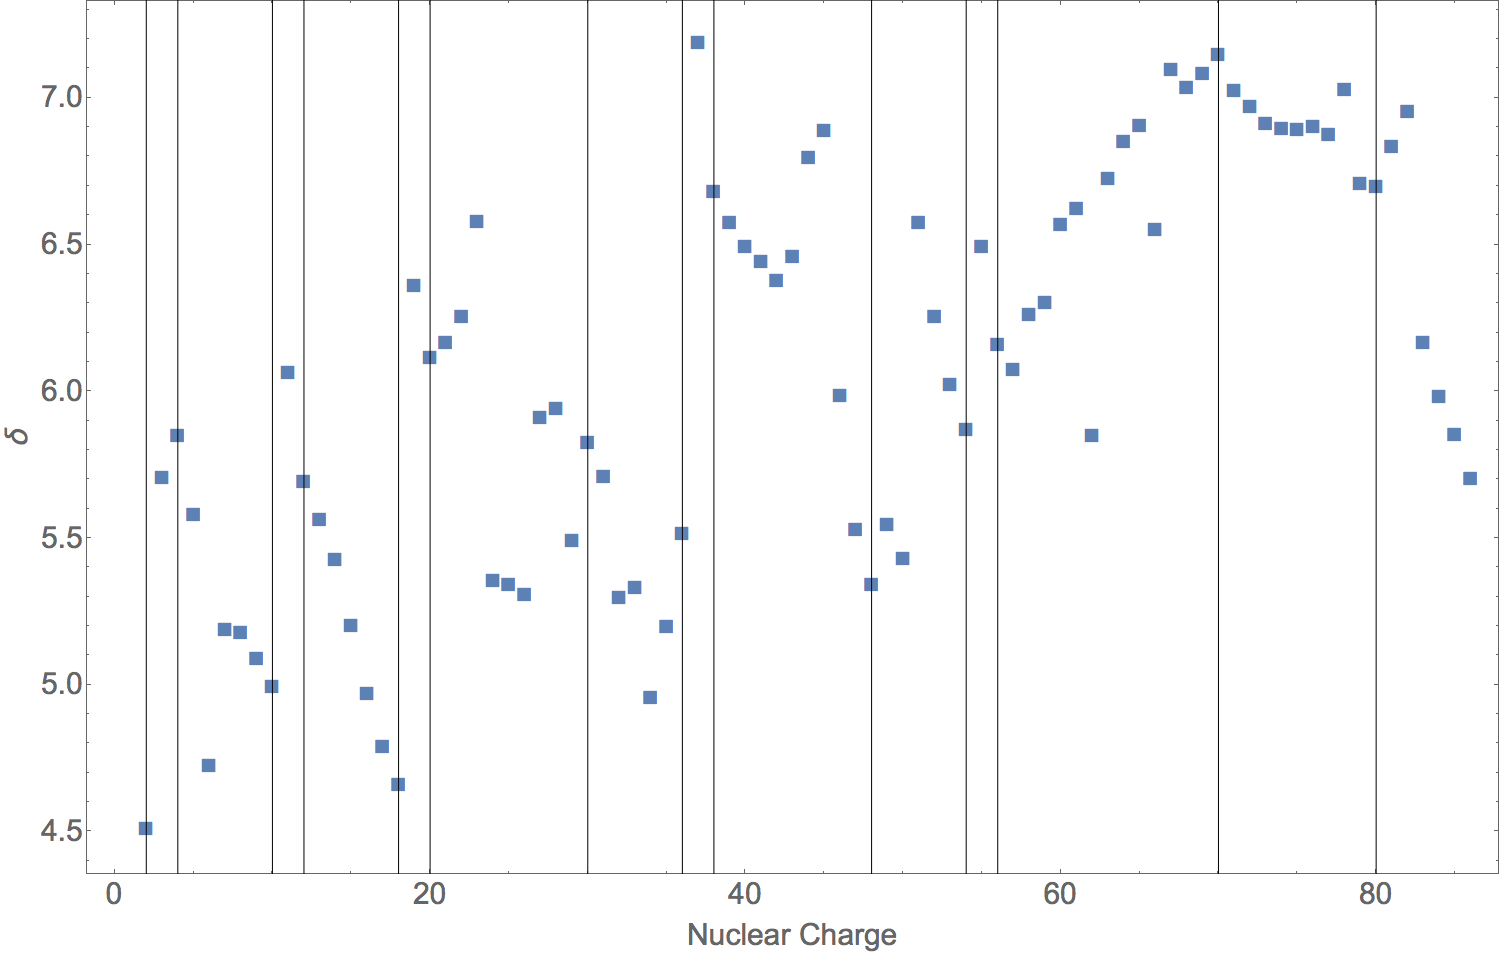
\includegraphics[width=\textwidth]{Figures/BS_non_rel_delta.png}
	\caption{$\delta$}
\end{subfigure}
\begin{subfigure}[b]{0.49\textwidth}
	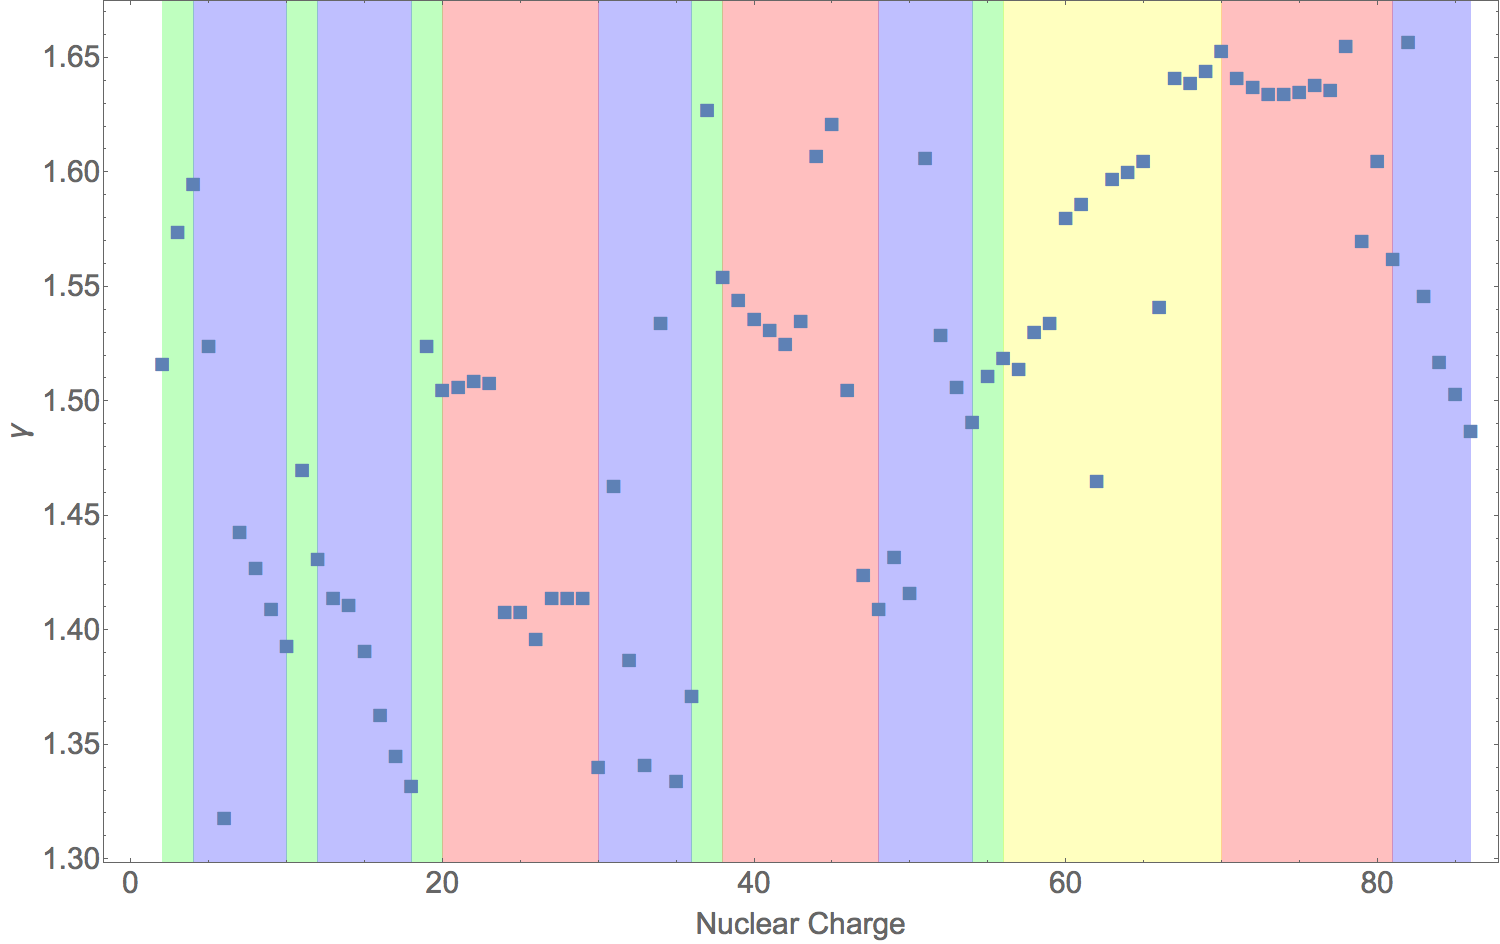
\includegraphics[width=\textwidth]{Figures/BS_non_rel_gamma.png}
	\caption{$\gamma$}
\end{subfigure}	
\caption[Scatter plots of the $\delta$ and $\gamma$ parameters.]{Scatter plots of the $\delta$ and $\gamma$ parameters. Regions of the plot are shaded based on periodic table block regions. The s block is green, the p block is blue, the d block is red and the f block is yellow. There are no clear trends with respect to the nuclear charge.}
\label{fig:BS_non_rel_delt_gamm}
\end{figure}

As for the relativistic basis sets, we can see from Figure \ref{fig:BS_rel_alpha} that the trend in $\alpha$ from the non-relativistic basis sets mostly holds, however there is a slight change in the trend starting at thallium. There is a substantial drop in the value of $\alpha$ when changing from the d to the p block in the relativistic basis sets which is not seen in the non-relativistic sets. We can also see that the change in $\alpha$ for the relativistic basis sets is much larger going through the d block than the change for the non-relativistic basis sets. As for the other WTBS parameters, the trends in the relativistic basis sets are mostly consistent with their non-relativistic counterparts. Figures for the remaining parameters are given in Figures \ref{fig:BS_rel_beta} and \ref{fig:BS_rel_delt_gamm}.

\begin{figure}
\center
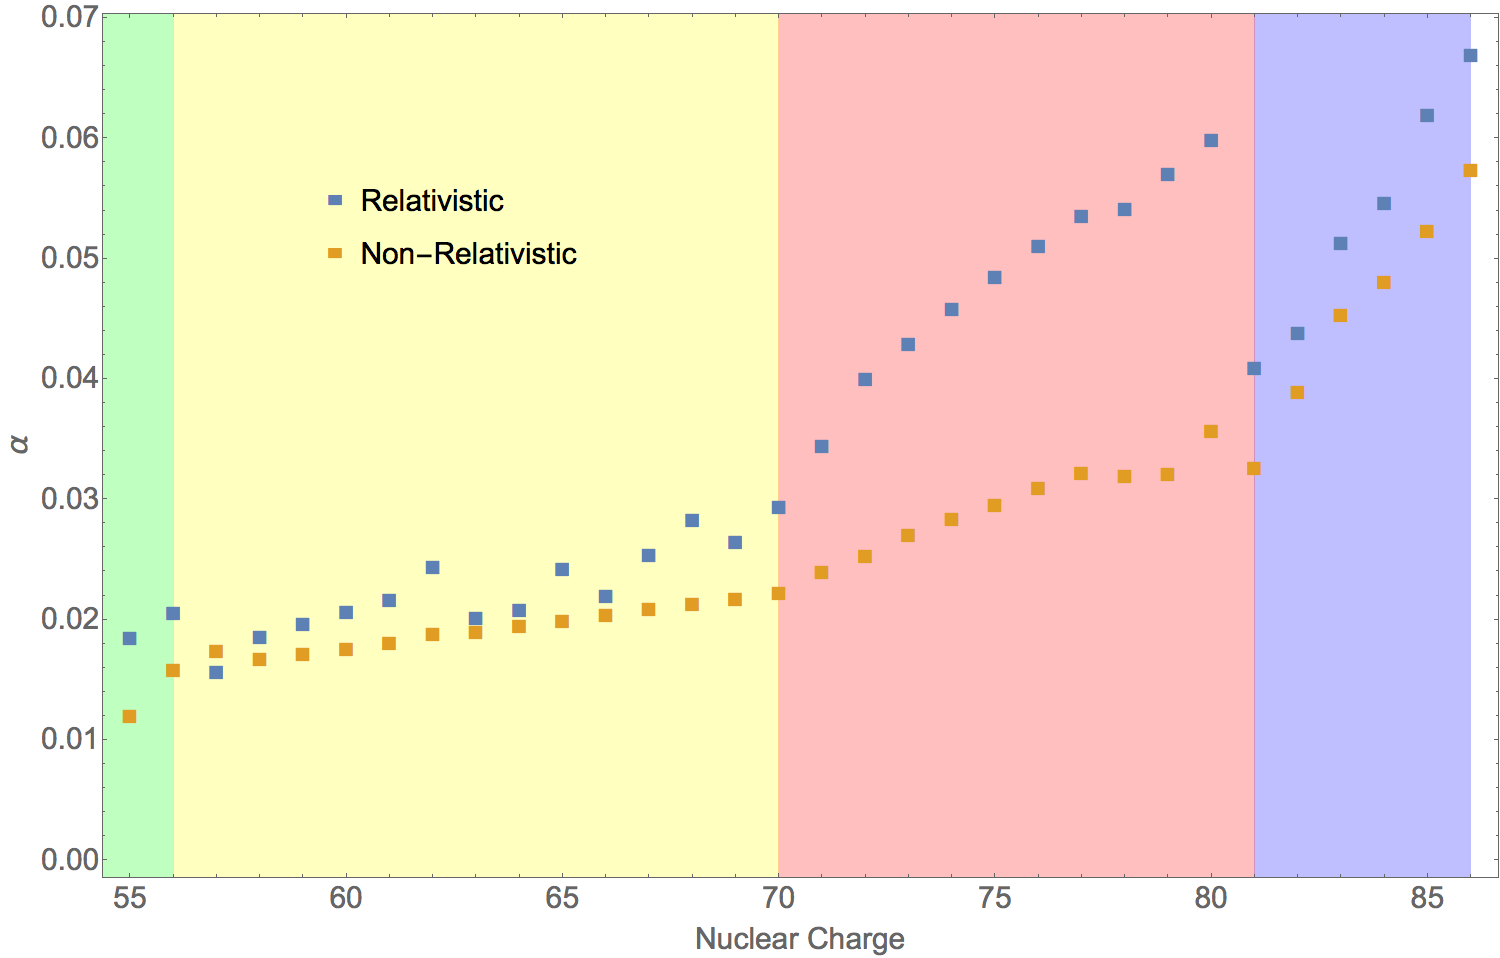
\includegraphics[width=1\textwidth]{Figures/BS_rel_alpha.png}
\caption[Scatter plot of the relativistic and non-relativistic $\alpha$ parameters vs. nuclear charge.]
{Scatter plot of the relativistic and non-relativistic $\alpha$ parameters vs. nuclear charge. Regions of the plot are shaded based on periodic table block regions. The s block is green, the p block is blue, the d block is red and the f block is yellow.}
\label{fig:BS_rel_alpha}
\end{figure}

\begin{figure}
\center
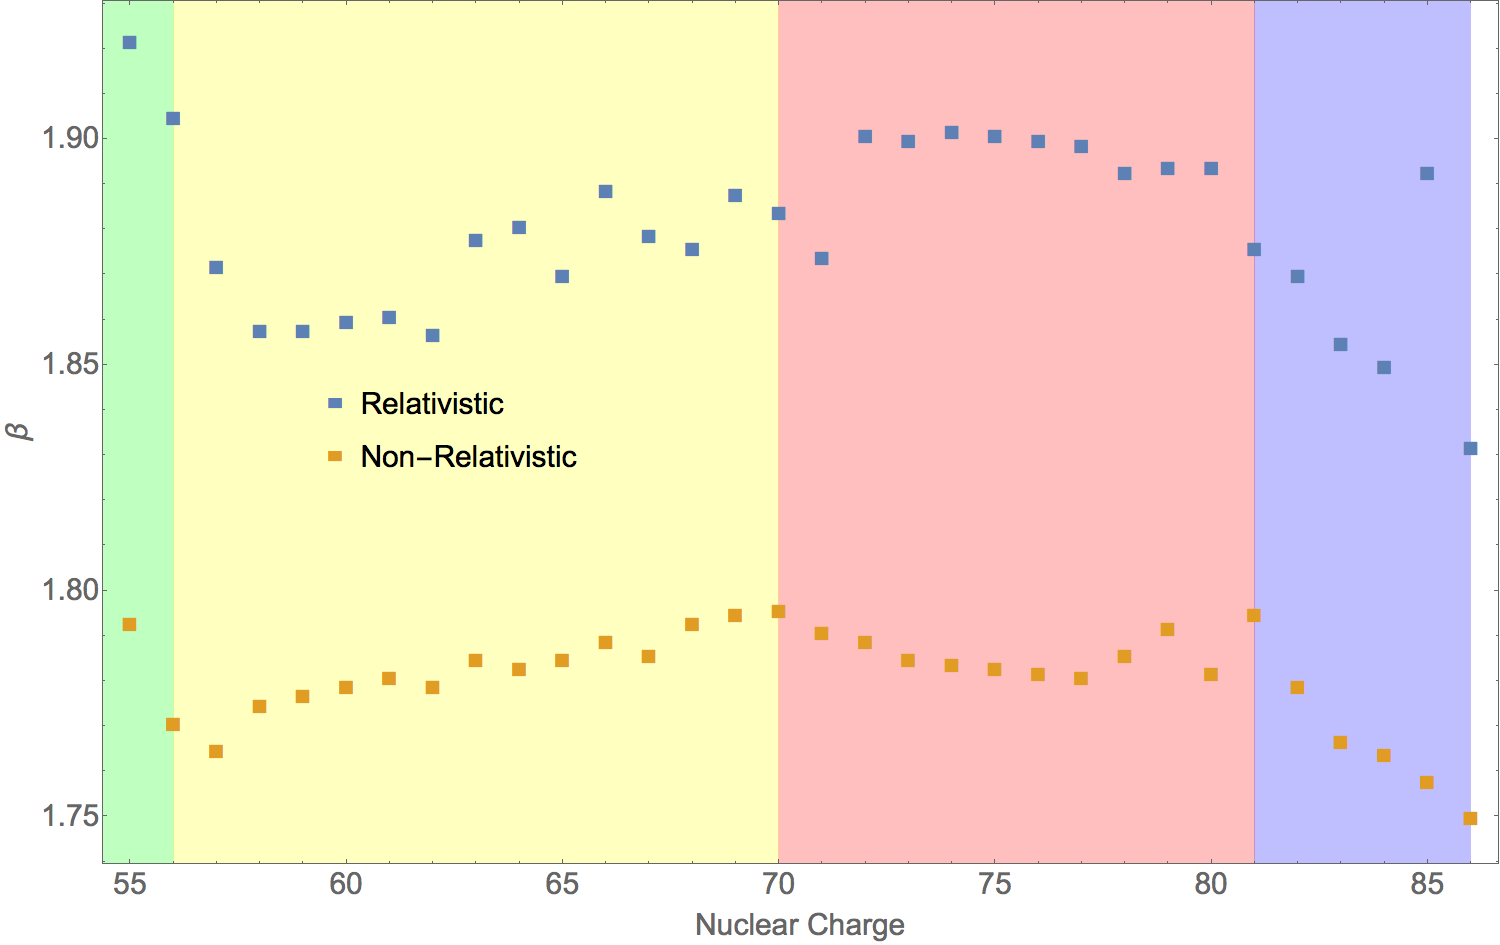
\includegraphics[width=1\textwidth]{Figures/BS_rel_beta.png}
\caption[Scatter plot of the relativistic and non-relativistic $\beta$ parameters vs. nuclear charge.]
{Scatter plot of the relativistic and non-relativistic $\beta$ parameters vs. nuclear charge. Regions of the plot are shaded based on periodic table block regions. The s block is green, the p block is blue, the d block is red and the f block is yellow.}
\label{fig:BS_rel_beta}
\end{figure}

\begin{figure}
\centering
\begin{subfigure}[b]{0.49\textwidth}
	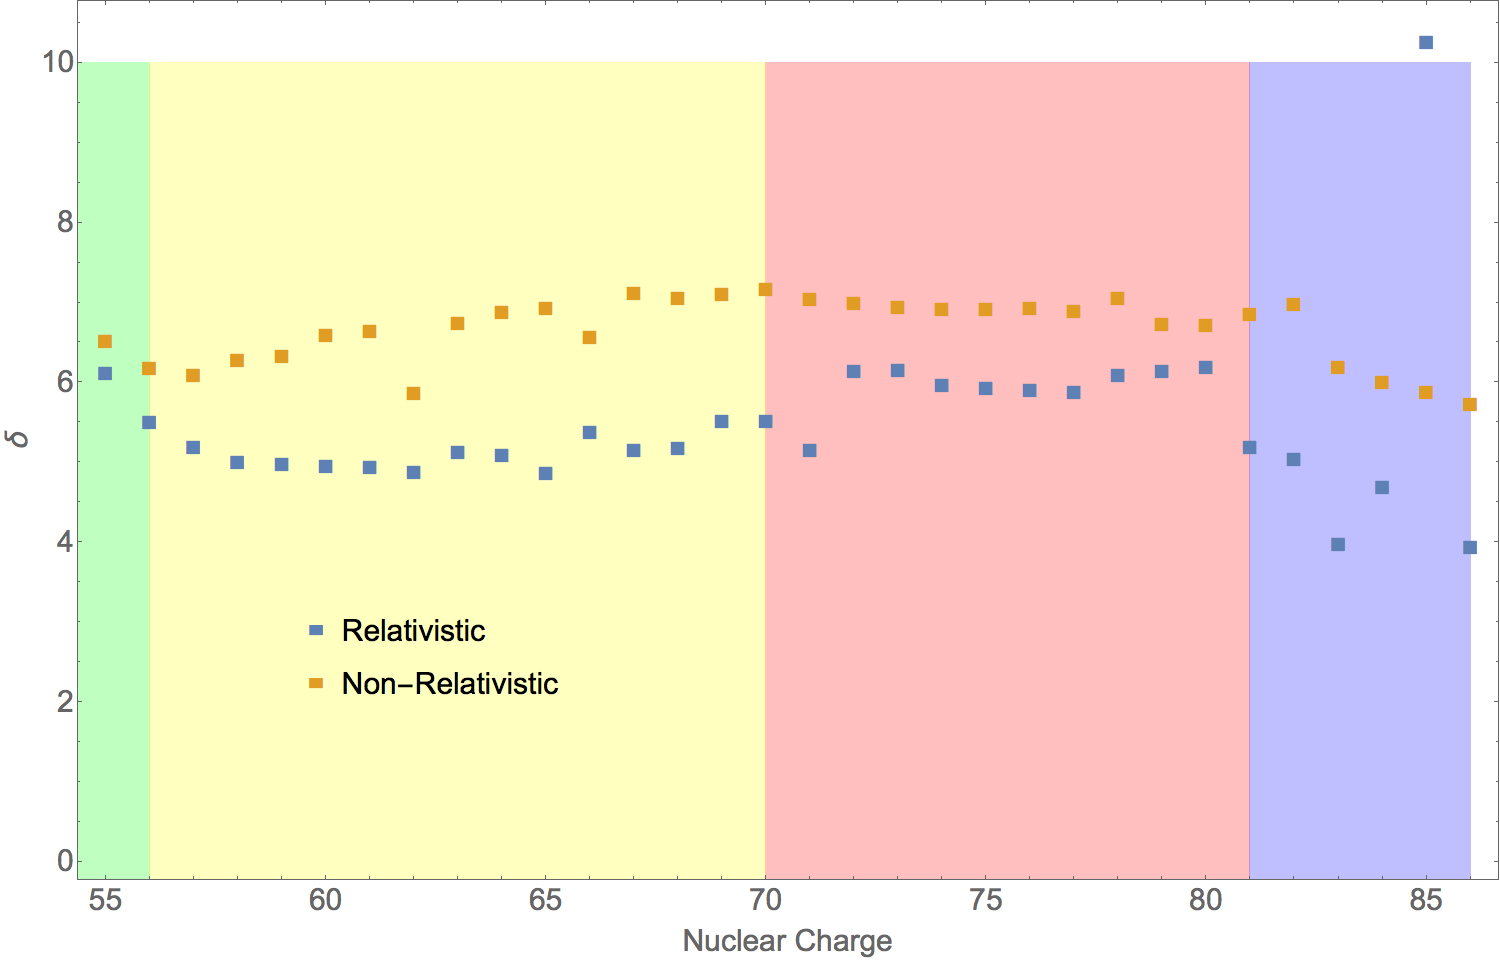
\includegraphics[width=\textwidth]{Figures/BS_rel_delta.png}
	\caption{$\delta$}
\end{subfigure}
\begin{subfigure}[b]{0.49\textwidth}
	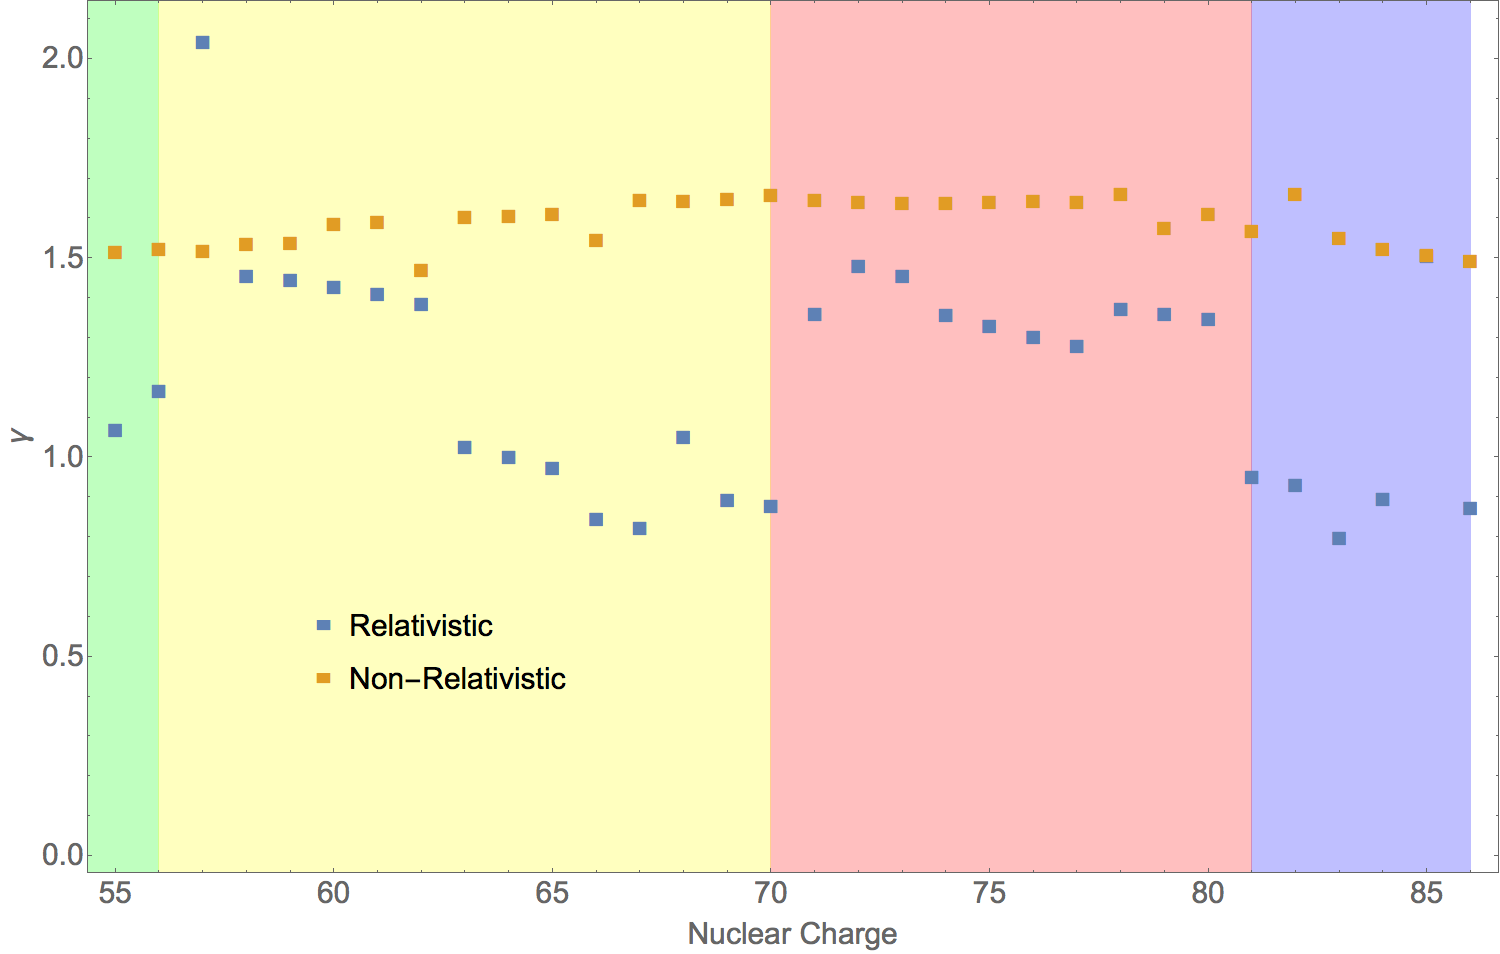
\includegraphics[width=\textwidth]{Figures/BS_rel_gamma.png}
	\caption{$\gamma$}
\end{subfigure}	
\caption[Scatter plot of the relativistic and non-relativistic $\delta$ and $\gamma$ parameters.]{Scatter plot of the relativistic and non-relativistic $\delta$ and $\gamma$ parameters. Regions of the plot are shaded based on periodic table block regions. The s block is green, the p block is blue, the d block is red and the f block is yellow.}
\label{fig:BS_rel_delt_gamm}
\end{figure}


\chapter{Conclusions and Future Work}

In this thesis I have illustrated how even small problems in computational quantum chemistry can benefit from parallel computation. I have done this both in the internal sense, where I rewrote the DFRATOM program to calculate the electronic structure of atoms on GPUs, and in the external sense, where I designed an algorithm that very effectively optimizes basis sets. This chapter will be broken up into two sections: the first which covers the rewriting of DFRATOM into cudaDFRATOM, and the second one which summarizes the results of basis set optimization using cudaDFRATOM and rwtbs.

\section{cudaDFRATOM}
By harnessing the power of GPUs, I was able get the cudaDFRATOM program to accelerate the biggest bottleneck of these calculations, the evaluation of the two-electron integrals, by almost a factor of 20. This changes the bottleneck to be the matrix operations required in SCF. As a result, the total speedup is only about 2-4 times faster than the original DFRATOM program. While this is not as much of an increase as we originally hoped, it is still a very big improvement on the original program.

It is also worth pointing out that as the problems get larger, the speedup gets larger as well. This indicates that the algorithms written for this program could potentially work even better on even larger problems such as molecules. Modifications required to make the algorithms work on molecules are as follows. 

One could implement direct SCF. As the amount of two-electron integrals grows, it becomes impractical to try and store them all in memory. Instead, in the direct SCF algorithm, the integrals are calculated and consumed as needed. The current program has the following flow: the threads are mapped to all the integrals, all the integrals are calculated and stored in memory, and then all the integrals are used to form the \textbf{P} and \textbf{Q} matrices. If we wish to reuse as much of the code I've written as possible, the direct SCF implementation would work as follows. First we would map the threads to a chunk of the integrals, then we could calculate only that chunk, and then we would build up only the elements of the \textbf{P} and \textbf{Q} that use those integrals. Now, we no longer need these integrals, so we can throw them away and start the calculation of a new chunk. We would then loop over these steps until the the \textbf{P} and \textbf{Q} matrices have been completely calculated. The mapping takes very little time to calculate, so the fact that we are calling it so many times would have relatively little impact on performance. 

One could also add some prescreening of the integrals to determine a rough estimate of their order of magnitude. If a particular integral is very close to zero, the effect it has on the calculation is relatively negligible. Therefore we could skip the calculation of this integral, and there would be almost no impact on the accuracy of the calculation. Due to how GPUs perform the calculations in warps, we would need to presort the integrals so that the ones that are likely to be close to zero are grouped together in order to maximize the returns of this procedure.

One would also need to alter the mapping algorithm so that it can handle calculations of different point groups. Atoms have spherical symmetry, meaning we can eliminate the need to calculate a lot of the integrals because many of them will be symmetrically the same. But this would not be the case in systems that have no symmetry, so we would need to change the mapping accordingly. This would actually be very simple to change, as we would just need to write nearly identical code for each symmetry that we would want to support.

One final comment regarding cudaDFRATOM is the algorithm to form the \textbf{P} and \textbf{Q} matrices. I am still not completely satisfied with the current state of this part of the code. It is quite complicated and inelegant. It would seem to me that there should be a better way of performing this calculation, but so far I have been unable to improve upon the version that appears in this thesis. One possible approach would be to break up the calculation of the matrices into two different subroutines: one that calculates \textbf{P} and one that calculates \textbf{Q}. The calculation of \textbf{P} can be reformed into a simple matrix multiplication problem, but \textbf{Q} requires many conditional statements as a result of having to deal with the math of open shells. I did not try this as I believed the main bottleneck was reading the two-electron integrals. Therefore, I only wanted to have to read them once to reduce the amount of global memory reads as possible. But it might be the case that specialized code for each matrix could outperform generalized code for both.

\section{Basis Set Optimization}
This thesis also covered the optimization of new basis sets. I used a novel algorithm that almost entirely eliminates the need for human involvement in the optimization process. It produces useful accurate basis sets, that are practically guarantied to be as small as possible. I have optimized non-relativistic basis sets for the elements helium through radon. I have also optimized relativistic basis sets for the elements caesium through radon. Future work in the area would be the optimization of relativistic basis sets for the rest of the periodic table. Care must be taken when optimizing sets for the seventh row elements, because the assumption made for kinetic balancing begins to break down there. As a result, early attempts to optimize basis sets for these elements have proven to be prone to prolapsing. As a result, the method of automating the optimization process should be used with caution in this range, as the results it produces may erroneously appear to be successful. 

Further work that could be done includes modifications to the cudaDFRATOM program to support basis sets other than WTBS, and also to include other optimization algorithms than \textit{\textbf{newuoa}}, which might be less prone to generating prolapsing basis sets. cudaDFRATOM also includes the option to optimize a different set of $\zeta$s for different groups of spinor symmetries. Therefore, it might be best to try and optimize basis sets that have grouped the s and p type spinors into one group and the d and f type spinors in another. The logic of this is that relativity has different effects on these two groups, so it might be best to try and separate the two so that each gets its own set of specialized basis functions.

%TCIMACRO{
%\TeXButton{liography in contents}{\clearpage\addcontentsline{toc}{chapter}{Bibliography}
%\singlespacing
%}}%
%BeginExpansion
\clearpage\addcontentsline{toc}{chapter}{Bibliography}
\singlespacing
%
%EndExpansion
%
%
%
%
%
%
%
%
%
%
%
%
%
%
%
%
%
%
%
%
%
%
%
%
%
%
%
%
%
%
%
%
%
%
%
%
%
%
%dont forget this if you want the bibliography to show up on the contents page
\bibliographystyle{initunsrt}
\bibliography{thesis}
\bigskip 
%Generates the bibliography. You have to specify the source bib files and the biblio style 

%TCIMACRO{
%\TeXButton{Appendices}{\appendix
%}}%
%BeginExpansion
\appendix
\chapter{cudaDFRATOM Input and Output files}
\label{app:cudaDFRATOM_inp}

This appendix shows cudaDFRATOM input files for a few common calculations. The output files are also given.

\section{Single Point Energy with predefined WTBS parameters}
This input file will perform a calculation on lead using predefined well-tempered basis set (WTBS) parameters. It uses the ``autogen" option to automatically generate electron configurations.

\lstinputlisting[caption={Input file for calculating the single point energy of Pb.}, language={}, basicstyle=\ttfamily\tiny\color{black}]{appendix/inp_out_files/82Pb_gauss_35s30p-30p+25d-25d+20f-20f+.inp}
\lstinputlisting[caption={Output file for calculating the single point energy of Pb.}, language={}, basicstyle=\ttfamily\tiny\color{black}]{appendix/inp_out_files/82Pb_gauss_35s30p-30p+25d-25d+20f-20f+.log}

\section{Optimizing a Basis Set for a Specific Electron Configuration}
\label{sec:opt_bs_spec}
This input file will optimize a WTBS basis set for protactinium with a specific electron configuration. Note that in the output file, the ``freeel" variable is set to 1. ``freeel" only matters if ``autogen" is set to true, the actual number of electrons in open shells is determined from the electron configurations that are read in.

\lstinputlisting[caption={Input file for Pa basis set optimization calculation.}, language={}, basicstyle=\ttfamily\tiny\color{black}]{appendix/inp_out_files/91Pa_35s30p-30p+25d-25d+20f-20f+.inp}
\lstinputlisting[caption={Output file for Pa basis set optimization calculation.}, language={}, basicstyle=\ttfamily\tiny\color{black}]{appendix/inp_out_files/91Pa_35s30p-30p+25d-25d+20f-20f+.log}

\section{Single Point Energy using a predefined Basis Set}
This input file will perform a single point energy calculation on protactinium using the basis optimized in Section \ref{sec:opt_bs_spec}.

\lstinputlisting[caption={Input file for calculating the single point energy of Pa using a predefined basis set.}, language={}, basicstyle=\ttfamily\tiny\color{black}]{appendix/inp_out_files/91Pa_35s30p-30p+25d-25d+20f-20f+_readin.inp}
\lstinputlisting[caption={Output file for calculating the single point energy of Pa using a predefined basis set.}, language={}, basicstyle=\ttfamily\tiny\color{black}]{appendix/inp_out_files/91Pa_35s30p-30p+25d-25d+20f-20f+_readin.log}
\chapter{Scripts for cudaDFRATOM}
These are the scripts for automating the optimization of basis sets using cudaDFRATOM.

\lstinputlisting[caption={BS\_sub\_auto.sh: Generate and submit input files.}, language={}, basicstyle=\ttfamily\tiny\color{black}]{appendix/auto_scripts/BS_sub_auto.sh}
\lstinputlisting[caption={BS\_get\_best.sh: Find the best basis set.}, language={}, basicstyle=\ttfamily\tiny\color{black}]{appendix/auto_scripts/BS_get_best.sh}

%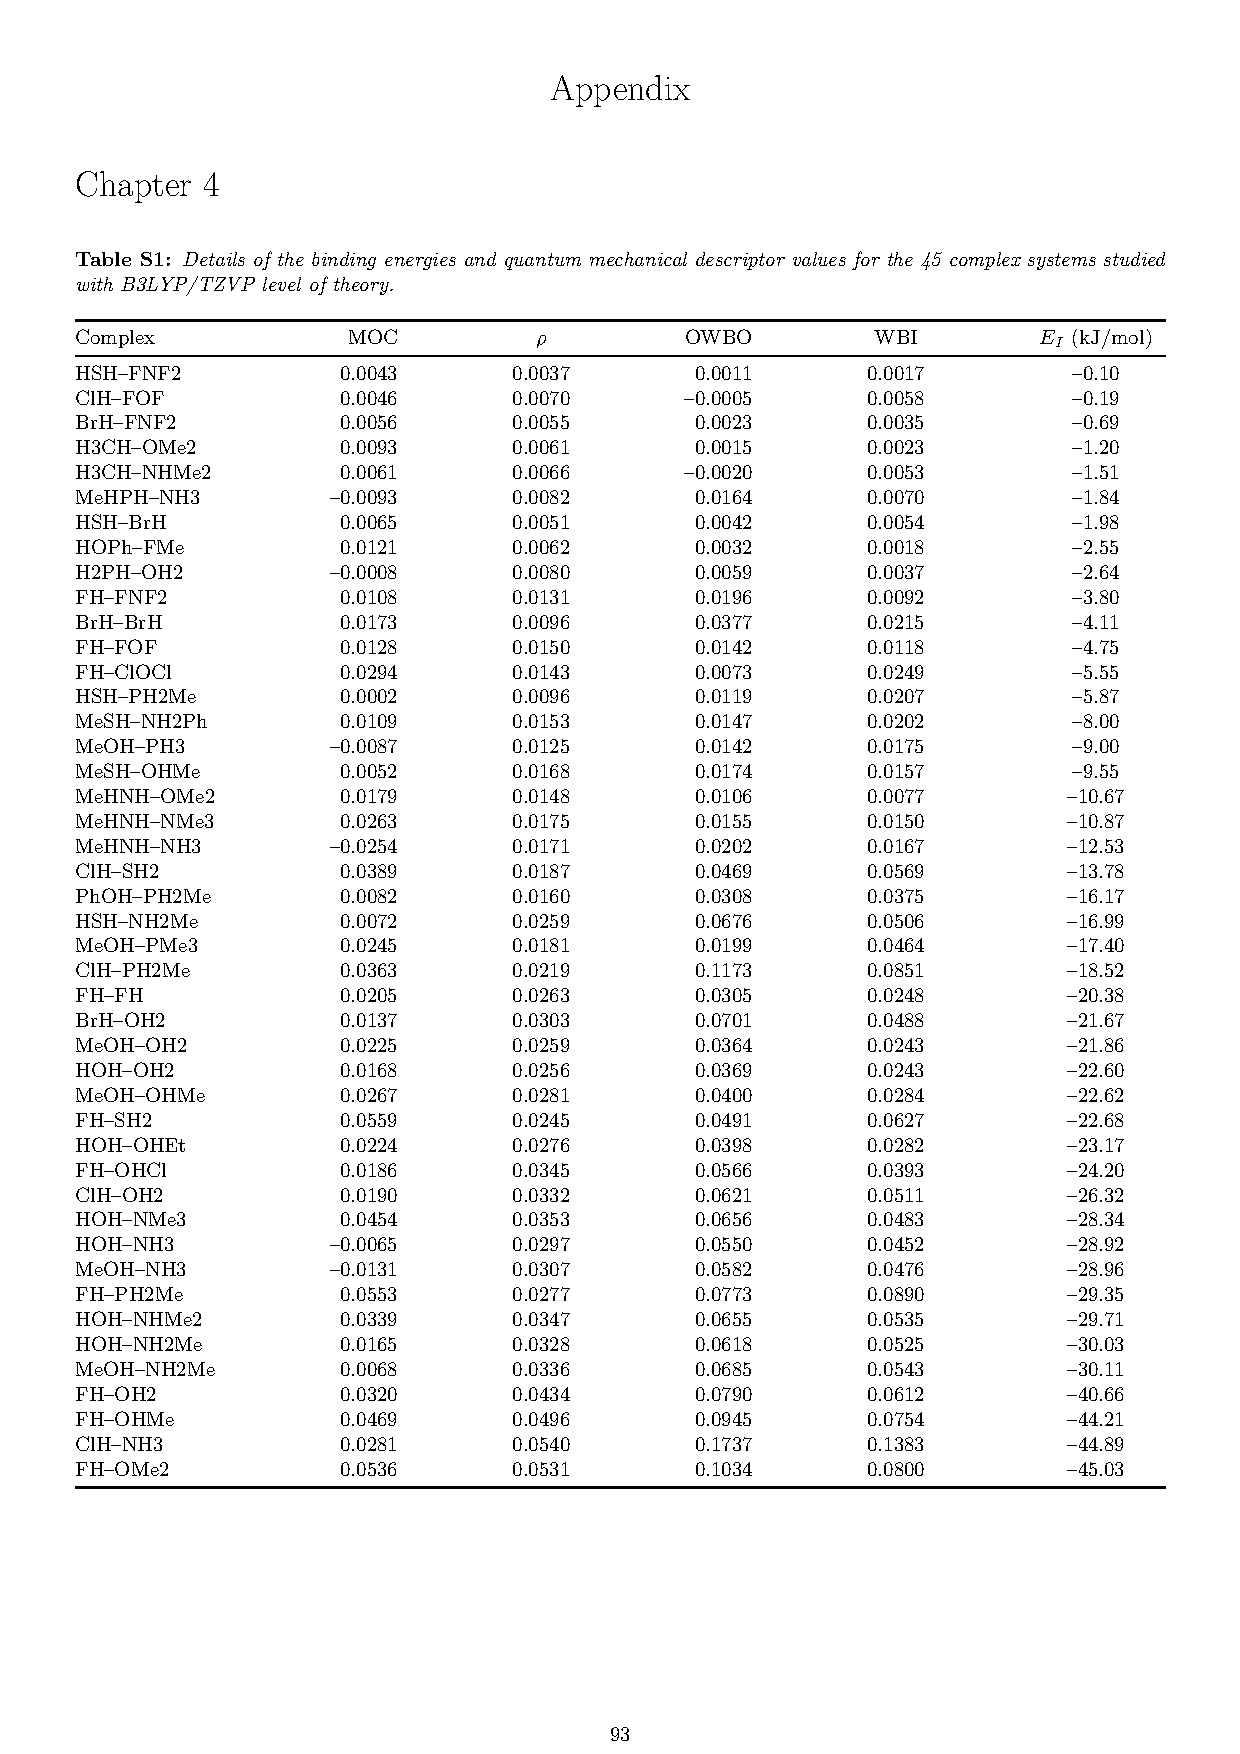
\includepdf[pages=1-10]{supp.pdf}
%
%EndExpansion
%
%
%
%
%
%
%
%
%
%
%
%
%
%
%
%
%
%
%
%
%
%
%
%
%
%
%
%
%
%
%
%
%
%
%
%
%
%
%The chapters after this tab are all appendices

\end{document}
